% ==============================================================================
% PHẦN BÁO CÁO CHỦ ĐỀ 1: DATA STORAGE & MANAGEMENT (MS SQL SERVER VS. NEO4J)
% Thành viên phụ trách: Trần Quốc Hiền - 2310992 (Chủ đề 1)
%
% HƯỚNG DẪN TÍCH HỢP VÀO FILE main.tex TRÊN OVERLEAF:
%   1. Tải file này vào thư mục report/section_4_1_data_storage.tex
%      và 3 ảnh vào thư mục report/images/:
%        - report/images/topic1_neo4j_store_breakdown.png
%        - report/images/topic1_storage_comparison.png
%        - report/images/topic1_evolution_query.png
%   2. Tại mục \subsection{Data storage \& management} trong main.tex:
%      Thay dòng (TEXT GOES HERE.) bằng:
%        % ==============================================================================
% PHẦN BÁO CÁO CHỦ ĐỀ 1: DATA STORAGE & MANAGEMENT (MS SQL SERVER VS. NEO4J)
% Thành viên phụ trách: Trần Quốc Hiền - 2310992 (Chủ đề 1)
%
% HƯỚNG DẪN TÍCH HỢP VÀO FILE main.tex TRÊN OVERLEAF:
%   1. Tải file này vào thư mục report/section_4_1_data_storage.tex
%      và 3 ảnh vào thư mục report/images/:
%        - report/images/topic1_neo4j_store_breakdown.png
%        - report/images/topic1_storage_comparison.png
%        - report/images/topic1_evolution_query.png
%   2. Tại mục \subsection{Data storage \& management} trong main.tex:
%      Thay dòng (TEXT GOES HERE.) bằng:
%        % ==============================================================================
% PHẦN BÁO CÁO CHỦ ĐỀ 1: DATA STORAGE & MANAGEMENT (MS SQL SERVER VS. NEO4J)
% Thành viên phụ trách: Trần Quốc Hiền - 2310992 (Chủ đề 1)
%
% HƯỚNG DẪN TÍCH HỢP VÀO FILE main.tex TRÊN OVERLEAF:
%   1. Tải file này vào thư mục report/section_4_1_data_storage.tex
%      và 3 ảnh vào thư mục report/images/:
%        - report/images/topic1_neo4j_store_breakdown.png
%        - report/images/topic1_storage_comparison.png
%        - report/images/topic1_evolution_query.png
%   2. Tại mục \subsection{Data storage \& management} trong main.tex:
%      Thay dòng (TEXT GOES HERE.) bằng:
%        % ==============================================================================
% PHẦN BÁO CÁO CHỦ ĐỀ 1: DATA STORAGE & MANAGEMENT (MS SQL SERVER VS. NEO4J)
% Thành viên phụ trách: Trần Quốc Hiền - 2310992 (Chủ đề 1)
%
% HƯỚNG DẪN TÍCH HỢP VÀO FILE main.tex TRÊN OVERLEAF:
%   1. Tải file này vào thư mục report/section_4_1_data_storage.tex
%      và 3 ảnh vào thư mục report/images/:
%        - report/images/topic1_neo4j_store_breakdown.png
%        - report/images/topic1_storage_comparison.png
%        - report/images/topic1_evolution_query.png
%   2. Tại mục \subsection{Data storage \& management} trong main.tex:
%      Thay dòng (TEXT GOES HERE.) bằng:
%        \input{report/section_4_1_data_storage}
%      (hoặc copy-paste toàn bộ nội dung từ \subsubsection{...} đến trước phần
%      comment ở cuối file này).
%   3. Cập nhật Bảng 1 (Danh sách thành viên) và nối các \bibitem{t1_...} ở cuối
%      file này vào khối \begin{thebibliography} của main.tex.
% ==============================================================================

\subsubsection{Khái niệm chung về Data Storage và Data Management}

\textbf{Data Storage (Lưu trữ dữ liệu)} là quá trình tổ chức, cấu trúc hóa và duy trì dữ liệu dưới các định dạng nhị phân phù hợp trên thiết bị lưu trữ thứ cấp (SSD/HDD) nhằm bảo đảm độ bền lâu dài, hiệu quả truy xuất và khả năng mở rộng khi khối lượng dữ liệu gia tăng. Thành phần đảm nhiệm trực tiếp chức năng này bên trong một hệ quản trị cơ sở dữ liệu (DBMS) là \textbf{Storage Engine} -- lớp phần mềm cốt lõi chịu trách nhiệm cấp phát không gian đĩa, quản lý bộ nhớ đệm (\textit{Buffer Pool} hoặc \textit{Page Cache}) và duy trì nhật ký giao dịch (\textit{Transaction Log}) phục vụ khôi phục dữ liệu~\cite{t1_date2004,t1_silberschatz2019}.

\textbf{Data Management (Quản trị dữ liệu)} bao gồm tập hợp các cơ chế vận hành trên dữ liệu đã lưu trữ: kiểm soát toàn vẹn ngữ nghĩa và ràng buộc tham chiếu, thực thi truy vấn, xử lý giao dịch (\textit{Transaction}), điều khiển đồng thời, thu hồi không gian trống và bảo đảm tính bền vững sau sự cố. Kiến trúc lưu trữ ở tầng vật lý ảnh hưởng trực tiếp đến chi phí I/O, hiện tượng phân mảnh trang đĩa, dung lượng lưu trữ tiêu thụ cũng như mức độ linh hoạt khi nghiệp vụ thay đổi.

Trong bài toán thực tế của nhóm là nền tảng sàn thương mại điện tử đa gian hàng (\textit{Multi-Vendor E-Commerce Platform}, CSDL \texttt{ECommerceDB}), hệ thống vừa đòi hỏi tính nhất quán chặt chẽ ở các bảng giao dịch cốt lõi (\texttt{Users}, \texttt{Sellers}, \texttt{Orders}, \texttt{Order\_Details}, \texttt{Vouchers}), vừa phát sinh bài toán đặc trưng về \textbf{thuộc tính biến thể sản phẩm linh hoạt}: sản phẩm thuộc ngành hàng \textit{Smartphones} cần lưu \texttt{storage\_gb}, \texttt{ram\_gb}, \texttt{screen\_inch}, \texttt{chipset}; ngành hàng \textit{Laptops} cần \texttt{cpu\_model}, \texttt{gpu\_model}, \texttt{os\_name}; ngành hàng \textit{Fashion} cần \texttt{apparel\_size}, \texttt{material}, \texttt{fit\_style}; còn ngành hàng \textit{Books} lại cần \texttt{author\_name}, \texttt{publisher}, \texttt{page\_count} và \texttt{isbn\_note}. Cách tiếp cận bài toán này phản ánh rõ sự đối lập giữa hai triết lý thiết kế dữ liệu:

\begin{itemize}
  \item \textbf{MS SQL Server (Schema-on-Write):} Yêu cầu khai báo tường minh toàn bộ cấu trúc bảng, kiểu dữ liệu và các ràng buộc (\texttt{PRIMARY KEY}, \texttt{FOREIGN KEY}, \texttt{CHECK}, \texttt{NOT NULL}, \texttt{UNIQUE}) trước khi ghi dữ liệu. Mọi thao tác \texttt{INSERT} hoặc \texttt{UPDATE} đều được kiểm tra nghiêm ngặt ngay tại thời điểm ghi nhằm bảo đảm tính nhất quán cao.
  \item \textbf{Neo4j (Schema-Optional):} Lưu trữ theo mô hình đồ thị thuộc tính có nhãn (\textit{Labeled Property Graph}), cho phép các nút cùng nhãn mang tập thuộc tính khác nhau và bổ sung thuộc tính mới ngay trong quá trình ghi mà không cần chỉnh sửa lược đồ tĩnh, đồng thời vẫn hỗ trợ \textit{Indexes} và \textit{Constraints} để kiểm soát các khóa định danh quan trọng~\cite{t1_robinson2015,t1_neo4jops}.
\end{itemize}

\subsubsection{Đặc trưng cơ chế Data Storage và Data Management trong MS SQL Server}

\paragraph{Mô hình tổ chức và thiết kế dữ liệu cho thuộc tính động:}
MS SQL Server tổ chức dữ liệu logic dưới dạng bảng hai chiều (\textit{Tables, Rows, Columns}) và cung cấp hai cấu trúc lưu trữ vật lý nền tảng cho dữ liệu hàng (\textit{Rowstore})~\cite{t1_delaney2012,t1_mspages}:
\begin{itemize}
  \item \textbf{Heap:} Bảng không có \textit{Clustered Index}; các dòng dữ liệu được lưu tự do không theo thứ tự khóa và được định vị thông qua địa chỉ vật lý \textbf{RID} (\textit{FileID:PageID:SlotID}).
  \item \textbf{Clustered Index:} Tổ chức bảng dưới dạng cây cân bằng \textbf{B+Tree}, trong đó các nút lá chứa trực tiếp toàn bộ dữ liệu dòng được sắp xếp theo thứ tự khóa cụm (mặc định gắn với \texttt{PRIMARY KEY}).
\end{itemize}

Khi mô hình hóa tập thuộc tính biến thể đa dạng trên nền tảng chuẩn hóa quan hệ (1NF--3NF), các hệ thống dùng SQL Server thường áp dụng một trong ba hướng thiết kế sau:
\begin{itemize}
  \item \textbf{Mô hình Entity--Attribute--Value (EAV):} Tách danh mục thuộc tính sang bảng \texttt{Attributes} và lưu từng cặp thuộc tính--giá trị dưới dạng các dòng dọc trong bảng \texttt{Variant\_Attr\_Values}. EAV cho phép thêm thuộc tính mới bằng lệnh \texttt{INSERT} (không cần DDL), nhưng làm tăng mạnh số dòng dữ liệu, giảm an toàn kiểu dữ liệu (thường phải lưu chuỗi \texttt{NVARCHAR}) và phát sinh nhiều phép \texttt{JOIN} khi truy xuất nhiều thuộc tính cùng lúc.
  \item \textbf{Wide Table với Sparse Columns:} Khai báo tất cả thuộc tính của mọi ngành hàng thành các cột trên một bảng rộng kèm từ khóa \texttt{SPARSE NULL}~\cite{t1_mssparse}. Mỗi giá trị \texttt{NULL} trên cột Sparse tiêu thụ \textbf{0 byte} lưu trữ, nhưng mỗi giá trị khác \texttt{NULL} phát sinh thêm 2--4 byte chi phí quản lý trong cấu trúc \textit{Sparse Vector} (chỉ đạt hiệu quả nén khi tỷ lệ \texttt{NULL} cao, thường $\ge$ 20--40\% tùy kiểu dữ liệu) và vẫn phụ thuộc vào lệnh DDL \texttt{ALTER TABLE} khi cần thêm cột mới.
  \item \textbf{Mô hình Hybrid JSON (\texttt{NVARCHAR(MAX)} và kiểu \texttt{json} gốc trên SQL Server 2025):} Giữ các cột giao dịch cốt lõi (\texttt{variant\_id}, \texttt{product\_id}, \texttt{sku}, \texttt{price}, \texttt{stock\_qty}) dưới dạng quan hệ chuẩn định kiểu chặt chẽ, còn tập thuộc tính đặc thù theo ngành hàng được đóng gói vào cột bán cấu trúc. Trước đây, dữ liệu JSON được lưu dưới dạng chuỗi UTF-16 trong \texttt{NVARCHAR(MAX)} kèm ràng buộc \texttt{CHECK} \texttt{(ISJSON(col) = 1)} và cập nhật qua \texttt{JSON\_MODIFY()}. Từ phiên bản \textbf{MS SQL Server 2025}, hệ thống bổ sung kiểu dữ liệu \textbf{\texttt{json} gốc (Native \texttt{json} Data Type)} lưu ở định dạng nhị phân đã phân tích cú pháp sẵn (\textit{pre-parsed binary}) cùng phương thức \texttt{.modify()} trực tiếp, giúp tiết kiệm dung lượng đĩa và giảm chi phí phân tích cú pháp~\cite{t1_msnativejson}.
\end{itemize}

\paragraph{Kiến trúc tệp và trang lưu trữ (Page \& Extent):}
Ở tầng vật lý, mỗi CSDL SQL Server sử dụng ba loại tệp chính: \texttt{.mdf} (tệp dữ liệu chính), \texttt{.ndf} (tệp dữ liệu phụ) và \texttt{.ldf} (tệp nhật ký giao dịch)~\cite{t1_mspages}. Không gian bên trong tệp dữ liệu được chia nhỏ thành các đơn vị lưu trữ chuẩn hóa~\cite{t1_delaney2012,t1_mspages}:
\begin{itemize}
  \item \textbf{Page:} Đơn vị I/O cơ bản có kích thước cố định \textbf{8 KB (8.192 bytes)}, gồm ba vùng chính: (1) \textit{Page Header} (96 bytes đầu chứa mã trang \texttt{m\_pageId}, loại trang \texttt{m\_type}, số dòng \texttt{m\_slotCnt}, vùng trống \texttt{m\_freeCnt}, số bản ghi ma \texttt{m\_ghostRecCnt} và LSN gần nhất \texttt{m\_lsn}); (2) \textit{Data Area} (nơi lưu nối tiếp các dòng dữ liệu); và (3) \textit{Slot Array} ở cuối trang lưu offset trỏ về vị trí từng dòng theo thứ tự logic.
  \item \textbf{Extent:} Gồm \textbf{8 Page liên tiếp}, tương đương \textbf{64 KB}, gồm \textit{Uniform Extent} (cấp phát cho một đối tượng duy nhất) và \textit{Mixed Extent} (chia sẻ giữa tối đa 8 đối tượng nhỏ).
\end{itemize}

\paragraph{Lưu trữ dữ liệu lớn (Allocation Units) và cơ chế nén:}
SQL Server quản lý dữ liệu có kích thước thay đổi thông qua ba \textbf{Allocation Units}~\cite{t1_mspages}:
\begin{itemize}
  \item \textbf{\texttt{IN\_ROW\_DATA}:} Lưu các cột cố định và biến thiên trực tiếp trên trang dữ liệu chính với giới hạn dòng chuẩn tối đa \textbf{8.060 bytes}.
  \item \textbf{\texttt{ROW\_OVERFLOW\_DATA}:} Tự động đẩy các cột độ dài biến thiên (như \texttt{VARCHAR}, \texttt{NVARCHAR}) sang trang tràn dòng khi tổng kích thước dòng vượt quá 8.060 bytes, giữ lại con trỏ 24-byte trên trang gốc.
  \item \textbf{\texttt{LOB\_DATA}:} Lưu trữ các kiểu dữ liệu khối lớn như \texttt{VARCHAR(MAX)}, \texttt{NVARCHAR(MAX)}, \texttt{VARBINARY\allowbreak(MAX)} hoặc \texttt{json} vượt ngưỡng lưu nội dòng.
\end{itemize}

Để tối ưu dung lượng đĩa và I/O bộ nhớ đệm, SQL Server hỗ trợ hai cơ chế nén tích hợp (\texttt{DATA\_COMPRESSION})~\cite{t1_mscomp}: \textbf{Row Compression} chuyển kiểu dữ liệu cố định sang biểu diễn độ dài biến thiên theo giá trị thực và loại bỏ byte đệm trống; trong khi \textbf{Page Compression} kết hợp tuần tự \textit{Row Compression}, \textit{Prefix Compression} (trích xuất tiền tố chung của cột) và \textit{Dictionary Compression} (thay thế giá trị lặp lại toàn trang bằng từ điển nội trang).

\paragraph{Quản lý không gian, phân mảnh và Transaction Log:}
SQL Server theo dõi không gian cấp phát qua các trang bitmap chuyên biệt gồm \textbf{GAM/SGAM} (trạng thái cấp phát Extent), \textbf{PFS} (tỷ lệ chỗ trống của từng Page) và \textbf{IAM} (ánh xạ các Extent thuộc một Allocation Unit)~\cite{t1_mspages}. Khi thêm, sửa hoặc xóa dữ liệu liên tục, hệ thống có thể phát sinh \textbf{Page Split} (tách đôi trang lá B+Tree đã đầy khi chèn khóa mới), \textbf{Forwarded Record} (dòng trên bảng Heap phình to phải dời sang trang khác để lại con trỏ chuyển tiếp), và \textbf{Ghost Record} (đánh dấu logic bản ghi bị xóa hoặc hủy bỏ trên trang lá để tiến trình nền \textit{Ghost Cleanup} thu hồi sau). Quản trị viên bảo trì cấu trúc bằng \texttt{REORGANIZE}/\texttt{REBUILD} và thu hồi dung lượng tệp đĩa bằng \texttt{DBCC SHRINKFILE}. Toàn bộ biến động trên \textit{Buffer Pool} tuân thủ nguyên tắc \textbf{Write-Ahead Logging (WAL)}, kết hợp tiến trình \textbf{Checkpoint} và cơ chế \textbf{REDO/UNDO} từ Transaction Log để đảm bảo phục hồi bền vững~\cite{t1_delaney2012}.

\subsubsection{Đặc trưng cơ chế Data Storage và Data Management trong Neo4j}

\paragraph{Mô hình Labeled Property Graph:}
Neo4j lưu trữ dữ liệu trực tiếp theo mô hình \textbf{Labeled Property Graph (LPG)} gồm ba thành phần cốt lõi~\cite{t1_robinson2015,t1_neo4jops}:
\begin{itemize}
  \item \textbf{Nodes (Nút):} Đại diện cho thực thể (ví dụ \texttt{:User}, \texttt{:Product}, \texttt{:T1VariantProp}); mỗi nút có thể mang một hoặc nhiều nhãn (\textit{Labels}).
  \item \textbf{Relationships (Quan hệ):} Biểu diễn liên kết có hướng và có kiểu giữa nút nguồn và nút đích, ví dụ \texttt{(User)-[:PLACED]->(Order)} hay \texttt{(Product)-\allowbreak[:HAS\_VARIANT]->\allowbreak(Variant)}; mỗi cạnh cũng có thể mang thuộc tính riêng.
  \item \textbf{Properties (Thuộc tính):} Các cặp \textit{Key--Value} linh hoạt gắn trực tiếp lên Node hoặc Relationship.
\end{itemize}

\paragraph{Native Graph Storage và Index-Free Adjacency:}
Neo4j tổ chức dữ liệu đồ thị gốc thành các tệp store vật lý chuyên biệt có kích thước bản ghi cố định trong thư mục dữ liệu~\cite{t1_neo4jops}:
\begin{itemize}
  \item \textbf{Node Store (\texttt{neostore.nodestore.db}):} Lưu thông tin nút, nhãn và con trỏ trỏ tới quan hệ đầu tiên cùng chuỗi thuộc tính đầu tiên.
  \item \textbf{Relationship Store (\texttt{neostore.relationshipstore.db}):} Lưu nút nguồn, nút đích, loại quan hệ và chuỗi liên kết đôi đến các quan hệ kế tiếp của hai đầu nút.
  \item \textbf{Relationship Group Store (\texttt{neostore.\allowbreak relationshipgroupstore.db}):} Gom nhóm cạnh theo loại và chiều đối với các \textit{dense nodes} (nút có mật độ kết nối lớn).
  \item \textbf{Property Store (\texttt{neostore.propertystore.db}) \& Dynamic Store:} Lưu bản ghi thuộc tính cố định và tham chiếu đến vùng lưu trữ động.
\end{itemize}

Neo4j hỗ trợ nhiều \textbf{Store Format} khác nhau theo phiên bản và ấn bản: \textit{Aligned Format} là định dạng mặc định trên ấn bản Community Edition (tối ưu sắp thẳng biên trang với kích thước bản ghi nhẹ), trong khi \textit{Block Format} được sử dụng mặc định trên các phiên bản Enterprise Edition tương ứng~\cite{t1_neo4jops}. Nhờ lưu trực tiếp con trỏ cạnh ngay tại mỗi nút, Neo4j đạt được cơ chế \textbf{Index-Free Adjacency}: hệ thống duyệt qua các mối liên kết lân cận theo tham chiếu trực tiếp với chi phí $O(1)$ cho mỗi bước nhảy mà không cần tra cứu chỉ mục toàn cục như phép \texttt{JOIN} trong SQL Server~\cite{t1_robinson2015}. Tuy nhiên, nếu truy vấn lọc thuộc tính trên toàn bộ nút mà không qua cạnh hoặc chỉ mục, Neo4j vẫn phải quét nhãn (\texttt{NodeByLabelScan}).

\paragraph{Lưu trữ thuộc tính động, Page Cache và Transaction Log:}
Để cân bằng tốc độ truy cập và kích thước thuộc tính biến thiên, Neo4j kết hợp hai cơ chế lưu thuộc tính~\cite{t1_neo4jops}:
\begin{itemize}
  \item \textbf{Inline Storage:} Các giá trị nguyên thủy và chuỗi ngắn vừa kích thước khối thuộc tính được mã hóa và lưu trực tiếp trong \texttt{Property Store}, hạn chế đọc thêm tệp ngoài.
  \item \textbf{Dynamic Storage:} Các chuỗi dài hoặc mảng lớn vượt ngưỡng được tách sang tệp lưu trữ động (\texttt{.strings}, \texttt{.arrays}) và tham chiếu ngược từ bản ghi chính.
\end{itemize}

Về quản lý bộ nhớ và không gian đĩa, Neo4j sử dụng \textbf{Off-Heap Page Cache} (vùng nhớ Native Memory tách biệt khỏi JVM Heap) để lưu đệm các trang store và chỉ mục, qua đó tránh áp lực tạm dừng dọn rác (\textit{Garbage Collection pauses}). Khi dữ liệu bị xóa, các vị trí ID được giải phóng vào tệp \texttt{*.id} để tái sử dụng (\textbf{Space Reuse}) cho lần ghi mới; kích thước tệp vật lý trên đĩa không tự động thu gọn ngay sau khi xóa mà đòi hỏi công cụ bảo trì ngoại tuyến phù hợp theo phiên bản. Tương tự SQL Server, mọi giao dịch thay đổi đồ thị được ghi tuần tự vào \textbf{Transaction Log} và ép đồng bộ trước khi commit, kết hợp \textbf{Checkpoint} xả thay đổi từ Page Cache xuống Store Files nhằm bảo đảm tính bền vững và khả năng phục hồi sau sự cố~\cite{t1_neo4jops}.

\subsubsection{Kịch bản so sánh thực tế giữa MS SQL Server và Neo4j}

\paragraph{Thiết lập môi trường và bộ dữ liệu thực nghiệm:}
Phần thực nghiệm chuyên sâu Chủ đề 1 được triển khai trên \textbf{MS SQL Server 2025 (RTM 17.0.1000.7 -- Enterprise Developer Edition)} để kiểm chứng kiến trúc trang 8 KB trên CSDL \texttt{ECommerceDB} (song song với môi trường Docker MS SQL Server 2022 trình bày ở Mục 4.4 và 5.2) và đánh giá đầy đủ các mô hình lưu trữ biến thể (bao gồm kiểu \texttt{json} gốc mới của SQL Server 2025) trong CSDL cô lập \texttt{Topic1\_StorageLab}, đối chiếu trực tiếp với \textbf{Neo4j 5.26 Community LTS} (container \texttt{ecommerce\_neo4j}, Aligned Store Format, tách riêng nhãn \texttt{T1*} để bảo toàn nguyên vẹn đồ thị mẫu ban đầu).

Nhóm sinh tất định \textbf{10.000 sản phẩm $\times$ 5 biến thể = 50.000 biến thể} thuộc 5 ngành hàng (\textit{Smartphones}, \textit{Laptops}, \textit{Fashion}, \textit{Home\_Living}, \textit{Books}) với \textbf{21 thuộc tính} chuyên biệt (tỷ lệ \texttt{NULL} trên 20 thuộc tính đặc thù đạt 80\%; thuộc tính \texttt{color} có 8.000 biến thể mang giá trị \texttt{'Black'}) và triển khai trên \textbf{8 mô hình}:
\begin{enumerate}
  \item \texttt{M1\_EAV}: EAV 3 bảng chuẩn hóa (260.000 dòng thuộc tính + nonclustered index).
  \item \texttt{M1\_EAV\_PageComp}: Tương tự \texttt{M1\_EAV} nhưng bật \texttt{DATA\_COMPRESSION = PAGE}.
  \item \texttt{M2a\_JsonText}: Mô hình lai giữa bảng quan hệ và cột \texttt{attributes} kiểu \texttt{NVARCHAR(MAX)} có \texttt{CHECK (ISJSON = 1)}.
  \item \texttt{M2b\_JsonNative}: Hybrid Relational + kiểu \texttt{attributes json} gốc (SQL Server 2025).
  \item \texttt{M3\_Sparse}: Wide Table khai báo 20 cột đặc thù dạng \texttt{SPARSE NULL}.
  \item \texttt{Control\_WideNoSparse}: Wide Table đối chứng không có từ khóa \texttt{SPARSE}.
  \item \texttt{N1\_Neo4j\_Properties}: Lưu thuộc tính trực tiếp trên nút \texttt{:T1VariantProp} dưới dạng cặp khóa--giá trị (\textit{Key--Value}).
  \item \texttt{N2\_Neo4j\_GraphEAV}: Chuẩn hóa thành nút giá trị dùng chung \texttt{:T1AttrValue} nối với \texttt{:T1VariantGraph} qua 260.000 cạnh \texttt{[:T1\_HAS\_ATTR]}.
\end{enumerate}

\paragraph{Kịch bản 1: Kiểm chứng Schema-on-Write vs. Schema-Optional và kiến trúc lưu trữ vật lý:}
Kịch bản 1 kiểm chứng cơ chế ép ràng buộc ngay khi ghi trên \texttt{ECommerceDB}, đồng thời giải phẫu trang dữ liệu 8 KB và các tệp store vật lý của Neo4j. Trên MS SQL Server, tập lệnh \texttt{05\_page\_internals.sql} thực hiện chèn một sản phẩm có giá âm (\texttt{-5.00}) vào bảng \texttt{dbo.Products}, thống kê các Allocation Units và đọc trực tiếp cấu trúc trang bằng \texttt{DBCC IND} và \texttt{DBCC PAGE}:

\begin{lstlisting}[language=SQL, caption={Kiểm chứng Schema-on-Write và giải phẫu trang 8 KB trên ECommerceDB}, label={lst:t1_page_internals}]
USE [ECommerceDB];
GO
-- 1. Schema-on-Write: CK_Products_price rejects negative price
BEGIN TRY
    INSERT INTO dbo.Products (seller_id, category_id, name, price)
    VALUES (1, 2, N'Topic1 Schema-on-Write Test', -5.00);
END TRY
BEGIN CATCH
    SELECT ERROR_NUMBER() AS error_number, ERROR_SEVERITY() AS severity,
           ERROR_MESSAGE() AS error_message;
END CATCH;

-- 2. Inspect Allocation Units across 9 ECommerceDB tables (1 page = 8 KB)
SELECT t.name AS table_name,
       MAX(CASE WHEN i.index_id IN (0, 1) THEN p.rows ELSE 0 END) AS row_count,
       SUM(au.total_pages) AS total_pages_8kb,
       SUM(au.used_pages) AS used_pages_8kb,
       CAST(SUM(au.used_pages) * 8.0 AS DECIMAL(10, 2)) AS used_kb
FROM sys.tables t
JOIN sys.indexes i ON t.object_id = i.object_id
JOIN sys.partitions p ON i.object_id = p.object_id AND i.index_id = p.index_id
JOIN sys.allocation_units au ON p.partition_id = au.container_id
GROUP BY t.name ORDER BY used_pages_8kb DESC;

-- 3. Physical 8 KB Page Anatomy of dbo.Products
DBCC TRACEON(3604);
DBCC IND('ECommerceDB', 'dbo.Products', 1);
DBCC PAGE('ECommerceDB', 1, 472, 3);
DBCC TRACEOFF(3604);
\end{lstlisting}

\begin{lstlisting}[language={}, numbers=none, caption={Kết quả thực thi Schema-on-Write và DBCC PAGE (1:472) trên ECommerceDB}, label={lst:t1_page_out}, keywordstyle={}, commentstyle={}, stringstyle={}]
error_number|severity|error_message
547|16|The INSERT statement conflicted with the CHECK constraint "CK_Products_price".
       The conflict occurred in database "ECommerceDB", table "dbo.Products",
       column 'price'.

DBCC IND: Page (1:444) [PageType=10, IAM] | Page (1:472) [PageType=1, IndexLevel=0]
PAGE HEADER (1:472):
  m_pageId = (1:472)   m_type = 1    pminlen = 50    m_slotCnt = 25
  m_freeCnt = 620      m_freeData = 7778             m_lsn = (45:342:13)
  m_ghostRecCnt = 1    GAM (1:2) = ALLOCATED         PFS (1:1) = 0x48 ALLOCATED
Slot 0  Offset 0x60   Length 298 | Record Type = PRIMARY_RECORD
  product_id = 1 | name = iPhone 15 Pro Max 256GB Natural Titanium | price = 1199.00
Slot 24 Offset 0x1de2 Length 128 | Record Type = GHOST_DATA_RECORD
  product_id = 27 | name = Topic1 Schema-on-Write Test | price = -5.00
\end{lstlisting}

\begin{table}[htbp]
  \centering
  \footnotesize
  \setlength{\tabcolsep}{4pt}
  \renewcommand{\arraystretch}{1.25}
  \caption{Phân bổ trang 8 KB và Allocation Units trên 9 bảng của \texttt{ECommerceDB}}
  \label{tab:t1_ecommercedb_pages}
  \begin{tabular}{|p{3.0cm}|p{1.5cm}|p{2.1cm}|p{2.1cm}|p{2.1cm}|p{2.1cm}|}
    \hline
    \textbf{Tên bảng} & \textbf{Số dòng} & \textbf{Total Pages} & \textbf{Used Pages} & \textbf{In-Row Pages} & \textbf{Used (KB)} \\
    \hline
    \texttt{Order\_Details} & 22 & 36 & 8 & 8 & 64.00 \\ \hline
    \texttt{Orders}         & 16 & 36 & 8 & 8 & 64.00 \\ \hline
    \texttt{Products}       & 24 & 36 & 8 & 8 & 64.00 \\ \hline
    \texttt{Reviews}        & 16 & 36 & 8 & 8 & 64.00 \\ \hline
    \texttt{Sellers}        &  5 & 27 & 6 & 6 & 48.00 \\ \hline
    \texttt{Users}          & 14 & 27 & 6 & 6 & 48.00 \\ \hline
    \texttt{Cart\_Items}    & 12 & 18 & 4 & 4 & 32.00 \\ \hline
    \texttt{Categories}     &  8 & 18 & 4 & 4 & 32.00 \\ \hline
    \texttt{Vouchers}       &  6 &  9 & 2 & 2 & 16.00 \\ \hline
  \end{tabular}
\end{table}

Kết quả tại Listing~\ref{lst:t1_page_out} và Bảng~\ref{tab:t1_ecommercedb_pages} chứng minh rõ hai cơ chế lõi của SQL Server: (1) Ràng buộc \texttt{CK\_Products\_price} từ chối ngay bản ghi giá âm với mã lỗi \textbf{547}, đồng thời bản ghi bị hủy vẫn hiện diện ở \texttt{Slot 24} dưới dạng \texttt{GHOST\_DATA\_RECORD} (\texttt{m\_ghostRecCnt = 1}) minh họa trực tiếp cơ chế \textit{Ghost Record} chờ thu hồi nền; (2) Toàn bộ 24 sản phẩm hiện hữu của \texttt{dbo.Products} nằm gọn trong 8 trang \texttt{IN\_ROW\_DATA} (64.00 KB), cột \texttt{NVARCHAR(MAX)} (\texttt{description}, 144 bytes) được nhúng nội dòng (\textit{BLOB Inline Data}) và trạng thái cấp phát được quản lý qua \texttt{GAM (1:2)}, \texttt{PFS (1:1)} cùng trang \texttt{IAM (1:444)}.

Trên Neo4j 5.26 Community, nhóm kiểm chứng tính \textit{Schema-Optional} bằng cách tạo 3 nút cùng nhãn \texttt{:T1DemoItem} nhưng mang bộ thuộc tính hoàn toàn khác nhau, đồng thời thực hiện thí nghiệm \textit{Space Reuse} với 1.000 nút đệm \texttt{:T1DeleteDemo}:

\begin{lstlisting}[language={}, caption={Kiểm chứng Schema-Optional và thí nghiệm Space Reuse trên Neo4j 5}, label={lst:t1_neo_demo}, morekeywords={CREATE,UNWIND,range,toString,MATCH,DETACH,DELETE}, sensitive=false, morecomment={[l]{//}}, morestring={[b]'}]
// 1. Schema-Optional: 3 nodes with same label, heterogeneous property sets
CREATE
  (:T1DemoItem {name: 'iPhone 15 Pro Max', color: 'Natural Titanium',
                storage: '256GB'}),
  (:T1DemoItem {name: 'Men Oxford Shirt', size: 'L', color: 'Light Blue'}),
  (:T1DemoItem {name: 'Clean Code', author: 'Robert C. Martin', pages: 464});

// 2. Space Reuse: insert 1,000 nodes -> restart -> DETACH DELETE -> restart
UNWIND range(1, 1000) AS i
CREATE (:T1DeleteDemo {
  id: i, pad: 'SpaceReuseDemoPayload_0123456789_' + toString(i)
});
MATCH (d:T1DeleteDemo) DETACH DELETE d;
\end{lstlisting}

\begin{table}[htbp]
  \centering
  \footnotesize
  \setlength{\tabcolsep}{4pt}
  \renewcommand{\arraystretch}{1.25}
  \setlength{\emergencystretch}{2em}
  \caption{Phân bổ dung lượng tăng thêm theo từng Store File trên Neo4j 5.26 (N1 vs. N2)}
  \label{tab:t1_neo4j_stores}
  \begin{tabular}{|p{5.2cm}|p{1.9cm}|p{1.5cm}|p{1.9cm}|p{1.5cm}|}
    \hline
    \textbf{Nhóm tệp vật lý (Store Bucket)} & \textbf{N1 Delta (B)} & \textbf{N1 (MB)} & \textbf{N2 Delta (B)} & \textbf{N2 (MB)} \\
    \hline
    Node Store (\texttt{nodestore.db})               &    892.928 &  0,8516 &    909.312 &  0,8672 \\ \hline
    Relationship Store (\texttt{relationshipstore})  &  1.703.936 &  1,6250 & 10.584.064 & 10,0938 \\ \hline
    Rel. Group Store (\texttt{relationshipgroup})    &          0 &  0,0000 &      8.192 &  0,0078 \\ \hline
    Property Store Fixed (\texttt{propertystore.db}) & 11.124.736 & 10,6094 &  7.405.568 &  7,0625 \\ \hline
    Dynamic String Store (\texttt{.strings})         &  1.277.952 &  1,2188 &          0 &  0,0000 \\ \hline
    Schema \& Indexes (\texttt{schema/})             &  4.866.048 &  4,6406 &  5.267.456 &  5,0234 \\ \hline
    \textbf{Tổng cộng (50.000 variants)}             & \textbf{19.865.600} & \textbf{18,9453} & \textbf{24.174.592} & \textbf{23,0547} \\ \hline
  \end{tabular}
\end{table}

\begin{figure}[H]
  \centering
  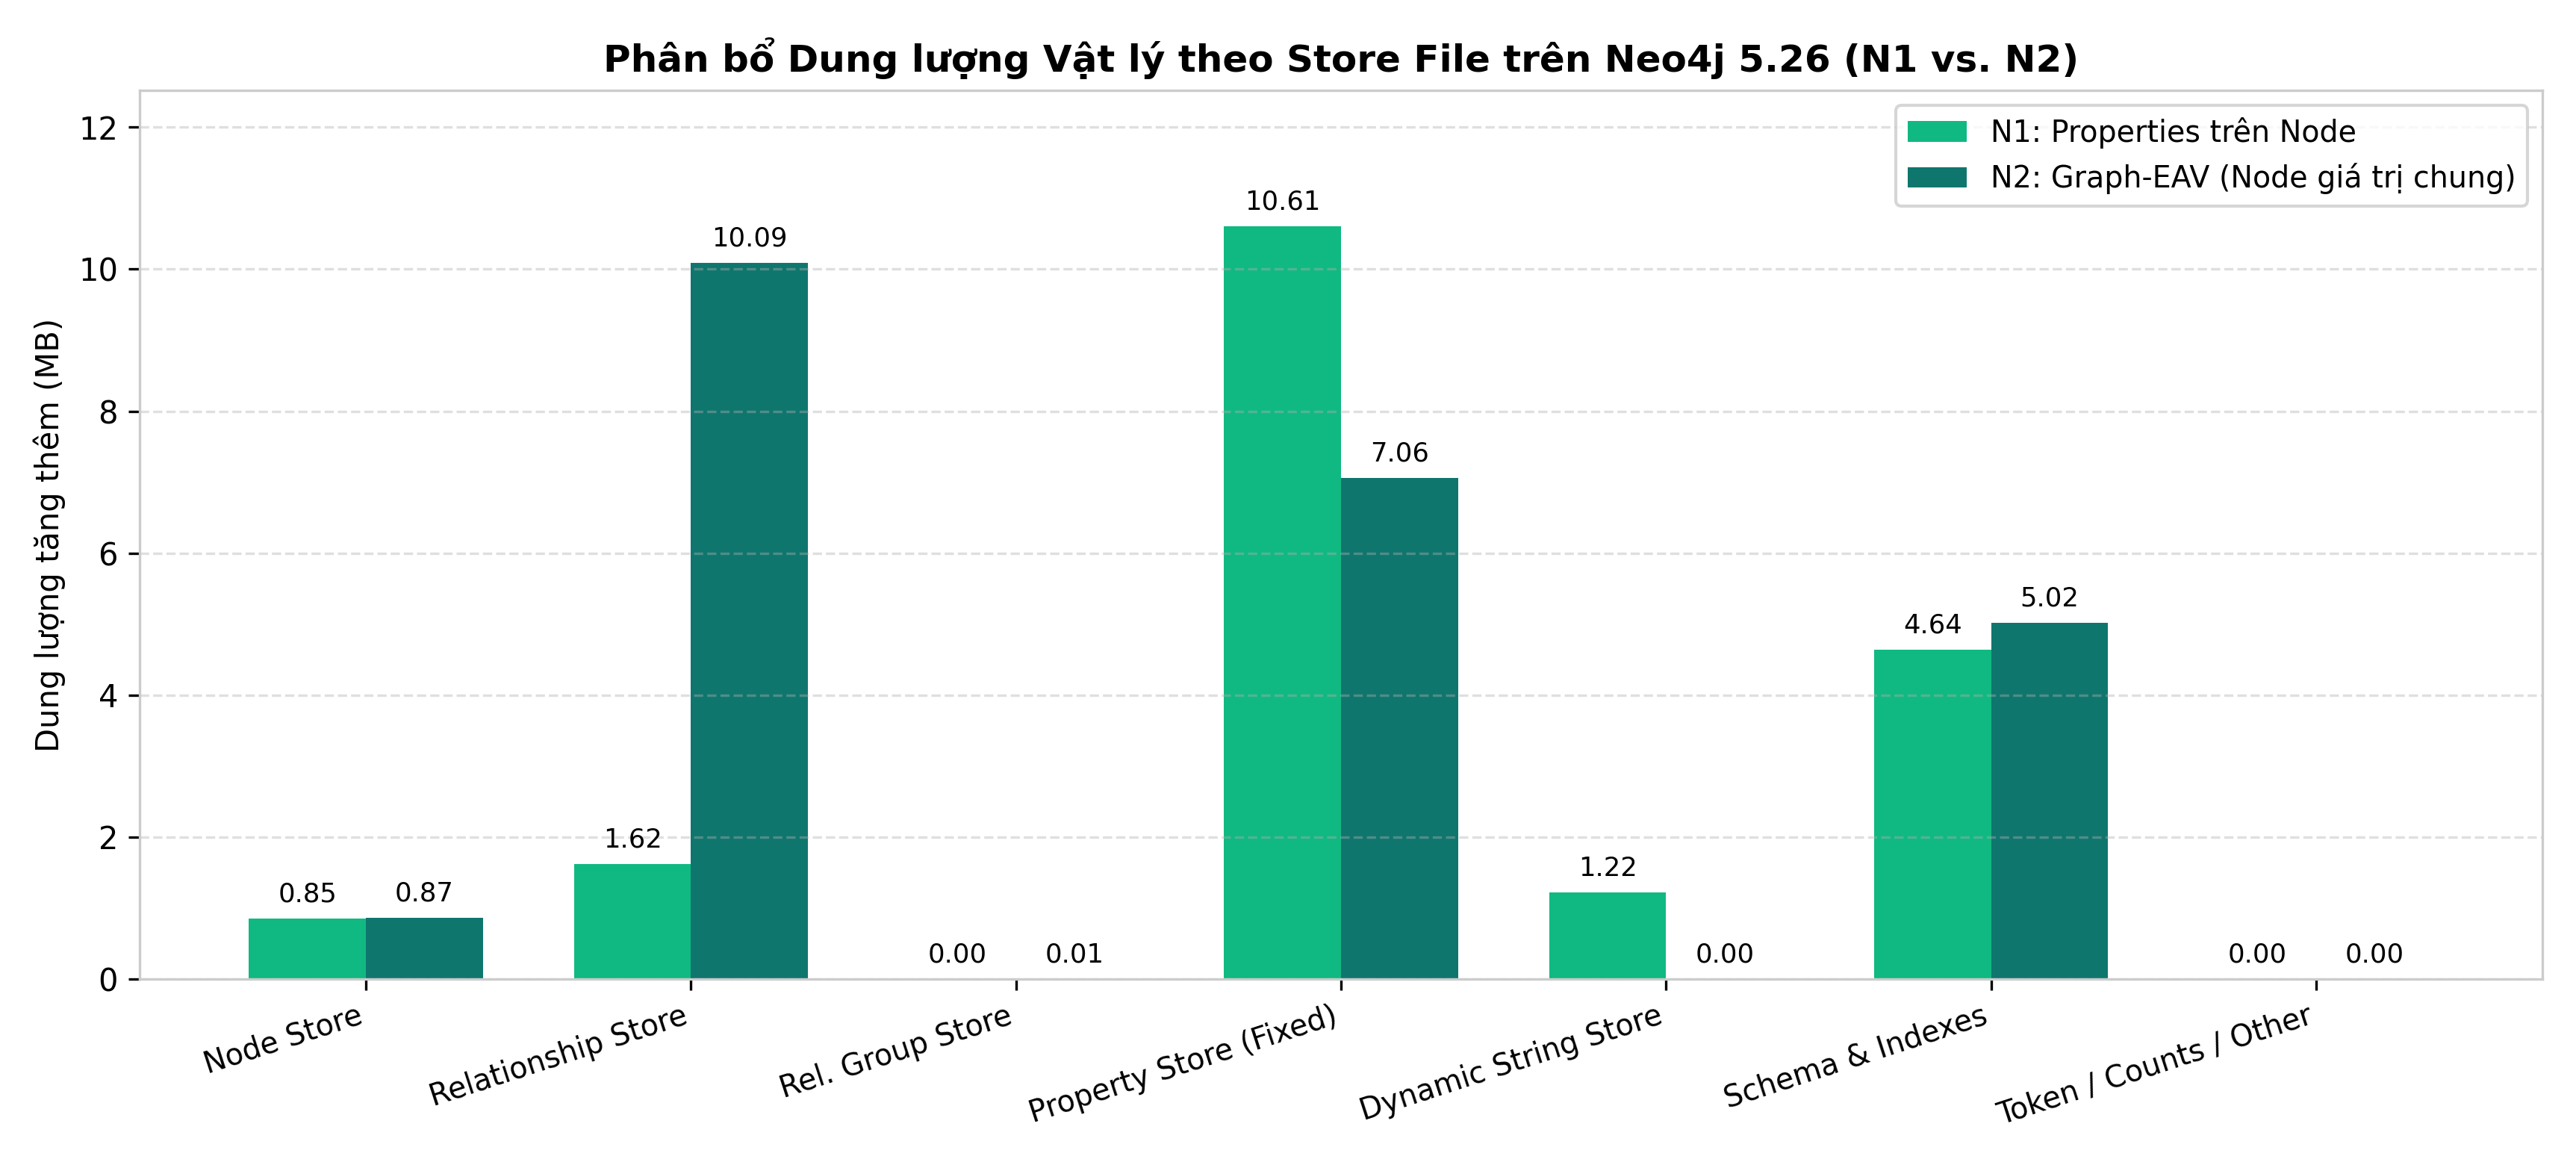
\includegraphics[width=0.95\textwidth]{report/images/topic1_neo4j_store_breakdown.png}
  \caption{Phân bổ dung lượng vật lý theo Store File trên Neo4j 5.26 (N1 vs. N2)}
  \label{fig:t1_neo4j_stores}
\end{figure}

Số liệu đo tại Bảng~\ref{tab:t1_neo4j_stores} và Hình~\ref{fig:t1_neo4j_stores} cho thấy rõ sự dịch chuyển dung lượng giữa các Store File: mô hình \texttt{N1} giữ thuộc tính trên nút làm \texttt{propertystore\_fixed} tăng \textbf{10,61 MB} và \texttt{propertystore\_strings} tăng \textbf{1,22 MB} (do lặp lại 10.000 chuỗi \texttt{isbn\_note}); ngược lại \texttt{N2} (Graph-EAV) triệt tiêu hoàn toàn phần tăng thêm của \texttt{propertystore\_strings} (\textbf{0,00 MB}) nhờ dùng chung nút giá trị, nhưng đẩy mạnh \texttt{relationshipstore} lên \textbf{10,09 MB} để lưu 260.000 cạnh \texttt{[:T1\_HAS\_ATTR]}. Đồng thời, thí nghiệm \textit{Space Reuse} trên 1.000 nút \texttt{:T1DeleteDemo} ghi nhận kích thước tổng trước khi chèn là \textbf{45.457.408 bytes} (\texttt{nodestore = 1.900.544 bytes}), sau khi chèn và checkpoint tăng lên \textbf{46.080.000 bytes} (\texttt{nodestore = 1.916.928 bytes}), và sau khi xóa bằng \texttt{DETACH DELETE} rồi checkpoint lại vẫn giữ mức \textbf{46.096.384 bytes} (\texttt{nodestore = 1.916.928 bytes}), xác nhận tệp vật lý không tự co lại ngay sau khi xóa dữ liệu.

\paragraph{Kịch bản 2: So sánh dung lượng lưu trữ vật lý trên 50.000 biến thể sản phẩm:}
Kịch bản 2 đối chiếu tổng không gian lưu trữ vật lý khi chứa cùng 50.000 biến thể đa ngành hàng giữa 6 mô hình SQL Server (đo từ \texttt{sys.partitions}, \texttt{sys.allocation\_units}, \texttt{sys.dm\_db\_index\_physical\_stats}) và 2 mô hình Neo4j:

\begin{lstlisting}[language=SQL, caption={Trích lược đồ EAV nén PAGE, Native JSON 2025 và SPARSE NULL}, label={lst:t1_sql_models}]
-- M1_EAV_PageComp: EAV value table + covering index with DATA_COMPRESSION = PAGE
CREATE TABLE dbo.T1_Variant_Attr_Values_PageComp (
    variant_id INT NOT NULL, attr_id INT NOT NULL, attr_value NVARCHAR(200) NOT NULL,
    CONSTRAINT PK_T1_EAV_PC PRIMARY KEY CLUSTERED (variant_id, attr_id)
        WITH (DATA_COMPRESSION = PAGE)
);
CREATE NONCLUSTERED INDEX IX_T1_EAV_PC_AttrVal
ON dbo.T1_Variant_Attr_Values_PageComp (attr_id, attr_value)
WITH (DATA_COMPRESSION = PAGE);

-- M2b_JsonNative: Hybrid Relational + Native `json` data type (SQL Server 2025)
CREATE TABLE dbo.T1_Variants_JsonNative (
    variant_id INT NOT NULL PRIMARY KEY CLUSTERED, product_id INT NOT NULL,
    category_name NVARCHAR(30) NOT NULL, sku NVARCHAR(40) NOT NULL,
    price DECIMAL(18,2) NOT NULL, stock_qty INT NOT NULL,
    attributes json NOT NULL
);

-- M3_Sparse: Wide Table with SPARSE NULL columns (0 bytes per NULL value)
CREATE TABLE dbo.T1_Variants_Sparse (
    variant_id INT NOT NULL PRIMARY KEY CLUSTERED, product_id INT NOT NULL,
    category_name NVARCHAR(30) NOT NULL, sku NVARCHAR(40) NOT NULL,
    price DECIMAL(18,2) NOT NULL, stock_qty INT NOT NULL,
    color NVARCHAR(20) NULL, storage_gb INT SPARSE NULL, ram_gb INT SPARSE NULL,
    cpu_model NVARCHAR(40) SPARSE NULL, apparel_size NVARCHAR(10) SPARSE NULL,
    isbn_note NVARCHAR(200) SPARSE NULL -- 20 sparse category columns in total
);
\end{lstlisting}

\begin{table}[htbp]
  \centering
  \scriptsize
  \setlength{\tabcolsep}{3.5pt}
  \renewcommand{\arraystretch}{1.25}
  \setlength{\emergencystretch}{2em}
  \caption{So sánh dung lượng lưu trữ vật lý trên 50.000 biến thể sản phẩm (8 mô hình)}
  \label{tab:t1_storage_50k}
  \begin{tabular}{|p{3.4cm}|p{2.35cm}|p{1.35cm}|p{1.4cm}|p{1.4cm}|p{1.0cm}|p{1.3cm}|}
    \hline
    \textbf{Mô hình lưu trữ} & \textbf{DBMS} & \textbf{Data (MB)} & \textbf{Index (MB)} & \textbf{Total (MB)} & \textbf{B/Var} & \textbf{In-Row Pages} \\
    \hline
    \texttt{M3\_Sparse} (SPARSE)       & SQL Server 2025 & 10,203 &  0,000 & \textbf{10,203} & 214,0 & 1.306 \\ \hline
    \texttt{M1\_EAV\_PageComp}         & SQL Server 2025 &  7,031 &  3,305 & \textbf{10,336} & 216,8 & 1.323 \\ \hline
    \texttt{Control\_WideNoSparse}     & SQL Server 2025 & 10,828 &  0,000 & \textbf{10,828} & 227,1 & 1.386 \\ \hline
    \texttt{M2b\_JsonNative}           & SQL Server 2025 & 14,133 &  0,000 & \textbf{14,133} & 296,4 & 1.809 \\ \hline
    \texttt{M2a\_JsonText}             & SQL Server 2025 & 16,648 &  0,000 & \textbf{16,648} & 349,1 & 2.131 \\ \hline
    \texttt{N1\_Neo4j\_Properties}     & Neo4j 5.26      & 14,305 &  4,641 & \textbf{18,945} & 397,3 & --    \\ \hline
    \texttt{N2\_Neo4j\_GraphEAV}       & Neo4j 5.26      & 18,031 &  5,023 & \textbf{23,055} & 483,5 & --    \\ \hline
    \texttt{M1\_EAV} (Không nén)       & SQL Server 2025 & 13,516 & 11,250 & \textbf{24,766} & 519,4 & 3.170 \\ \hline
  \end{tabular}
\end{table}

\begin{figure}[H]
  \centering
  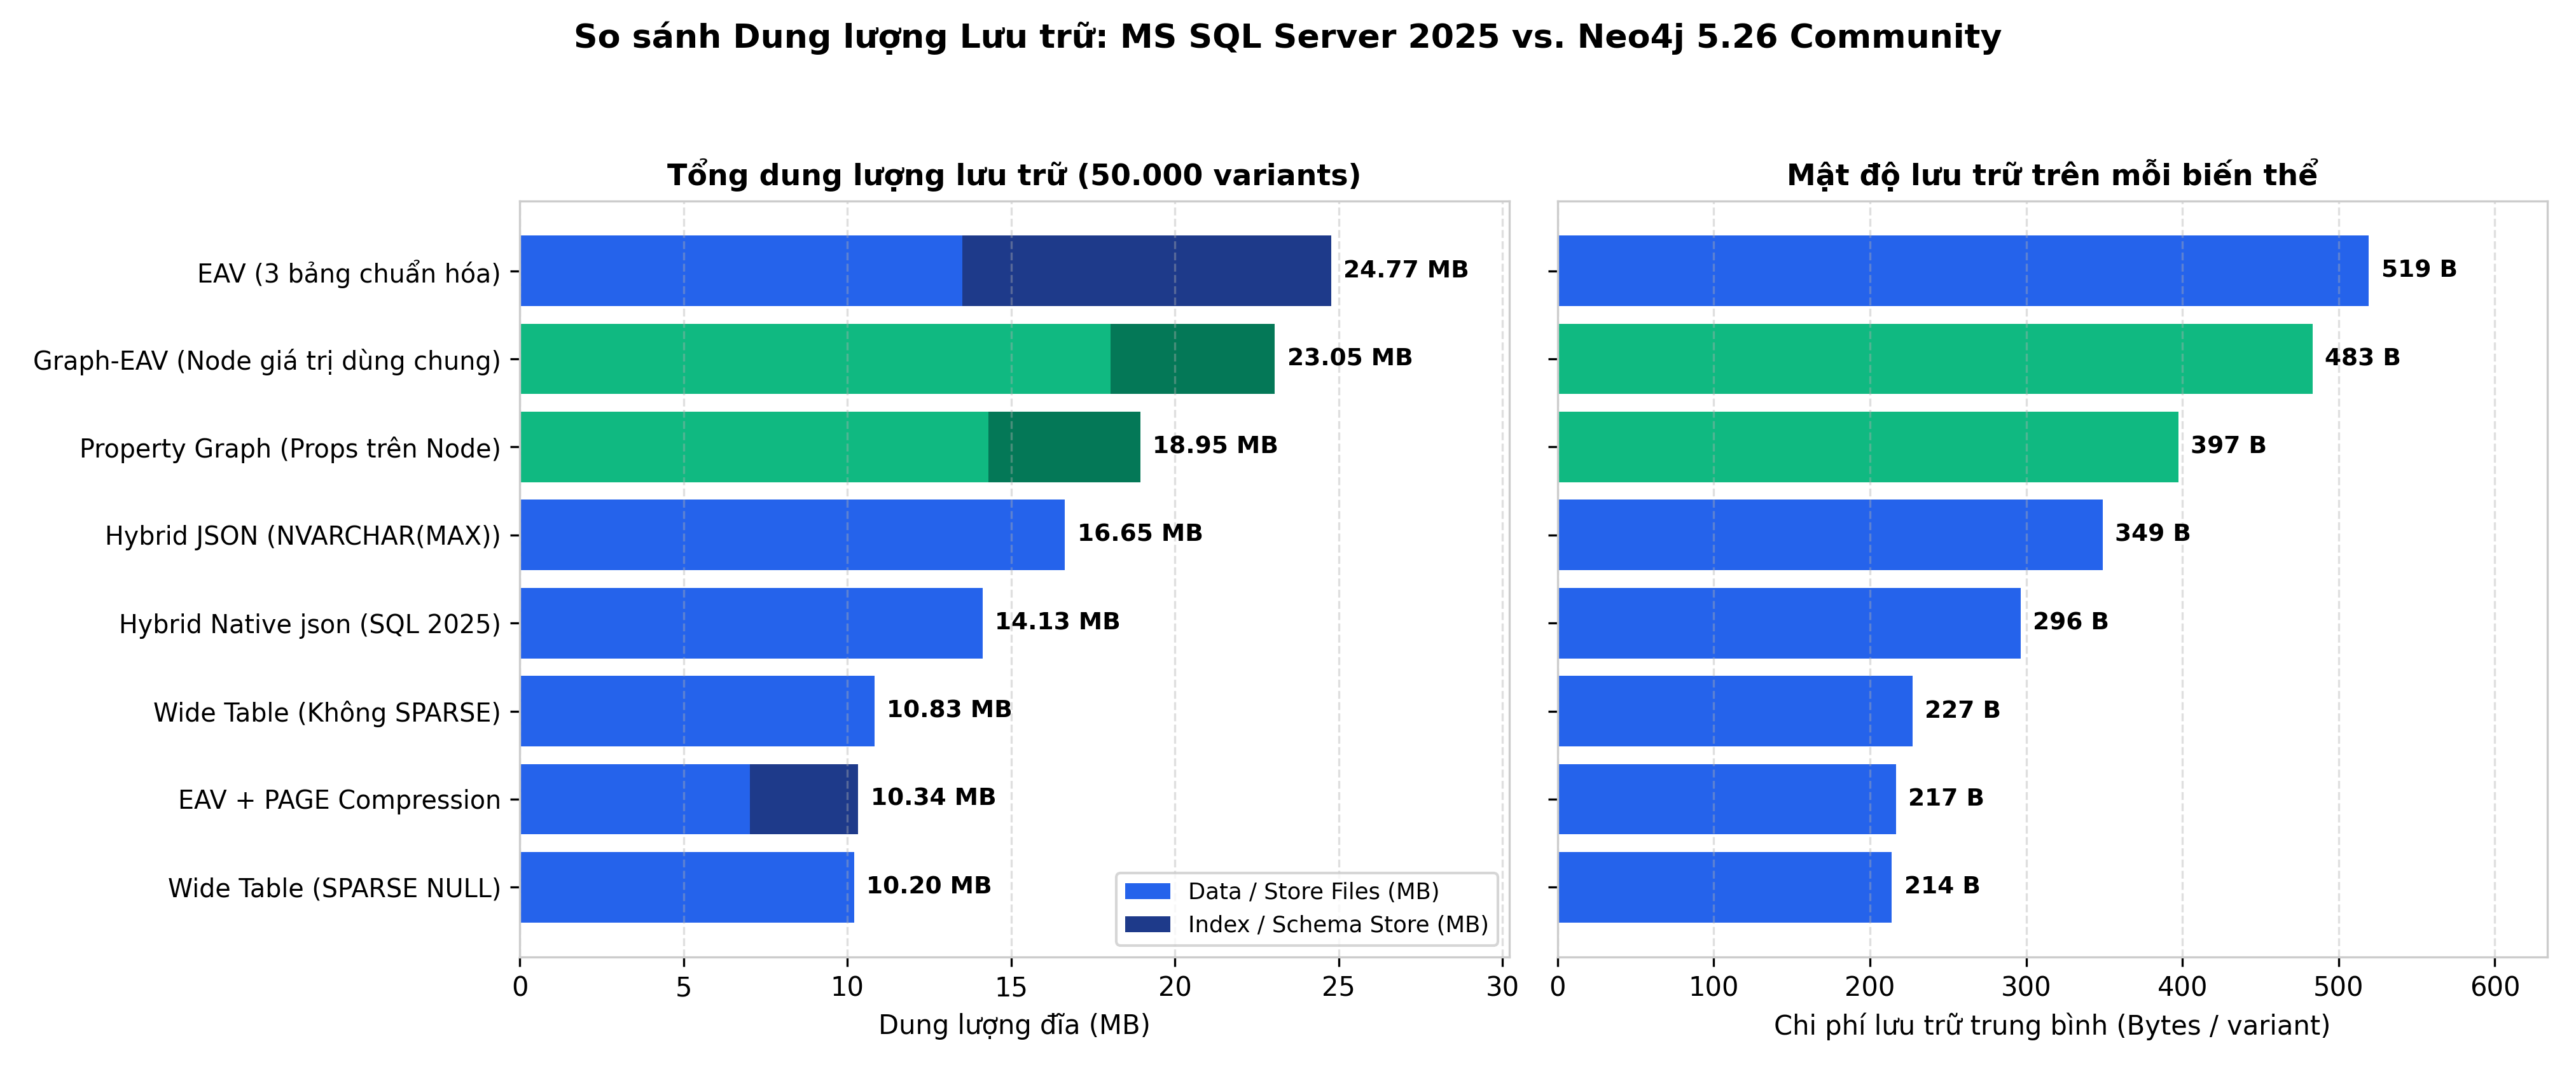
\includegraphics[width=\textwidth]{report/images/topic1_storage_comparison.png}
  \caption{So sánh tổng dung lượng đĩa và mật độ lưu trữ trên mỗi biến thể (50.000 variants)}
  \label{fig:t1_storage_comp}
\end{figure}

Kết quả tại Bảng~\ref{tab:t1_storage_50k} và Hình~\ref{fig:t1_storage_comp} (tất cả bảng SQL đều có 0 trang \texttt{ROW\_OVERFLOW\_DATA} và 0 trang \texttt{LOB\_DATA}) cho thấy bốn điểm nổi bật:
\begin{enumerate}
  \item \textbf{Tác động của nén \texttt{PAGE} lên EAV:} Khi không nén, \texttt{M1\_EAV} tốn nhiều dung lượng nhất (\textbf{24,77 MB}, 519,4 B/biến thể) do nhân thành 260.000 dòng dọc kèm chỉ mục phụ chiếm 11,25 MB. Khi bật \texttt{DATA\_COMPRESSION = PAGE}, nén từ điển và tiền tố nội trang kéo tổng dung lượng giảm \textbf{58,3\%} xuống còn \textbf{10,34 MB} (từ 3.170 xuống 1.323 trang 8 KB).
  \item \textbf{Ưu thế của kiểu \texttt{json} gốc trên SQL Server 2025:} Nhờ lưu nhị phân đã phân tích cú pháp sẵn, \texttt{M2b\_JsonNative} chỉ tiêu tốn \textbf{14,13 MB} (286,37 B/dòng), tiết kiệm trực tiếp \textbf{15,1\%} dung lượng so với \texttt{M2a\_JsonText} lưu văn bản UTF-16 (\textbf{16,65 MB}, 333,79 B/dòng).
  \item \textbf{Hiệu quả thực tế của \texttt{SPARSE NULL}:} Với tỷ lệ \texttt{NULL} 80\% trên 20 cột đặc thù, mô hình \texttt{M3\_Sparse} đạt dung lượng nhỏ nhất (\textbf{10,20 MB}), tiết kiệm \textbf{5,8\%} so với bảng đối chứng \texttt{Control\_WideNoSparse} (\textbf{10,83 MB}) do phần lớn cột chuỗi biến thiên \texttt{NVARCHAR} vốn đã nhỏ gọn khi \texttt{NULL} trong khi cột Sparse phải bù thêm chi phí \textit{Sparse Vector} cho các giá trị khác \texttt{NULL}.
  \item \textbf{Chi phí cấu trúc của Neo4j:} Cả \texttt{N1} (\textbf{18,95 MB}) và \texttt{N2} (\textbf{23,05 MB}) đều lớn hơn các mô hình lai JSON và Sparse của SQL Server vì phải lưu thêm các tệp con trỏ quan hệ hai chiều và chỉ mục nhãn (\texttt{schema\_indexes} chiếm 4,64--5,02 MB).
\end{enumerate}

\paragraph{Kịch bản 3: So sánh khả năng mở rộng Schema (Schema Evolution) và hiệu năng truy vấn (d), (a), (c):}
Kịch bản 3 kiểm tra tốc độ thích ứng khi nghiệp vụ thay đổi và hiệu năng trên nhóm truy vấn thuộc phạm vi Thành viên 1: (1) bổ sung thuộc tính mới \texttt{battery\_mAh = 5000} cho toàn bộ \textbf{10.000 biến thể Smartphones}; (2) chạy \textbf{Truy vấn (d)} điều kiện đơn lọc \texttt{color = 'Black'} (khớp chính xác \textbf{8.000 biến thể} ở cả 8 mô hình, đo trung bình 3 lần sau warmup kèm \texttt{logical reads} / \texttt{PROFILE db hits}); và (3) chạy \textbf{Truy vấn (a)} chèn thuộc tính lạ \texttt{waterproof\_ip = 'IP68'} cùng \textbf{Truy vấn (c)} cập nhật giá và màu cho \texttt{variant\_id = 1}:

\begin{lstlisting}[language=SQL, caption={Thực nghiệm Schema Evolution và truy vấn (d)/(a)/(c) trên MS SQL Server 2025}, label={lst:t1_sql_evo}]
-- 1. Schema Evolution: Wide/Sparse require DDL ALTER TABLE (Sch-M lock)
ALTER TABLE dbo.T1_Variants_Sparse ADD battery_mAh INT SPARSE NULL;
UPDATE dbo.T1_Variants_Sparse
SET battery_mAh = 5000 WHERE category_name = N'Smartphones';

--    Hybrid Native json adds attribute via DML .modify() with ZERO DDL
UPDATE dbo.T1_Variants_JsonNative
SET attributes.modify('$.battery_mAh', 5000)
WHERE category_name = N'Smartphones';

-- 2. Query (d) Single Condition: filter color = 'Black' (8,000 matches)
SELECT COUNT(*) FROM dbo.T1_Variant_Attr_Values_PageComp v
JOIN dbo.T1_Attributes a ON a.attr_id = v.attr_id
WHERE a.attr_name = N'color' AND v.attr_value = N'Black';

SELECT COUNT(*) FROM dbo.T1_Variants_JsonNative
WHERE JSON_VALUE(attributes, '$.color') = N'Black';

-- 3. Query (a) Insert novel attribute & Query (c) Point Update (FR-07)
INSERT INTO dbo.T1_Variants_JsonNative
VALUES (999999, 1, N'Smartphones', N'SKU-DEMO-IP68', 1199.00, 15,
        '{"color":"Black","waterproof_ip":"IP68"}');
UPDATE dbo.T1_Variants_JsonNative
SET price = price + 10.00, attributes.modify('$.color', N'Matte Black')
WHERE variant_id = 1;
\end{lstlisting}

\begin{lstlisting}[language={}, caption={Thực nghiệm Schema Evolution và truy vấn (d)/(a)/(c) trên Neo4j 5}, label={lst:t1_neo_evo}, morekeywords={MATCH,SET,RETURN,count,MERGE,WITH,PROFILE,WHERE,CREATE}, sensitive=false, morecomment={[l]{//}}, morestring={[b]'}]
// 1. Schema Evolution: N1 (SET property, 0 DDL) & N2 (Shared node + 10k edges)
MATCH (v:T1VariantProp {category: 'Smartphones'})
SET v.battery_mAh = 5000 RETURN count(v);

MERGE (a:T1AttrValue {name: 'battery_mAh', value: '5000'})
WITH a MATCH (v:T1VariantGraph {category: 'Smartphones'})
MERGE (v)-[:T1_HAS_ATTR]->(a) RETURN count(v);

// 2. Query (d) Single Condition: LabelScan (N1) vs Index-Free Adjacency (N2)
PROFILE MATCH (v:T1VariantProp) WHERE v.color = 'Black' RETURN count(v);
PROFILE MATCH (:T1AttrValue {name: 'color', value: 'Black'})
              <-[:T1_HAS_ATTR]-(v:T1VariantGraph)
RETURN count(v);

// 3. Query (a) Insert novel property & Query (c) Point Update
MATCH (p:T1Product {product_id: 1})
CREATE (p)-[:T1_HAS_VARIANT]->(:T1VariantProp {
  variant_id: 999999, sku: 'SKU-DEMO-IP68', price: 1199.0,
  color: 'Black', waterproof_ip: 'IP68'
});
MATCH (v:T1VariantProp {variant_id: 1})
SET v.price = v.price + 10.0, v.color = 'Matte Black';
\end{lstlisting}

\begin{table}[htbp]
  \centering
  \scriptsize
  \setlength{\tabcolsep}{3.5pt}
  \renewcommand{\arraystretch}{1.25}
  \setlength{\emergencystretch}{2em}
  \caption{Kết quả thực nghiệm Schema Evolution (10.000 Smartphones) và Truy vấn (d) (8.000 kết quả)}
  \label{tab:t1_evo_query}
  \begin{tabular}{|p{3.3cm}|p{1.2cm}|p{1.1cm}|p{1.9cm}|p{2.4cm}|p{2.1cm}|}
    \hline
    \textbf{Mô hình} & \textbf{Evo (ms)} & \textbf{Qd (ms)} & \textbf{Chi phí đọc} & \textbf{Linh hoạt Schema} & \textbf{An toàn kiểu} \\
    \hline
    \texttt{M1\_EAV}               &   645,12 &          2,03 &     32 \textit{reads} & Cao (Không DDL)         & Yếu (\texttt{NVARCHAR}) \\ \hline
    \texttt{M1\_EAV\_PageComp}     &   737,39 & \textbf{1,06} & \textbf{13 \textit{reads}} & Cao (Không DDL)    & Yếu (\texttt{NVARCHAR}) \\ \hline
    \texttt{M2a\_JsonText}         &   563,72 &        267,00 &  2.887 \textit{reads} & Cao (\texttt{JSON\_\allowbreak MODIFY}) & TB (\texttt{ISJSON}) \\ \hline
    \texttt{M2b\_JsonNative}       &   426,33 &        267,87 &  3.611 \textit{reads} & Cao (\texttt{.modify()}) & TB (Native JSON) \\ \hline
    \texttt{M3\_Sparse}            &   366,21 &         14,84 &  1.904 \textit{reads} & Thấp (DDL \texttt{Sch-M}) & Mạnh (Định kiểu) \\ \hline
    \texttt{Control\_WideNoSparse} &   304,63 &         13,61 &  1.474 \textit{reads} & Thấp (DDL \texttt{Sch-M}) & Mạnh (Định kiểu) \\ \hline
    \texttt{N1\_Neo4j\_Properties} &   758,00 &        123,33 & 100.001 \textit{hits} & Rất cao (0 DDL)         & Yếu (Community) \\ \hline
    \texttt{N2\_Neo4j\_GraphEAV}   & 1.854,00 &         80,33 & 16.004 \textit{hits}  & Rất cao (0 DDL)         & TB (\texttt{AttrValue}) \\ \hline
  \end{tabular}
\end{table}

\begin{figure}[H]
  \centering
  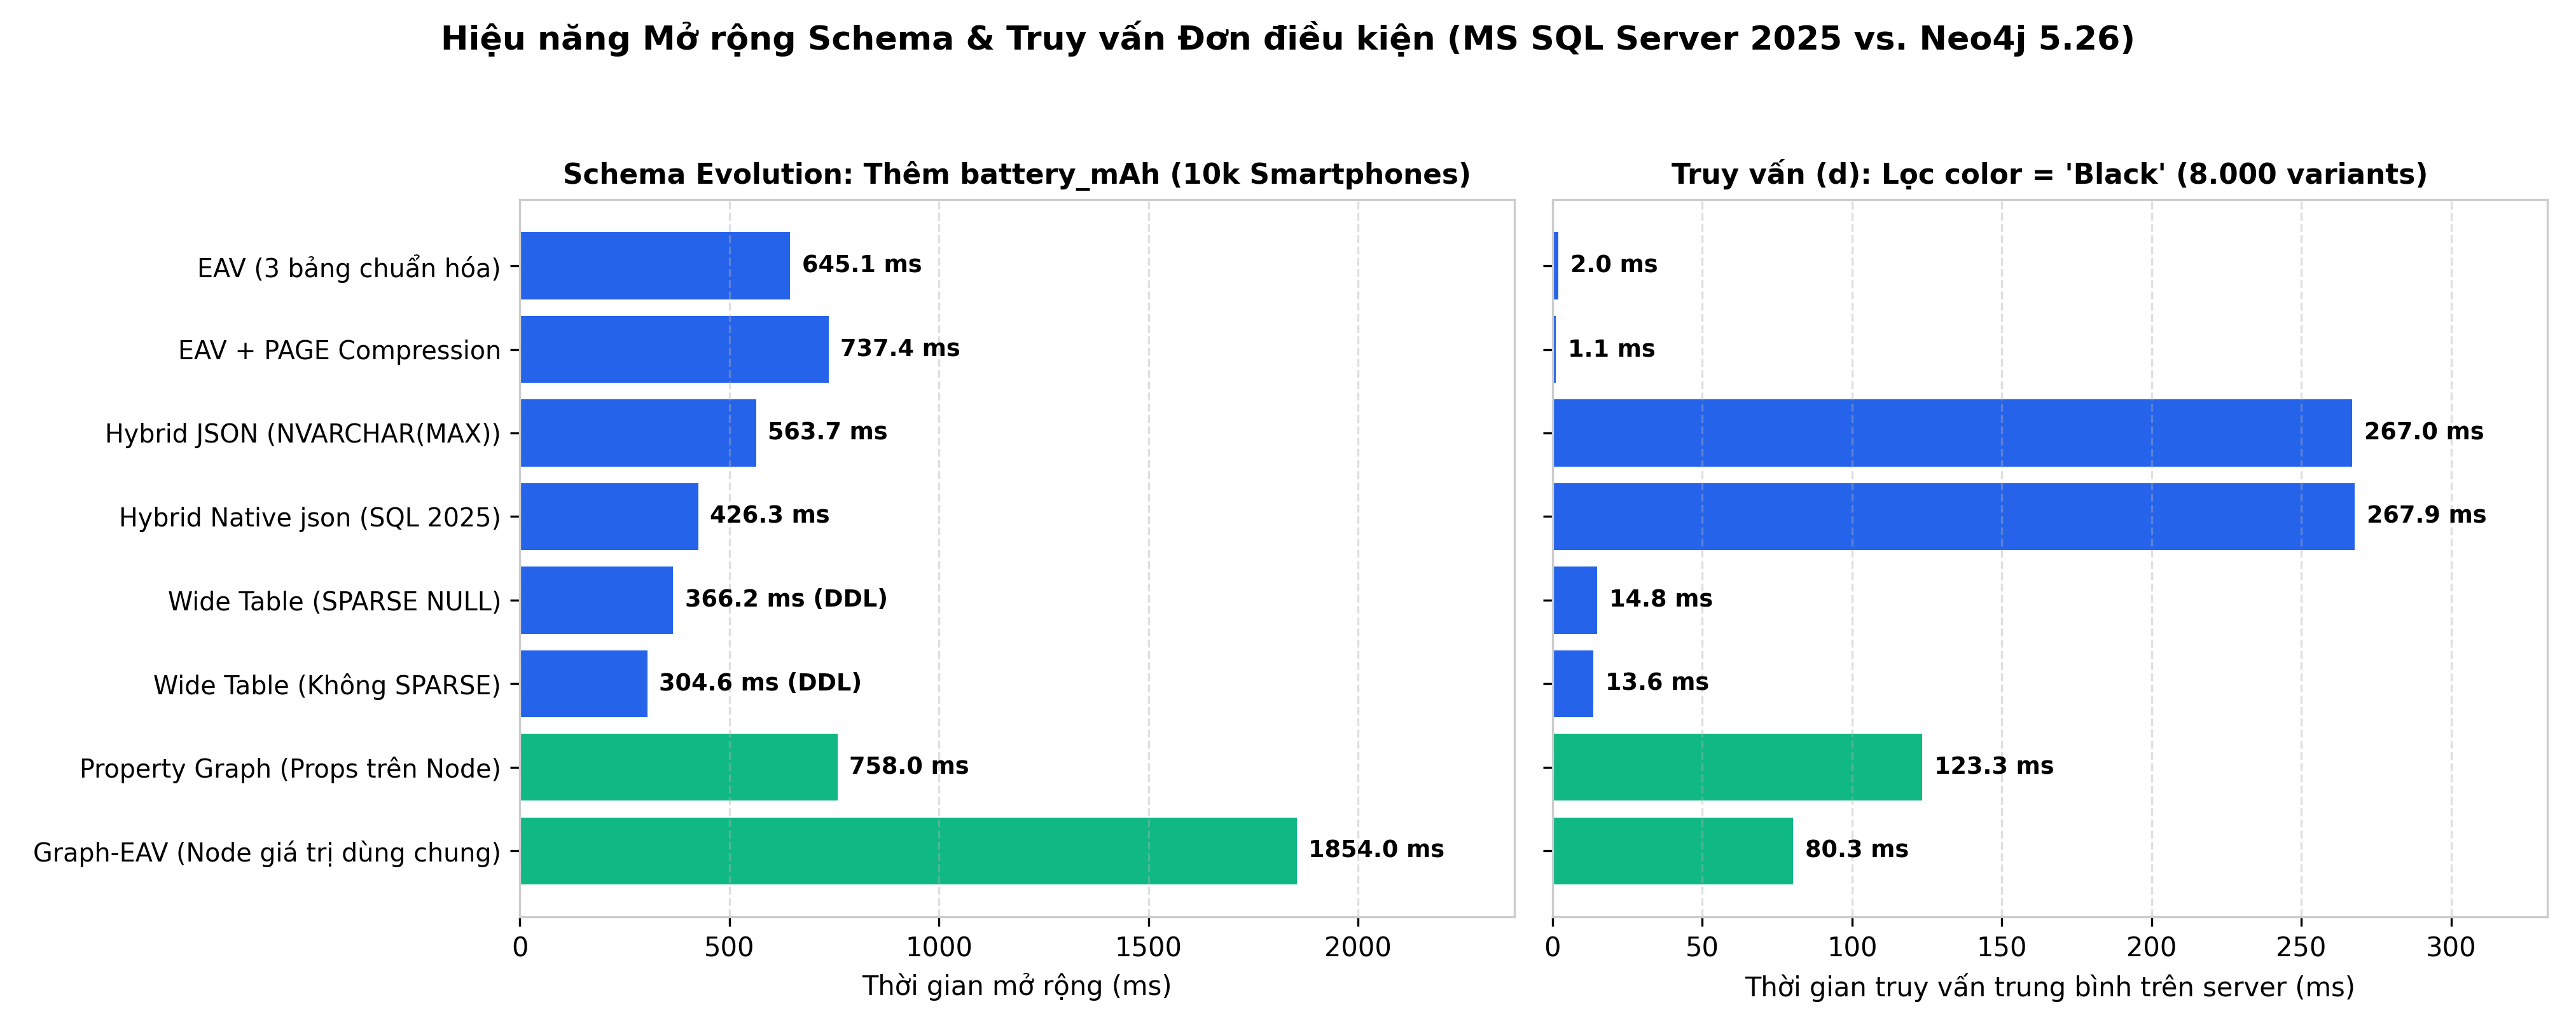
\includegraphics[width=\textwidth]{report/images/topic1_evolution_query.png}
  \caption{Hiệu năng mở rộng Schema và truy vấn đơn điều kiện (MS SQL Server 2025 vs. Neo4j 5.26)}
  \label{fig:t1_evo_query}
\end{figure}

Từ kết quả ở Bảng~\ref{tab:t1_evo_query} và Hình~\ref{fig:t1_evo_query}, có thể phân tích rõ các đánh đổi sau:
\begin{itemize}
  \item \textbf{Mở rộng Schema (\texttt{battery\_mAh}):} Hai bảng rộng \texttt{M3\_Sparse} (366,21 ms) và \texttt{Control\_WideNoSparse} (304,63 ms) phải dùng \texttt{ALTER TABLE} chiếm khóa \textbf{\texttt{Sch-M} (Schema Modification Lock)}, có nguy cơ chặn các giao dịch đồng thời trên hệ thống lớn. Ngược lại, \texttt{M2b\_JsonNative} hoàn tất mở rộng bằng DML \texttt{.modify()} trong \textbf{426,33 ms} (nhanh hơn 24,4\% so với \texttt{JSON\_MODIFY} của \texttt{M2a} ở mức 563,72 ms) mà không cần DDL. Trên Neo4j, \texttt{N1} mở rộng rất gọn bằng \texttt{SET} (758,00 ms), còn \texttt{N2} tốn 1.854,00 ms vì phải tạo mới 10.000 cạnh quan hệ trong \texttt{Relationship Store}.
  \item \textbf{Truy vấn (d) (\texttt{color = 'Black'}):} \texttt{M1\_EAV\_PageComp} đạt tốc độ nhanh nhất (\textbf{1,06 ms}, chỉ \textbf{13 logical reads}) nhờ chỉ mục bao phủ nén \texttt{PAGE}. Hai mô hình JSON chưa tạo chỉ mục computed column phải quét toàn bảng và phân tích JSON nên mất 267,00--267,87 ms. Trên Neo4j, \texttt{N2\_Neo4j\_GraphEAV} (\textbf{80,33 ms}, \textbf{16.004 db hits}) giảm được \textbf{84\% số lần truy cập CSDL} so với \texttt{N1} (\textbf{123,33 ms}, \textbf{100.001 db hits}) do \texttt{N1} phải quét toàn bộ 50.000 nút (\texttt{NodeByLabelScan}), còn \texttt{N2} định vị trực tiếp nút \texttt{:T1AttrValue} và đi theo 8.000 cạnh liền kề bằng \textit{Index-Free Adjacency}.
  \item \textbf{Truy vấn (a) Insert \& (c) Update (FR-07):} Khi thử chèn biến thể mới có thuộc tính lạ \texttt{waterproof\_ip = 'IP68'}, mô hình \texttt{M3\_Sparse} lập tức bị từ chối với lỗi \textbf{Msg 207} (\textit{Invalid column name 'waterproof\_ip'}), thể hiện tính khắt khe của \textit{Schema-on-Write}; trong khi \texttt{M2b\_JsonNative} chèn thành công trong \textbf{5,88 ms} và cập nhật giá + màu cục bộ bằng \texttt{.modify()} chỉ mất \textbf{3,00 ms}. Trên Neo4j, lệnh Cypher đơn lẻ tạo thuộc tính mới kèm dọn dẹp ghi nhận \textbf{669,00 ms} và lệnh cập nhật + khôi phục ghi nhận \textbf{307,00 ms} (do là lượt chạy đơn chưa làm nóng bộ đệm kế hoạch thực thi và bao gồm thao tác dọn dẹp trong cùng phiên \texttt{cypher-shell}).
\end{itemize}

\subsubsection{Đánh giá và quyết định}

Bảng~\ref{tab:t1_summary} tổng hợp các đặc tính cốt lõi về lưu trữ và quản trị dữ liệu giữa MS SQL Server 2025 và Neo4j 5.26:

\begin{table}[htbp]
  \centering
  \footnotesize
  \setlength{\tabcolsep}{4pt}
  \renewcommand{\arraystretch}{1.25}
  \setlength{\emergencystretch}{2em}
  \caption{So sánh tổng hợp cơ chế Data Storage \& Management giữa MS SQL Server và Neo4j}
  \label{tab:t1_summary}
  \begin{tabular}{|p{2.9cm}|p{5.0cm}|p{5.0cm}|}
    \hline
    \textbf{Tiêu chí} & \textbf{MS SQL Server (2025)} & \textbf{Neo4j (5.26 LTS)} \\
    \hline
    Mô hình dữ liệu & Relational Model & Labeled Property Graph \\ \hline
    Thiết kế Schema & Schema-on-Write (ép ràng buộc khi ghi) & Schema-Optional (linh hoạt thuộc tính) \\ \hline
    Tổ chức dữ liệu & Tables, Rows, Columns & Nodes, Relationships, Properties \\ \hline
    Đơn vị lưu trữ & Page 8 KB, Extent 64 KB & Record Store (Aligned) hoặc Block Store \\ \hline
    Cấu trúc lưu trữ & Heap, Clustered Index B+Tree & Node, Relationship, Property Store \\ \hline
    Truy xuất quan hệ & Foreign Key và JOIN & Index-Free Adjacency ($O(1)$/bước nhảy) \\ \hline
    Dữ liệu lớn / động & Row Overflow, LOB, Native \texttt{json}, Sparse & Inline Storage và Dynamic Storage \\ \hline
    Bộ nhớ đệm & Buffer Pool & Off-Heap Page Cache (tách JVM Heap) \\ \hline
    Cơ chế nén & Row Compression, Page Compression & Phụ thuộc Store Format \\ \hline
    Mở rộng thuộc tính & \texttt{ALTER TABLE} (\texttt{Sch-M}) hoặc EAV/JSON & \texttt{SET}/\texttt{CREATE} tức thì (0 DDL) \\ \hline
    Phục hồi dữ liệu & Transaction Log, Checkpoint, REDO/UNDO & Transaction Log, Checkpoint, Recovery \\ \hline
    Thu hồi không gian & Ghost Cleanup, REBUILD, REORGANIZE & Space Reuse và Defragmentation \\ \hline
  \end{tabular}
\end{table}

\paragraph{Quyết định lựa chọn cho hệ thống E-Commerce:} Từ phân tích lý thuyết và số liệu thực nghiệm trên, nhóm quyết định chọn \textbf{MS SQL Server} làm hệ quản trị cơ sở dữ liệu chính cho nền tảng thương mại điện tử đa gian hàng vì ba lý do then chốt:

\begin{enumerate}
  \item \textbf{Bảo toàn tính toàn vẹn bằng Schema-on-Write:} Hệ thống E-Commerce xoay quanh các thực thể giao dịch tài chính và tồn kho (\texttt{Users}, \texttt{Sellers}, \texttt{Products}, \texttt{Orders}, \texttt{Order\_Details}, \texttt{Vouchers}), đòi hỏi cơ chế kiểm tra kiểu dữ liệu, khóa ngoại và ràng buộc \texttt{CHECK} nghiêm ngặt ngay tại tầng Storage Engine (như đã chứng minh bằng lỗi 547 khi chặn giá âm).
  \item \textbf{Hiệu quả nén và lưu trữ đa dạng trên trang 8 KB:} Kiến trúc Page 8 KB kết hợp \texttt{DATA\_COMPRESSION = PAGE} (216,8 B/biến thể) và mô hình lai Native \texttt{json} (296,4 B/biến thể, 0 DDL khi mở rộng) giúp tối ưu dung lượng đĩa vượt trội so với Neo4j (397,3--483,5 B/biến thể), vừa giữ trọn lợi thế quan hệ vừa linh hoạt cho biến thể sản phẩm.
  \item \textbf{Khả năng kết hợp Polyglot Persistence trong tương lai:} Neo4j không phù hợp thay thế cho CSDL giao dịch chính do thiếu chuẩn hóa ràng buộc bảng, nhưng rất lý tưởng để vận hành song song cho các phân hệ phân tích đồ thị nhiều tầng như hệ thống gợi ý sản phẩm cá nhân hóa hoặc phát hiện gian lận liên kết giữa \texttt{Users} -- \texttt{Orders} -- \texttt{Sellers}.
\end{enumerate}


% ==============================================================================
% CÁC ĐOẠN CẦN BỔ SUNG VÀO CÁC VỊ TRÍ KHÁC TRONG main.tex (BỎ COMMENT KHI DÁN)
% ==============================================================================
%
% --- [1] Dòng bổ sung vào Bảng 1 (Danh sách thành viên & Phân công công việc) ---
% 2 & Trần Quốc Hiền & 2310992 &
%   - Nghiên cứu chủ đề Data Storage \& Schema Design (MS SQL Server vs Neo4j) \newline
%   - Thiết kế lược đồ ECommerceDB và hiện thực FR-02, FR-07, AuthModule & 100\% \\ \hline
%
% --- [2] Sửa lỗi tiêu đề "Tài liệu" bị cắt chữ ở cuối main.tex (nếu dùng babel vietnamese) ---
% Thêm dòng này trước \begin{document} trong main.tex:
% \addto\captionsvietnamese{\renewcommand{\refname}{Tài liệu tham khảo}}
%
% --- [3] 9 Tài liệu tham khảo nối tiếp sau [10] trong \begin{thebibliography} ---
% \bibitem{t1_date2004}
% C.~J. Date, \textit{An Introduction to Database Systems}, 8th~ed. Pearson, 2004.
%
% \bibitem{t1_silberschatz2019}
% A.~Silberschatz, H.~F. Korth, and S.~Sudarshan, \textit{Database System Concepts}, 7th~ed. McGraw-Hill, 2019.
%
% \bibitem{t1_delaney2012}
% K.~Delaney et~al., \textit{Microsoft SQL Server 2012 Internals}. Microsoft Press, 2012.
%
% \bibitem{t1_mspages}
% Microsoft Learn, \textit{Pages and Extents Architecture Guide -- SQL Server}. [Online]. Available: \url{https://learn.microsoft.com/en-us/sql/relational-databases/pages-and-extents-architecture-guide}
%
% \bibitem{t1_mssparse}
% Microsoft Learn, \textit{Use Sparse Columns -- SQL Server}. [Online]. Available: \url{https://learn.microsoft.com/en-us/sql/relational-databases/tables/use-sparse-columns}
%
% \bibitem{t1_mscomp}
% Microsoft Learn, \textit{Data Compression -- SQL Server}. [Online]. Available: \url{https://learn.microsoft.com/en-us/sql/relational-databases/data-compression/data-compression}
%
% \bibitem{t1_msnativejson}
% Microsoft Learn, \textit{JSON data type (SQL Server 2025)}. [Online]. Available: \url{https://learn.microsoft.com/en-us/sql/t-sql/data-types/json-data-type}
%
% \bibitem{t1_robinson2015}
% I.~Robinson, J.~Webber, and E.~Eifrem, \textit{Graph Databases: New Opportunities for Connected Data}, 2nd~ed. O'Reilly Media, 2015.
%
% \bibitem{t1_neo4jops}
% Neo4j Documentation, \textit{Operations Manual: Store Formats, Memory Configuration, Transaction Logs and Checkpointing}. [Online]. Available: \url{https://neo4j.com/docs/operations-manual/current/}

%      (hoặc copy-paste toàn bộ nội dung từ \subsubsection{...} đến trước phần
%      comment ở cuối file này).
%   3. Cập nhật Bảng 1 (Danh sách thành viên) và nối các \bibitem{t1_...} ở cuối
%      file này vào khối \begin{thebibliography} của main.tex.
% ==============================================================================

\subsubsection{Khái niệm chung về Data Storage và Data Management}

\textbf{Data Storage (Lưu trữ dữ liệu)} là quá trình tổ chức, cấu trúc hóa và duy trì dữ liệu dưới các định dạng nhị phân phù hợp trên thiết bị lưu trữ thứ cấp (SSD/HDD) nhằm bảo đảm độ bền lâu dài, hiệu quả truy xuất và khả năng mở rộng khi khối lượng dữ liệu gia tăng. Thành phần đảm nhiệm trực tiếp chức năng này bên trong một hệ quản trị cơ sở dữ liệu (DBMS) là \textbf{Storage Engine} -- lớp phần mềm cốt lõi chịu trách nhiệm cấp phát không gian đĩa, quản lý bộ nhớ đệm (\textit{Buffer Pool} hoặc \textit{Page Cache}) và duy trì nhật ký giao dịch (\textit{Transaction Log}) phục vụ khôi phục dữ liệu~\cite{t1_date2004,t1_silberschatz2019}.

\textbf{Data Management (Quản trị dữ liệu)} bao gồm tập hợp các cơ chế vận hành trên dữ liệu đã lưu trữ: kiểm soát toàn vẹn ngữ nghĩa và ràng buộc tham chiếu, thực thi truy vấn, xử lý giao dịch (\textit{Transaction}), điều khiển đồng thời, thu hồi không gian trống và bảo đảm tính bền vững sau sự cố. Kiến trúc lưu trữ ở tầng vật lý ảnh hưởng trực tiếp đến chi phí I/O, hiện tượng phân mảnh trang đĩa, dung lượng lưu trữ tiêu thụ cũng như mức độ linh hoạt khi nghiệp vụ thay đổi.

Trong bài toán thực tế của nhóm là nền tảng sàn thương mại điện tử đa gian hàng (\textit{Multi-Vendor E-Commerce Platform}, CSDL \texttt{ECommerceDB}), hệ thống vừa đòi hỏi tính nhất quán chặt chẽ ở các bảng giao dịch cốt lõi (\texttt{Users}, \texttt{Sellers}, \texttt{Orders}, \texttt{Order\_Details}, \texttt{Vouchers}), vừa phát sinh bài toán đặc trưng về \textbf{thuộc tính biến thể sản phẩm linh hoạt}: sản phẩm thuộc ngành hàng \textit{Smartphones} cần lưu \texttt{storage\_gb}, \texttt{ram\_gb}, \texttt{screen\_inch}, \texttt{chipset}; ngành hàng \textit{Laptops} cần \texttt{cpu\_model}, \texttt{gpu\_model}, \texttt{os\_name}; ngành hàng \textit{Fashion} cần \texttt{apparel\_size}, \texttt{material}, \texttt{fit\_style}; còn ngành hàng \textit{Books} lại cần \texttt{author\_name}, \texttt{publisher}, \texttt{page\_count} và \texttt{isbn\_note}. Cách tiếp cận bài toán này phản ánh rõ sự đối lập giữa hai triết lý thiết kế dữ liệu:

\begin{itemize}
  \item \textbf{MS SQL Server (Schema-on-Write):} Yêu cầu khai báo tường minh toàn bộ cấu trúc bảng, kiểu dữ liệu và các ràng buộc (\texttt{PRIMARY KEY}, \texttt{FOREIGN KEY}, \texttt{CHECK}, \texttt{NOT NULL}, \texttt{UNIQUE}) trước khi ghi dữ liệu. Mọi thao tác \texttt{INSERT} hoặc \texttt{UPDATE} đều được kiểm tra nghiêm ngặt ngay tại thời điểm ghi nhằm bảo đảm tính nhất quán cao.
  \item \textbf{Neo4j (Schema-Optional):} Lưu trữ theo mô hình đồ thị thuộc tính có nhãn (\textit{Labeled Property Graph}), cho phép các nút cùng nhãn mang tập thuộc tính khác nhau và bổ sung thuộc tính mới ngay trong quá trình ghi mà không cần chỉnh sửa lược đồ tĩnh, đồng thời vẫn hỗ trợ \textit{Indexes} và \textit{Constraints} để kiểm soát các khóa định danh quan trọng~\cite{t1_robinson2015,t1_neo4jops}.
\end{itemize}

\subsubsection{Đặc trưng cơ chế Data Storage và Data Management trong MS SQL Server}

\paragraph{Mô hình tổ chức và thiết kế dữ liệu cho thuộc tính động:}
MS SQL Server tổ chức dữ liệu logic dưới dạng bảng hai chiều (\textit{Tables, Rows, Columns}) và cung cấp hai cấu trúc lưu trữ vật lý nền tảng cho dữ liệu hàng (\textit{Rowstore})~\cite{t1_delaney2012,t1_mspages}:
\begin{itemize}
  \item \textbf{Heap:} Bảng không có \textit{Clustered Index}; các dòng dữ liệu được lưu tự do không theo thứ tự khóa và được định vị thông qua địa chỉ vật lý \textbf{RID} (\textit{FileID:PageID:SlotID}).
  \item \textbf{Clustered Index:} Tổ chức bảng dưới dạng cây cân bằng \textbf{B+Tree}, trong đó các nút lá chứa trực tiếp toàn bộ dữ liệu dòng được sắp xếp theo thứ tự khóa cụm (mặc định gắn với \texttt{PRIMARY KEY}).
\end{itemize}

Khi mô hình hóa tập thuộc tính biến thể đa dạng trên nền tảng chuẩn hóa quan hệ (1NF--3NF), các hệ thống dùng SQL Server thường áp dụng một trong ba hướng thiết kế sau:
\begin{itemize}
  \item \textbf{Mô hình Entity--Attribute--Value (EAV):} Tách danh mục thuộc tính sang bảng \texttt{Attributes} và lưu từng cặp thuộc tính--giá trị dưới dạng các dòng dọc trong bảng \texttt{Variant\_Attr\_Values}. EAV cho phép thêm thuộc tính mới bằng lệnh \texttt{INSERT} (không cần DDL), nhưng làm tăng mạnh số dòng dữ liệu, giảm an toàn kiểu dữ liệu (thường phải lưu chuỗi \texttt{NVARCHAR}) và phát sinh nhiều phép \texttt{JOIN} khi truy xuất nhiều thuộc tính cùng lúc.
  \item \textbf{Wide Table với Sparse Columns:} Khai báo tất cả thuộc tính của mọi ngành hàng thành các cột trên một bảng rộng kèm từ khóa \texttt{SPARSE NULL}~\cite{t1_mssparse}. Mỗi giá trị \texttt{NULL} trên cột Sparse tiêu thụ \textbf{0 byte} lưu trữ, nhưng mỗi giá trị khác \texttt{NULL} phát sinh thêm 2--4 byte chi phí quản lý trong cấu trúc \textit{Sparse Vector} (chỉ đạt hiệu quả nén khi tỷ lệ \texttt{NULL} cao, thường $\ge$ 20--40\% tùy kiểu dữ liệu) và vẫn phụ thuộc vào lệnh DDL \texttt{ALTER TABLE} khi cần thêm cột mới.
  \item \textbf{Mô hình Hybrid JSON (\texttt{NVARCHAR(MAX)} và kiểu \texttt{json} gốc trên SQL Server 2025):} Giữ các cột giao dịch cốt lõi (\texttt{variant\_id}, \texttt{product\_id}, \texttt{sku}, \texttt{price}, \texttt{stock\_qty}) dưới dạng quan hệ chuẩn định kiểu chặt chẽ, còn tập thuộc tính đặc thù theo ngành hàng được đóng gói vào cột bán cấu trúc. Trước đây, dữ liệu JSON được lưu dưới dạng chuỗi UTF-16 trong \texttt{NVARCHAR(MAX)} kèm ràng buộc \texttt{CHECK} \texttt{(ISJSON(col) = 1)} và cập nhật qua \texttt{JSON\_MODIFY()}. Từ phiên bản \textbf{MS SQL Server 2025}, hệ thống bổ sung kiểu dữ liệu \textbf{\texttt{json} gốc (Native \texttt{json} Data Type)} lưu ở định dạng nhị phân đã phân tích cú pháp sẵn (\textit{pre-parsed binary}) cùng phương thức \texttt{.modify()} trực tiếp, giúp tiết kiệm dung lượng đĩa và giảm chi phí phân tích cú pháp~\cite{t1_msnativejson}.
\end{itemize}

\paragraph{Kiến trúc tệp và trang lưu trữ (Page \& Extent):}
Ở tầng vật lý, mỗi CSDL SQL Server sử dụng ba loại tệp chính: \texttt{.mdf} (tệp dữ liệu chính), \texttt{.ndf} (tệp dữ liệu phụ) và \texttt{.ldf} (tệp nhật ký giao dịch)~\cite{t1_mspages}. Không gian bên trong tệp dữ liệu được chia nhỏ thành các đơn vị lưu trữ chuẩn hóa~\cite{t1_delaney2012,t1_mspages}:
\begin{itemize}
  \item \textbf{Page:} Đơn vị I/O cơ bản có kích thước cố định \textbf{8 KB (8.192 bytes)}, gồm ba vùng chính: (1) \textit{Page Header} (96 bytes đầu chứa mã trang \texttt{m\_pageId}, loại trang \texttt{m\_type}, số dòng \texttt{m\_slotCnt}, vùng trống \texttt{m\_freeCnt}, số bản ghi ma \texttt{m\_ghostRecCnt} và LSN gần nhất \texttt{m\_lsn}); (2) \textit{Data Area} (nơi lưu nối tiếp các dòng dữ liệu); và (3) \textit{Slot Array} ở cuối trang lưu offset trỏ về vị trí từng dòng theo thứ tự logic.
  \item \textbf{Extent:} Gồm \textbf{8 Page liên tiếp}, tương đương \textbf{64 KB}, gồm \textit{Uniform Extent} (cấp phát cho một đối tượng duy nhất) và \textit{Mixed Extent} (chia sẻ giữa tối đa 8 đối tượng nhỏ).
\end{itemize}

\paragraph{Lưu trữ dữ liệu lớn (Allocation Units) và cơ chế nén:}
SQL Server quản lý dữ liệu có kích thước thay đổi thông qua ba \textbf{Allocation Units}~\cite{t1_mspages}:
\begin{itemize}
  \item \textbf{\texttt{IN\_ROW\_DATA}:} Lưu các cột cố định và biến thiên trực tiếp trên trang dữ liệu chính với giới hạn dòng chuẩn tối đa \textbf{8.060 bytes}.
  \item \textbf{\texttt{ROW\_OVERFLOW\_DATA}:} Tự động đẩy các cột độ dài biến thiên (như \texttt{VARCHAR}, \texttt{NVARCHAR}) sang trang tràn dòng khi tổng kích thước dòng vượt quá 8.060 bytes, giữ lại con trỏ 24-byte trên trang gốc.
  \item \textbf{\texttt{LOB\_DATA}:} Lưu trữ các kiểu dữ liệu khối lớn như \texttt{VARCHAR(MAX)}, \texttt{NVARCHAR(MAX)}, \texttt{VARBINARY\allowbreak(MAX)} hoặc \texttt{json} vượt ngưỡng lưu nội dòng.
\end{itemize}

Để tối ưu dung lượng đĩa và I/O bộ nhớ đệm, SQL Server hỗ trợ hai cơ chế nén tích hợp (\texttt{DATA\_COMPRESSION})~\cite{t1_mscomp}: \textbf{Row Compression} chuyển kiểu dữ liệu cố định sang biểu diễn độ dài biến thiên theo giá trị thực và loại bỏ byte đệm trống; trong khi \textbf{Page Compression} kết hợp tuần tự \textit{Row Compression}, \textit{Prefix Compression} (trích xuất tiền tố chung của cột) và \textit{Dictionary Compression} (thay thế giá trị lặp lại toàn trang bằng từ điển nội trang).

\paragraph{Quản lý không gian, phân mảnh và Transaction Log:}
SQL Server theo dõi không gian cấp phát qua các trang bitmap chuyên biệt gồm \textbf{GAM/SGAM} (trạng thái cấp phát Extent), \textbf{PFS} (tỷ lệ chỗ trống của từng Page) và \textbf{IAM} (ánh xạ các Extent thuộc một Allocation Unit)~\cite{t1_mspages}. Khi thêm, sửa hoặc xóa dữ liệu liên tục, hệ thống có thể phát sinh \textbf{Page Split} (tách đôi trang lá B+Tree đã đầy khi chèn khóa mới), \textbf{Forwarded Record} (dòng trên bảng Heap phình to phải dời sang trang khác để lại con trỏ chuyển tiếp), và \textbf{Ghost Record} (đánh dấu logic bản ghi bị xóa hoặc hủy bỏ trên trang lá để tiến trình nền \textit{Ghost Cleanup} thu hồi sau). Quản trị viên bảo trì cấu trúc bằng \texttt{REORGANIZE}/\texttt{REBUILD} và thu hồi dung lượng tệp đĩa bằng \texttt{DBCC SHRINKFILE}. Toàn bộ biến động trên \textit{Buffer Pool} tuân thủ nguyên tắc \textbf{Write-Ahead Logging (WAL)}, kết hợp tiến trình \textbf{Checkpoint} và cơ chế \textbf{REDO/UNDO} từ Transaction Log để đảm bảo phục hồi bền vững~\cite{t1_delaney2012}.

\subsubsection{Đặc trưng cơ chế Data Storage và Data Management trong Neo4j}

\paragraph{Mô hình Labeled Property Graph:}
Neo4j lưu trữ dữ liệu trực tiếp theo mô hình \textbf{Labeled Property Graph (LPG)} gồm ba thành phần cốt lõi~\cite{t1_robinson2015,t1_neo4jops}:
\begin{itemize}
  \item \textbf{Nodes (Nút):} Đại diện cho thực thể (ví dụ \texttt{:User}, \texttt{:Product}, \texttt{:T1VariantProp}); mỗi nút có thể mang một hoặc nhiều nhãn (\textit{Labels}).
  \item \textbf{Relationships (Quan hệ):} Biểu diễn liên kết có hướng và có kiểu giữa nút nguồn và nút đích, ví dụ \texttt{(User)-[:PLACED]->(Order)} hay \texttt{(Product)-\allowbreak[:HAS\_VARIANT]->\allowbreak(Variant)}; mỗi cạnh cũng có thể mang thuộc tính riêng.
  \item \textbf{Properties (Thuộc tính):} Các cặp \textit{Key--Value} linh hoạt gắn trực tiếp lên Node hoặc Relationship.
\end{itemize}

\paragraph{Native Graph Storage và Index-Free Adjacency:}
Neo4j tổ chức dữ liệu đồ thị gốc thành các tệp store vật lý chuyên biệt có kích thước bản ghi cố định trong thư mục dữ liệu~\cite{t1_neo4jops}:
\begin{itemize}
  \item \textbf{Node Store (\texttt{neostore.nodestore.db}):} Lưu thông tin nút, nhãn và con trỏ trỏ tới quan hệ đầu tiên cùng chuỗi thuộc tính đầu tiên.
  \item \textbf{Relationship Store (\texttt{neostore.relationshipstore.db}):} Lưu nút nguồn, nút đích, loại quan hệ và chuỗi liên kết đôi đến các quan hệ kế tiếp của hai đầu nút.
  \item \textbf{Relationship Group Store (\texttt{neostore.\allowbreak relationshipgroupstore.db}):} Gom nhóm cạnh theo loại và chiều đối với các \textit{dense nodes} (nút có mật độ kết nối lớn).
  \item \textbf{Property Store (\texttt{neostore.propertystore.db}) \& Dynamic Store:} Lưu bản ghi thuộc tính cố định và tham chiếu đến vùng lưu trữ động.
\end{itemize}

Neo4j hỗ trợ nhiều \textbf{Store Format} khác nhau theo phiên bản và ấn bản: \textit{Aligned Format} là định dạng mặc định trên ấn bản Community Edition (tối ưu sắp thẳng biên trang với kích thước bản ghi nhẹ), trong khi \textit{Block Format} được sử dụng mặc định trên các phiên bản Enterprise Edition tương ứng~\cite{t1_neo4jops}. Nhờ lưu trực tiếp con trỏ cạnh ngay tại mỗi nút, Neo4j đạt được cơ chế \textbf{Index-Free Adjacency}: hệ thống duyệt qua các mối liên kết lân cận theo tham chiếu trực tiếp với chi phí $O(1)$ cho mỗi bước nhảy mà không cần tra cứu chỉ mục toàn cục như phép \texttt{JOIN} trong SQL Server~\cite{t1_robinson2015}. Tuy nhiên, nếu truy vấn lọc thuộc tính trên toàn bộ nút mà không qua cạnh hoặc chỉ mục, Neo4j vẫn phải quét nhãn (\texttt{NodeByLabelScan}).

\paragraph{Lưu trữ thuộc tính động, Page Cache và Transaction Log:}
Để cân bằng tốc độ truy cập và kích thước thuộc tính biến thiên, Neo4j kết hợp hai cơ chế lưu thuộc tính~\cite{t1_neo4jops}:
\begin{itemize}
  \item \textbf{Inline Storage:} Các giá trị nguyên thủy và chuỗi ngắn vừa kích thước khối thuộc tính được mã hóa và lưu trực tiếp trong \texttt{Property Store}, hạn chế đọc thêm tệp ngoài.
  \item \textbf{Dynamic Storage:} Các chuỗi dài hoặc mảng lớn vượt ngưỡng được tách sang tệp lưu trữ động (\texttt{.strings}, \texttt{.arrays}) và tham chiếu ngược từ bản ghi chính.
\end{itemize}

Về quản lý bộ nhớ và không gian đĩa, Neo4j sử dụng \textbf{Off-Heap Page Cache} (vùng nhớ Native Memory tách biệt khỏi JVM Heap) để lưu đệm các trang store và chỉ mục, qua đó tránh áp lực tạm dừng dọn rác (\textit{Garbage Collection pauses}). Khi dữ liệu bị xóa, các vị trí ID được giải phóng vào tệp \texttt{*.id} để tái sử dụng (\textbf{Space Reuse}) cho lần ghi mới; kích thước tệp vật lý trên đĩa không tự động thu gọn ngay sau khi xóa mà đòi hỏi công cụ bảo trì ngoại tuyến phù hợp theo phiên bản. Tương tự SQL Server, mọi giao dịch thay đổi đồ thị được ghi tuần tự vào \textbf{Transaction Log} và ép đồng bộ trước khi commit, kết hợp \textbf{Checkpoint} xả thay đổi từ Page Cache xuống Store Files nhằm bảo đảm tính bền vững và khả năng phục hồi sau sự cố~\cite{t1_neo4jops}.

\subsubsection{Kịch bản so sánh thực tế giữa MS SQL Server và Neo4j}

\paragraph{Thiết lập môi trường và bộ dữ liệu thực nghiệm:}
Phần thực nghiệm chuyên sâu Chủ đề 1 được triển khai trên \textbf{MS SQL Server 2025 (RTM 17.0.1000.7 -- Enterprise Developer Edition)} để kiểm chứng kiến trúc trang 8 KB trên CSDL \texttt{ECommerceDB} (song song với môi trường Docker MS SQL Server 2022 trình bày ở Mục 4.4 và 5.2) và đánh giá đầy đủ các mô hình lưu trữ biến thể (bao gồm kiểu \texttt{json} gốc mới của SQL Server 2025) trong CSDL cô lập \texttt{Topic1\_StorageLab}, đối chiếu trực tiếp với \textbf{Neo4j 5.26 Community LTS} (container \texttt{ecommerce\_neo4j}, Aligned Store Format, tách riêng nhãn \texttt{T1*} để bảo toàn nguyên vẹn đồ thị mẫu ban đầu).

Nhóm sinh tất định \textbf{10.000 sản phẩm $\times$ 5 biến thể = 50.000 biến thể} thuộc 5 ngành hàng (\textit{Smartphones}, \textit{Laptops}, \textit{Fashion}, \textit{Home\_Living}, \textit{Books}) với \textbf{21 thuộc tính} chuyên biệt (tỷ lệ \texttt{NULL} trên 20 thuộc tính đặc thù đạt 80\%; thuộc tính \texttt{color} có 8.000 biến thể mang giá trị \texttt{'Black'}) và triển khai trên \textbf{8 mô hình}:
\begin{enumerate}
  \item \texttt{M1\_EAV}: EAV 3 bảng chuẩn hóa (260.000 dòng thuộc tính + nonclustered index).
  \item \texttt{M1\_EAV\_PageComp}: Tương tự \texttt{M1\_EAV} nhưng bật \texttt{DATA\_COMPRESSION = PAGE}.
  \item \texttt{M2a\_JsonText}: Mô hình lai giữa bảng quan hệ và cột \texttt{attributes} kiểu \texttt{NVARCHAR(MAX)} có \texttt{CHECK (ISJSON = 1)}.
  \item \texttt{M2b\_JsonNative}: Hybrid Relational + kiểu \texttt{attributes json} gốc (SQL Server 2025).
  \item \texttt{M3\_Sparse}: Wide Table khai báo 20 cột đặc thù dạng \texttt{SPARSE NULL}.
  \item \texttt{Control\_WideNoSparse}: Wide Table đối chứng không có từ khóa \texttt{SPARSE}.
  \item \texttt{N1\_Neo4j\_Properties}: Lưu thuộc tính trực tiếp trên nút \texttt{:T1VariantProp} dưới dạng cặp khóa--giá trị (\textit{Key--Value}).
  \item \texttt{N2\_Neo4j\_GraphEAV}: Chuẩn hóa thành nút giá trị dùng chung \texttt{:T1AttrValue} nối với \texttt{:T1VariantGraph} qua 260.000 cạnh \texttt{[:T1\_HAS\_ATTR]}.
\end{enumerate}

\paragraph{Kịch bản 1: Kiểm chứng Schema-on-Write vs. Schema-Optional và kiến trúc lưu trữ vật lý:}
Kịch bản 1 kiểm chứng cơ chế ép ràng buộc ngay khi ghi trên \texttt{ECommerceDB}, đồng thời giải phẫu trang dữ liệu 8 KB và các tệp store vật lý của Neo4j. Trên MS SQL Server, tập lệnh \texttt{05\_page\_internals.sql} thực hiện chèn một sản phẩm có giá âm (\texttt{-5.00}) vào bảng \texttt{dbo.Products}, thống kê các Allocation Units và đọc trực tiếp cấu trúc trang bằng \texttt{DBCC IND} và \texttt{DBCC PAGE}:

\begin{lstlisting}[language=SQL, caption={Kiểm chứng Schema-on-Write và giải phẫu trang 8 KB trên ECommerceDB}, label={lst:t1_page_internals}]
USE [ECommerceDB];
GO
-- 1. Schema-on-Write: CK_Products_price rejects negative price
BEGIN TRY
    INSERT INTO dbo.Products (seller_id, category_id, name, price)
    VALUES (1, 2, N'Topic1 Schema-on-Write Test', -5.00);
END TRY
BEGIN CATCH
    SELECT ERROR_NUMBER() AS error_number, ERROR_SEVERITY() AS severity,
           ERROR_MESSAGE() AS error_message;
END CATCH;

-- 2. Inspect Allocation Units across 9 ECommerceDB tables (1 page = 8 KB)
SELECT t.name AS table_name,
       MAX(CASE WHEN i.index_id IN (0, 1) THEN p.rows ELSE 0 END) AS row_count,
       SUM(au.total_pages) AS total_pages_8kb,
       SUM(au.used_pages) AS used_pages_8kb,
       CAST(SUM(au.used_pages) * 8.0 AS DECIMAL(10, 2)) AS used_kb
FROM sys.tables t
JOIN sys.indexes i ON t.object_id = i.object_id
JOIN sys.partitions p ON i.object_id = p.object_id AND i.index_id = p.index_id
JOIN sys.allocation_units au ON p.partition_id = au.container_id
GROUP BY t.name ORDER BY used_pages_8kb DESC;

-- 3. Physical 8 KB Page Anatomy of dbo.Products
DBCC TRACEON(3604);
DBCC IND('ECommerceDB', 'dbo.Products', 1);
DBCC PAGE('ECommerceDB', 1, 472, 3);
DBCC TRACEOFF(3604);
\end{lstlisting}

\begin{lstlisting}[language={}, numbers=none, caption={Kết quả thực thi Schema-on-Write và DBCC PAGE (1:472) trên ECommerceDB}, label={lst:t1_page_out}, keywordstyle={}, commentstyle={}, stringstyle={}]
error_number|severity|error_message
547|16|The INSERT statement conflicted with the CHECK constraint "CK_Products_price".
       The conflict occurred in database "ECommerceDB", table "dbo.Products",
       column 'price'.

DBCC IND: Page (1:444) [PageType=10, IAM] | Page (1:472) [PageType=1, IndexLevel=0]
PAGE HEADER (1:472):
  m_pageId = (1:472)   m_type = 1    pminlen = 50    m_slotCnt = 25
  m_freeCnt = 620      m_freeData = 7778             m_lsn = (45:342:13)
  m_ghostRecCnt = 1    GAM (1:2) = ALLOCATED         PFS (1:1) = 0x48 ALLOCATED
Slot 0  Offset 0x60   Length 298 | Record Type = PRIMARY_RECORD
  product_id = 1 | name = iPhone 15 Pro Max 256GB Natural Titanium | price = 1199.00
Slot 24 Offset 0x1de2 Length 128 | Record Type = GHOST_DATA_RECORD
  product_id = 27 | name = Topic1 Schema-on-Write Test | price = -5.00
\end{lstlisting}

\begin{table}[htbp]
  \centering
  \footnotesize
  \setlength{\tabcolsep}{4pt}
  \renewcommand{\arraystretch}{1.25}
  \caption{Phân bổ trang 8 KB và Allocation Units trên 9 bảng của \texttt{ECommerceDB}}
  \label{tab:t1_ecommercedb_pages}
  \begin{tabular}{|p{3.0cm}|p{1.5cm}|p{2.1cm}|p{2.1cm}|p{2.1cm}|p{2.1cm}|}
    \hline
    \textbf{Tên bảng} & \textbf{Số dòng} & \textbf{Total Pages} & \textbf{Used Pages} & \textbf{In-Row Pages} & \textbf{Used (KB)} \\
    \hline
    \texttt{Order\_Details} & 22 & 36 & 8 & 8 & 64.00 \\ \hline
    \texttt{Orders}         & 16 & 36 & 8 & 8 & 64.00 \\ \hline
    \texttt{Products}       & 24 & 36 & 8 & 8 & 64.00 \\ \hline
    \texttt{Reviews}        & 16 & 36 & 8 & 8 & 64.00 \\ \hline
    \texttt{Sellers}        &  5 & 27 & 6 & 6 & 48.00 \\ \hline
    \texttt{Users}          & 14 & 27 & 6 & 6 & 48.00 \\ \hline
    \texttt{Cart\_Items}    & 12 & 18 & 4 & 4 & 32.00 \\ \hline
    \texttt{Categories}     &  8 & 18 & 4 & 4 & 32.00 \\ \hline
    \texttt{Vouchers}       &  6 &  9 & 2 & 2 & 16.00 \\ \hline
  \end{tabular}
\end{table}

Kết quả tại Listing~\ref{lst:t1_page_out} và Bảng~\ref{tab:t1_ecommercedb_pages} chứng minh rõ hai cơ chế lõi của SQL Server: (1) Ràng buộc \texttt{CK\_Products\_price} từ chối ngay bản ghi giá âm với mã lỗi \textbf{547}, đồng thời bản ghi bị hủy vẫn hiện diện ở \texttt{Slot 24} dưới dạng \texttt{GHOST\_DATA\_RECORD} (\texttt{m\_ghostRecCnt = 1}) minh họa trực tiếp cơ chế \textit{Ghost Record} chờ thu hồi nền; (2) Toàn bộ 24 sản phẩm hiện hữu của \texttt{dbo.Products} nằm gọn trong 8 trang \texttt{IN\_ROW\_DATA} (64.00 KB), cột \texttt{NVARCHAR(MAX)} (\texttt{description}, 144 bytes) được nhúng nội dòng (\textit{BLOB Inline Data}) và trạng thái cấp phát được quản lý qua \texttt{GAM (1:2)}, \texttt{PFS (1:1)} cùng trang \texttt{IAM (1:444)}.

Trên Neo4j 5.26 Community, nhóm kiểm chứng tính \textit{Schema-Optional} bằng cách tạo 3 nút cùng nhãn \texttt{:T1DemoItem} nhưng mang bộ thuộc tính hoàn toàn khác nhau, đồng thời thực hiện thí nghiệm \textit{Space Reuse} với 1.000 nút đệm \texttt{:T1DeleteDemo}:

\begin{lstlisting}[language={}, caption={Kiểm chứng Schema-Optional và thí nghiệm Space Reuse trên Neo4j 5}, label={lst:t1_neo_demo}, morekeywords={CREATE,UNWIND,range,toString,MATCH,DETACH,DELETE}, sensitive=false, morecomment={[l]{//}}, morestring={[b]'}]
// 1. Schema-Optional: 3 nodes with same label, heterogeneous property sets
CREATE
  (:T1DemoItem {name: 'iPhone 15 Pro Max', color: 'Natural Titanium',
                storage: '256GB'}),
  (:T1DemoItem {name: 'Men Oxford Shirt', size: 'L', color: 'Light Blue'}),
  (:T1DemoItem {name: 'Clean Code', author: 'Robert C. Martin', pages: 464});

// 2. Space Reuse: insert 1,000 nodes -> restart -> DETACH DELETE -> restart
UNWIND range(1, 1000) AS i
CREATE (:T1DeleteDemo {
  id: i, pad: 'SpaceReuseDemoPayload_0123456789_' + toString(i)
});
MATCH (d:T1DeleteDemo) DETACH DELETE d;
\end{lstlisting}

\begin{table}[htbp]
  \centering
  \footnotesize
  \setlength{\tabcolsep}{4pt}
  \renewcommand{\arraystretch}{1.25}
  \setlength{\emergencystretch}{2em}
  \caption{Phân bổ dung lượng tăng thêm theo từng Store File trên Neo4j 5.26 (N1 vs. N2)}
  \label{tab:t1_neo4j_stores}
  \begin{tabular}{|p{5.2cm}|p{1.9cm}|p{1.5cm}|p{1.9cm}|p{1.5cm}|}
    \hline
    \textbf{Nhóm tệp vật lý (Store Bucket)} & \textbf{N1 Delta (B)} & \textbf{N1 (MB)} & \textbf{N2 Delta (B)} & \textbf{N2 (MB)} \\
    \hline
    Node Store (\texttt{nodestore.db})               &    892.928 &  0,8516 &    909.312 &  0,8672 \\ \hline
    Relationship Store (\texttt{relationshipstore})  &  1.703.936 &  1,6250 & 10.584.064 & 10,0938 \\ \hline
    Rel. Group Store (\texttt{relationshipgroup})    &          0 &  0,0000 &      8.192 &  0,0078 \\ \hline
    Property Store Fixed (\texttt{propertystore.db}) & 11.124.736 & 10,6094 &  7.405.568 &  7,0625 \\ \hline
    Dynamic String Store (\texttt{.strings})         &  1.277.952 &  1,2188 &          0 &  0,0000 \\ \hline
    Schema \& Indexes (\texttt{schema/})             &  4.866.048 &  4,6406 &  5.267.456 &  5,0234 \\ \hline
    \textbf{Tổng cộng (50.000 variants)}             & \textbf{19.865.600} & \textbf{18,9453} & \textbf{24.174.592} & \textbf{23,0547} \\ \hline
  \end{tabular}
\end{table}

\begin{figure}[H]
  \centering
  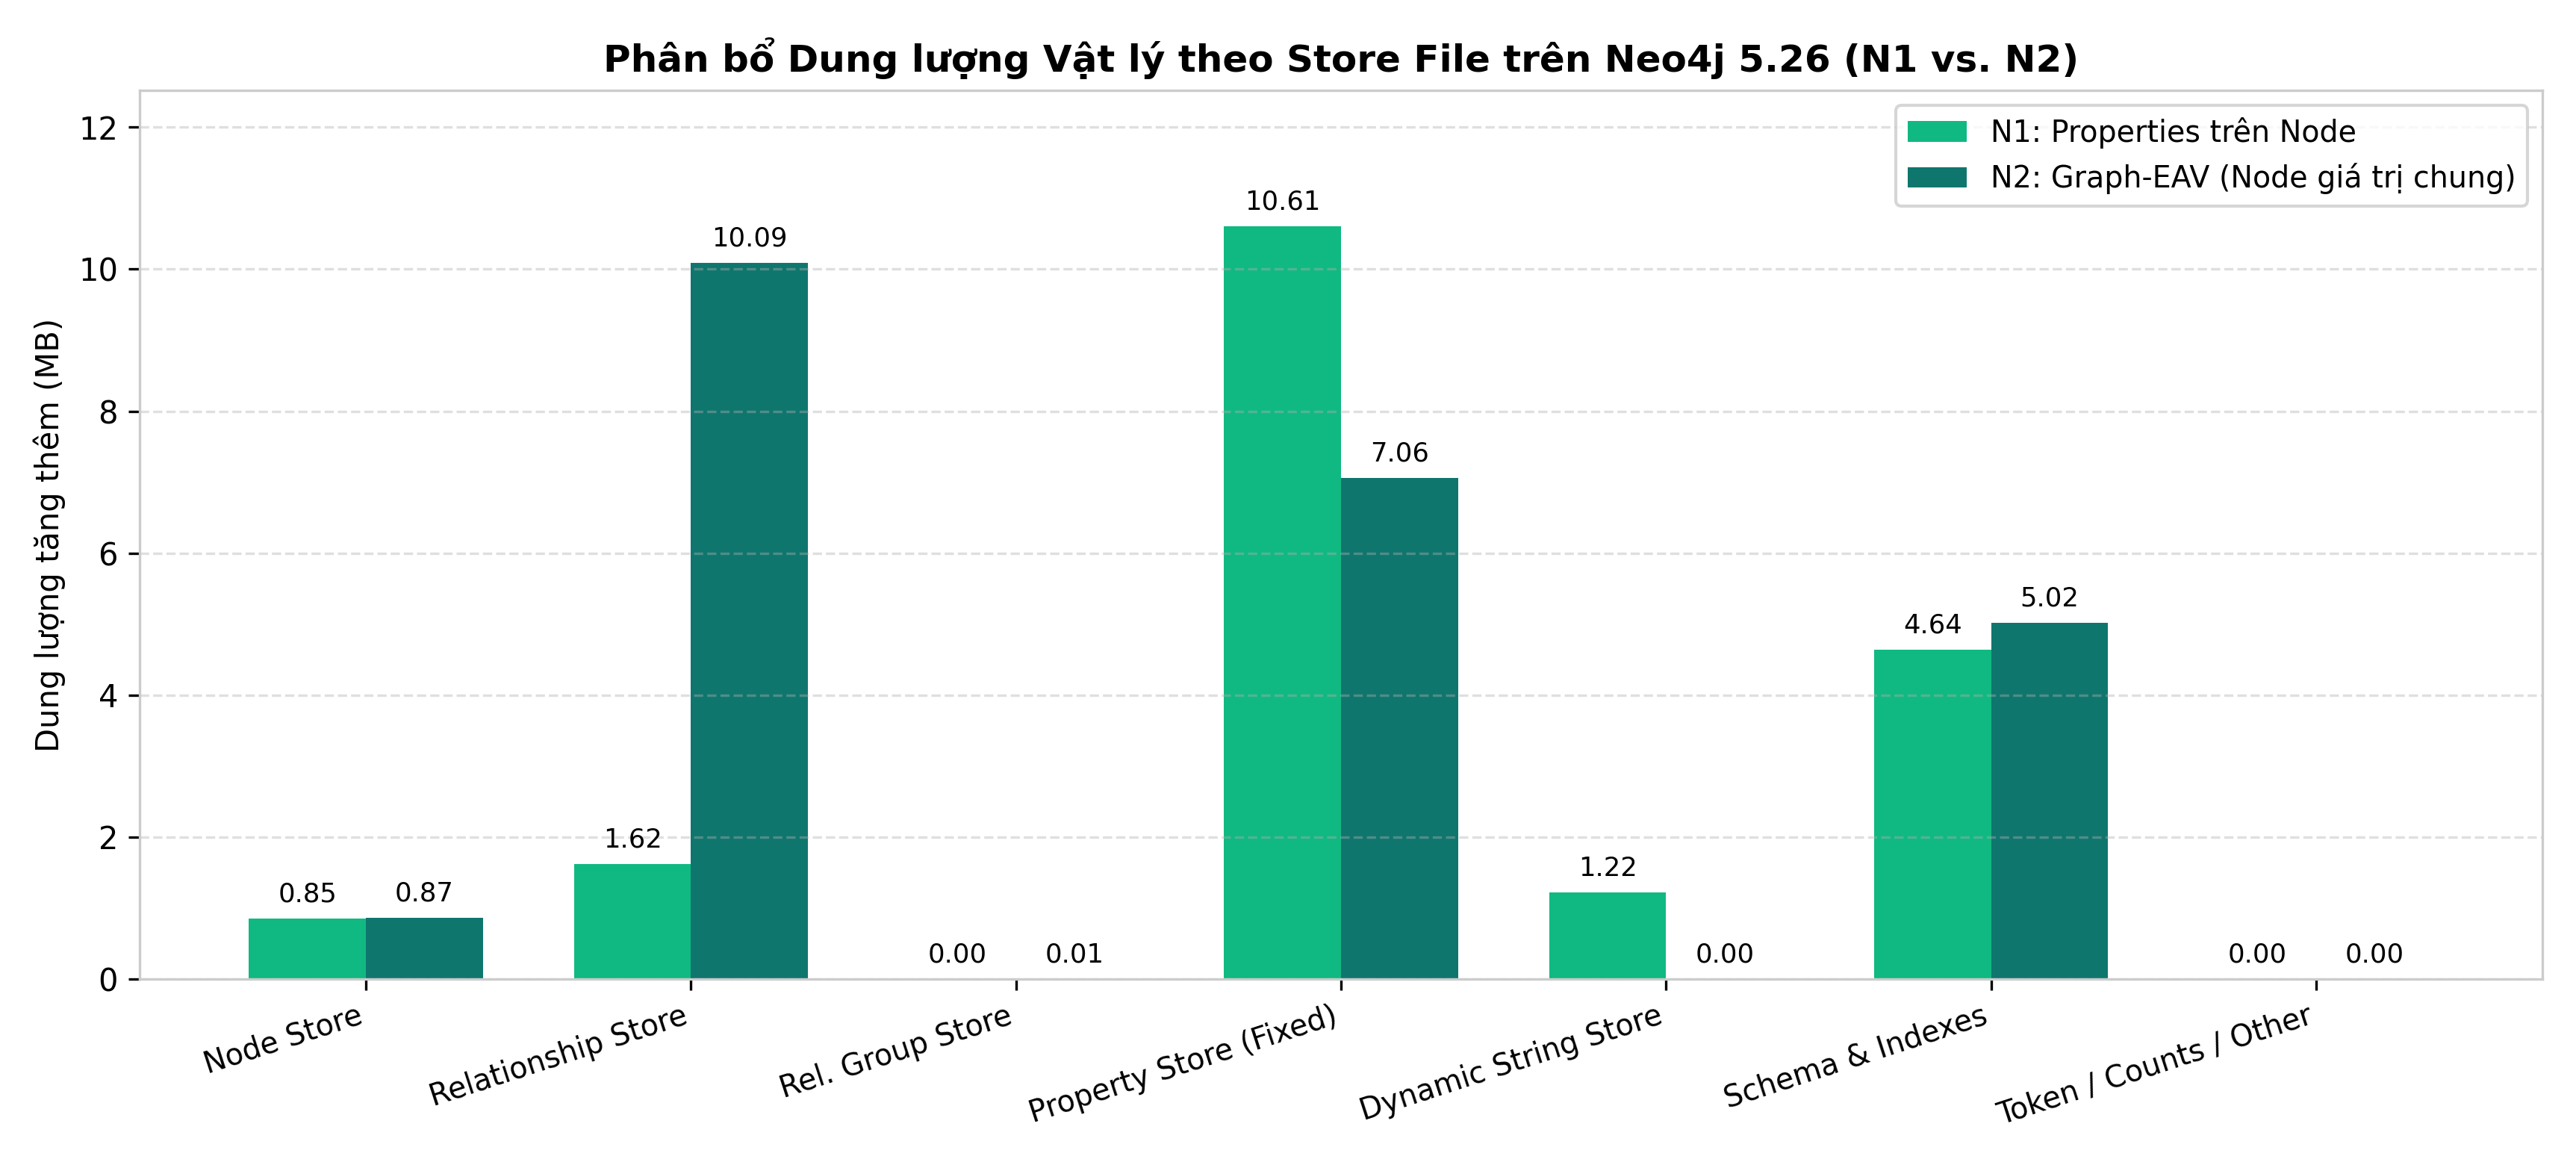
\includegraphics[width=0.95\textwidth]{report/images/topic1_neo4j_store_breakdown.png}
  \caption{Phân bổ dung lượng vật lý theo Store File trên Neo4j 5.26 (N1 vs. N2)}
  \label{fig:t1_neo4j_stores}
\end{figure}

Số liệu đo tại Bảng~\ref{tab:t1_neo4j_stores} và Hình~\ref{fig:t1_neo4j_stores} cho thấy rõ sự dịch chuyển dung lượng giữa các Store File: mô hình \texttt{N1} giữ thuộc tính trên nút làm \texttt{propertystore\_fixed} tăng \textbf{10,61 MB} và \texttt{propertystore\_strings} tăng \textbf{1,22 MB} (do lặp lại 10.000 chuỗi \texttt{isbn\_note}); ngược lại \texttt{N2} (Graph-EAV) triệt tiêu hoàn toàn phần tăng thêm của \texttt{propertystore\_strings} (\textbf{0,00 MB}) nhờ dùng chung nút giá trị, nhưng đẩy mạnh \texttt{relationshipstore} lên \textbf{10,09 MB} để lưu 260.000 cạnh \texttt{[:T1\_HAS\_ATTR]}. Đồng thời, thí nghiệm \textit{Space Reuse} trên 1.000 nút \texttt{:T1DeleteDemo} ghi nhận kích thước tổng trước khi chèn là \textbf{45.457.408 bytes} (\texttt{nodestore = 1.900.544 bytes}), sau khi chèn và checkpoint tăng lên \textbf{46.080.000 bytes} (\texttt{nodestore = 1.916.928 bytes}), và sau khi xóa bằng \texttt{DETACH DELETE} rồi checkpoint lại vẫn giữ mức \textbf{46.096.384 bytes} (\texttt{nodestore = 1.916.928 bytes}), xác nhận tệp vật lý không tự co lại ngay sau khi xóa dữ liệu.

\paragraph{Kịch bản 2: So sánh dung lượng lưu trữ vật lý trên 50.000 biến thể sản phẩm:}
Kịch bản 2 đối chiếu tổng không gian lưu trữ vật lý khi chứa cùng 50.000 biến thể đa ngành hàng giữa 6 mô hình SQL Server (đo từ \texttt{sys.partitions}, \texttt{sys.allocation\_units}, \texttt{sys.dm\_db\_index\_physical\_stats}) và 2 mô hình Neo4j:

\begin{lstlisting}[language=SQL, caption={Trích lược đồ EAV nén PAGE, Native JSON 2025 và SPARSE NULL}, label={lst:t1_sql_models}]
-- M1_EAV_PageComp: EAV value table + covering index with DATA_COMPRESSION = PAGE
CREATE TABLE dbo.T1_Variant_Attr_Values_PageComp (
    variant_id INT NOT NULL, attr_id INT NOT NULL, attr_value NVARCHAR(200) NOT NULL,
    CONSTRAINT PK_T1_EAV_PC PRIMARY KEY CLUSTERED (variant_id, attr_id)
        WITH (DATA_COMPRESSION = PAGE)
);
CREATE NONCLUSTERED INDEX IX_T1_EAV_PC_AttrVal
ON dbo.T1_Variant_Attr_Values_PageComp (attr_id, attr_value)
WITH (DATA_COMPRESSION = PAGE);

-- M2b_JsonNative: Hybrid Relational + Native `json` data type (SQL Server 2025)
CREATE TABLE dbo.T1_Variants_JsonNative (
    variant_id INT NOT NULL PRIMARY KEY CLUSTERED, product_id INT NOT NULL,
    category_name NVARCHAR(30) NOT NULL, sku NVARCHAR(40) NOT NULL,
    price DECIMAL(18,2) NOT NULL, stock_qty INT NOT NULL,
    attributes json NOT NULL
);

-- M3_Sparse: Wide Table with SPARSE NULL columns (0 bytes per NULL value)
CREATE TABLE dbo.T1_Variants_Sparse (
    variant_id INT NOT NULL PRIMARY KEY CLUSTERED, product_id INT NOT NULL,
    category_name NVARCHAR(30) NOT NULL, sku NVARCHAR(40) NOT NULL,
    price DECIMAL(18,2) NOT NULL, stock_qty INT NOT NULL,
    color NVARCHAR(20) NULL, storage_gb INT SPARSE NULL, ram_gb INT SPARSE NULL,
    cpu_model NVARCHAR(40) SPARSE NULL, apparel_size NVARCHAR(10) SPARSE NULL,
    isbn_note NVARCHAR(200) SPARSE NULL -- 20 sparse category columns in total
);
\end{lstlisting}

\begin{table}[htbp]
  \centering
  \scriptsize
  \setlength{\tabcolsep}{3.5pt}
  \renewcommand{\arraystretch}{1.25}
  \setlength{\emergencystretch}{2em}
  \caption{So sánh dung lượng lưu trữ vật lý trên 50.000 biến thể sản phẩm (8 mô hình)}
  \label{tab:t1_storage_50k}
  \begin{tabular}{|p{3.4cm}|p{2.35cm}|p{1.35cm}|p{1.4cm}|p{1.4cm}|p{1.0cm}|p{1.3cm}|}
    \hline
    \textbf{Mô hình lưu trữ} & \textbf{DBMS} & \textbf{Data (MB)} & \textbf{Index (MB)} & \textbf{Total (MB)} & \textbf{B/Var} & \textbf{In-Row Pages} \\
    \hline
    \texttt{M3\_Sparse} (SPARSE)       & SQL Server 2025 & 10,203 &  0,000 & \textbf{10,203} & 214,0 & 1.306 \\ \hline
    \texttt{M1\_EAV\_PageComp}         & SQL Server 2025 &  7,031 &  3,305 & \textbf{10,336} & 216,8 & 1.323 \\ \hline
    \texttt{Control\_WideNoSparse}     & SQL Server 2025 & 10,828 &  0,000 & \textbf{10,828} & 227,1 & 1.386 \\ \hline
    \texttt{M2b\_JsonNative}           & SQL Server 2025 & 14,133 &  0,000 & \textbf{14,133} & 296,4 & 1.809 \\ \hline
    \texttt{M2a\_JsonText}             & SQL Server 2025 & 16,648 &  0,000 & \textbf{16,648} & 349,1 & 2.131 \\ \hline
    \texttt{N1\_Neo4j\_Properties}     & Neo4j 5.26      & 14,305 &  4,641 & \textbf{18,945} & 397,3 & --    \\ \hline
    \texttt{N2\_Neo4j\_GraphEAV}       & Neo4j 5.26      & 18,031 &  5,023 & \textbf{23,055} & 483,5 & --    \\ \hline
    \texttt{M1\_EAV} (Không nén)       & SQL Server 2025 & 13,516 & 11,250 & \textbf{24,766} & 519,4 & 3.170 \\ \hline
  \end{tabular}
\end{table}

\begin{figure}[H]
  \centering
  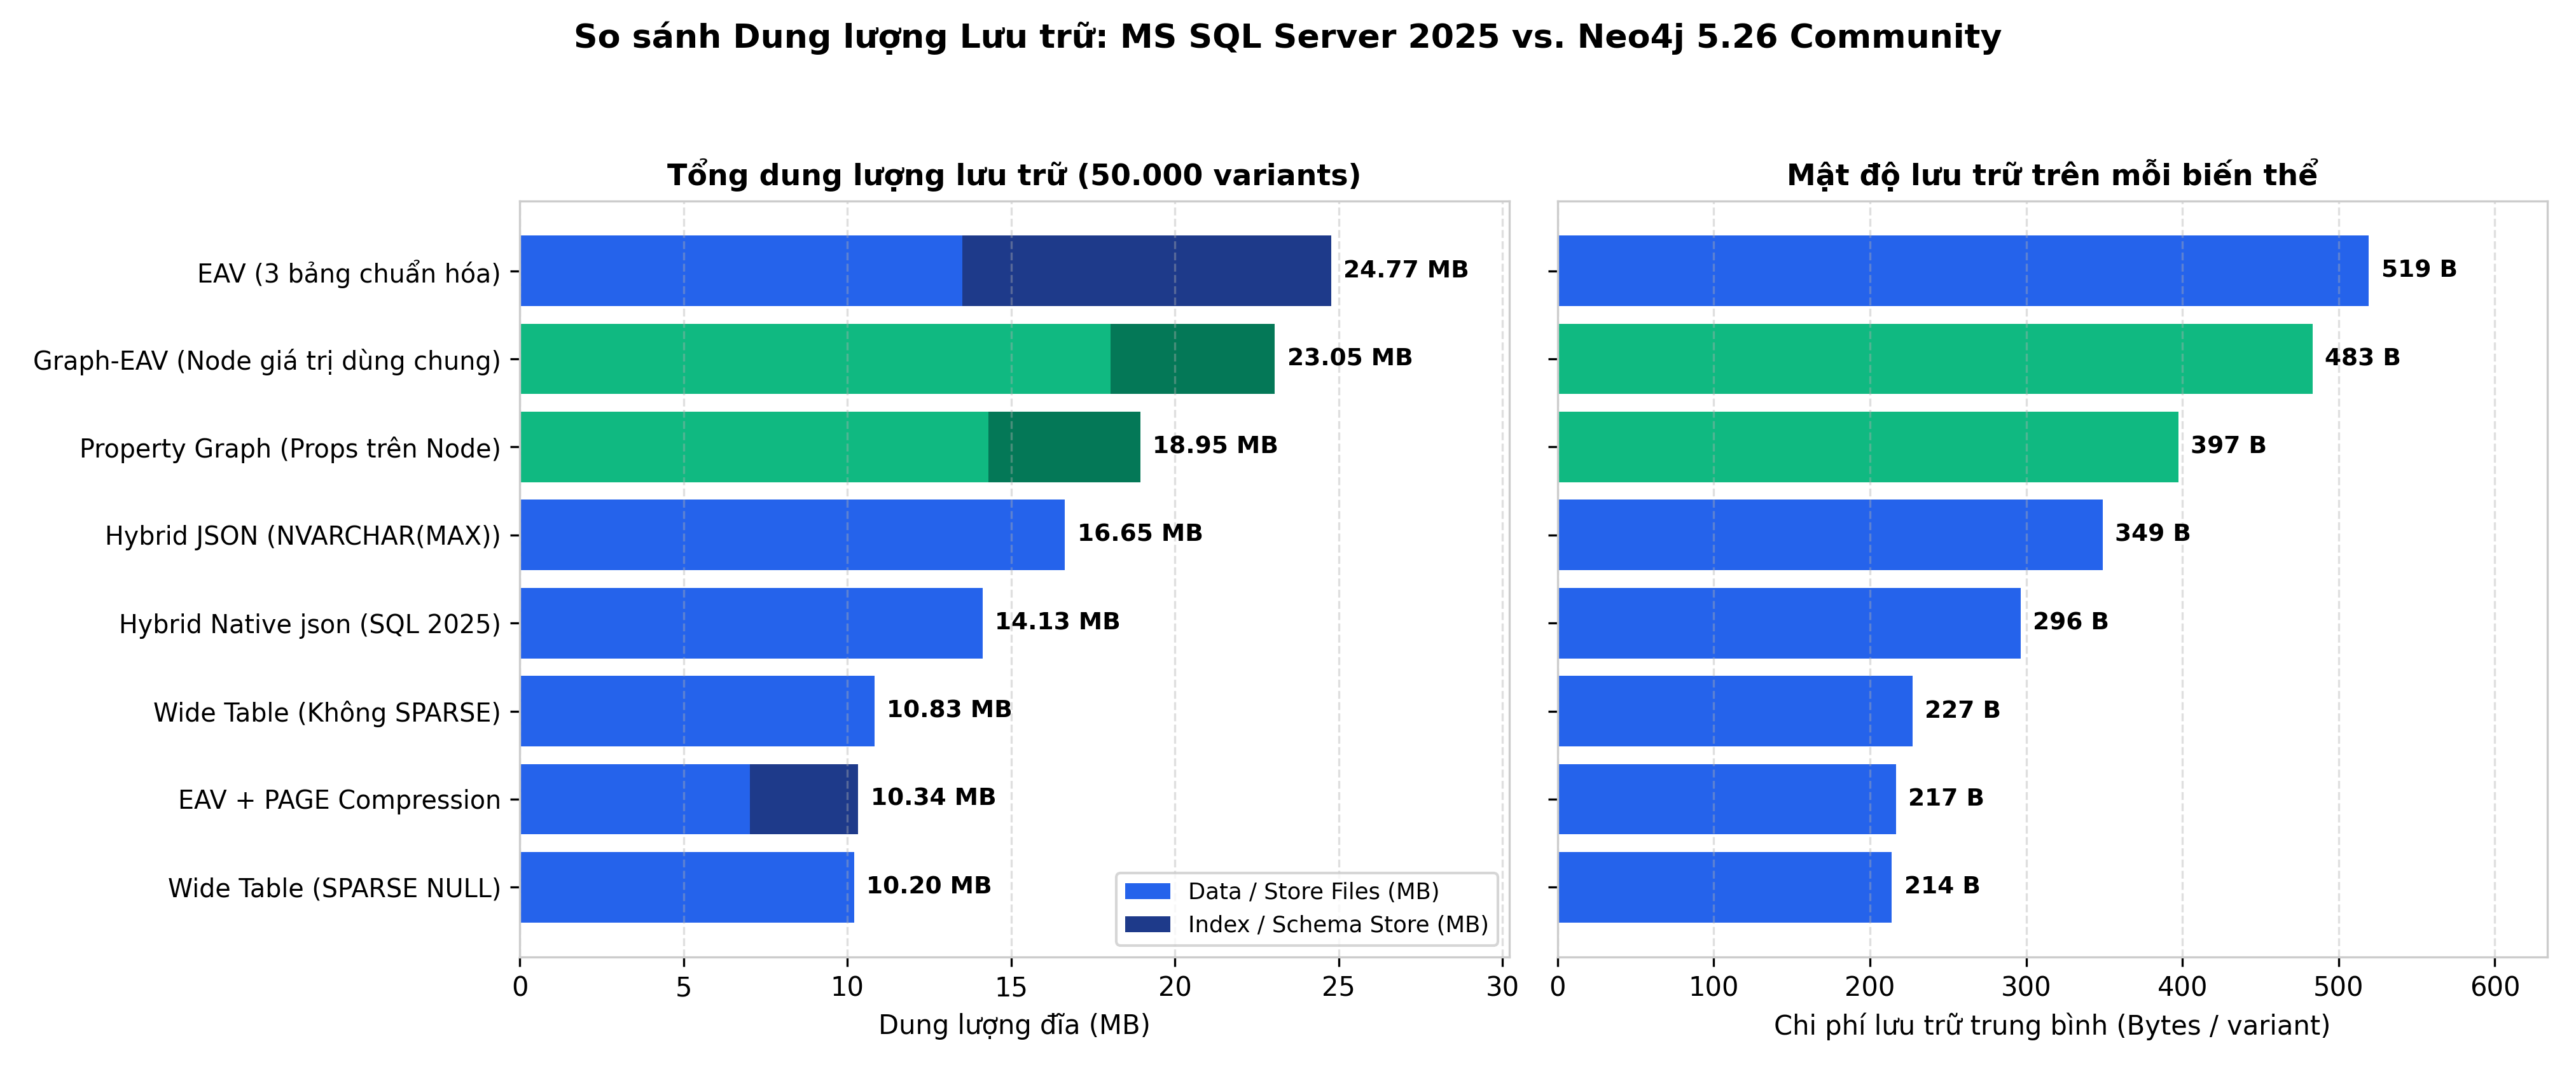
\includegraphics[width=\textwidth]{report/images/topic1_storage_comparison.png}
  \caption{So sánh tổng dung lượng đĩa và mật độ lưu trữ trên mỗi biến thể (50.000 variants)}
  \label{fig:t1_storage_comp}
\end{figure}

Kết quả tại Bảng~\ref{tab:t1_storage_50k} và Hình~\ref{fig:t1_storage_comp} (tất cả bảng SQL đều có 0 trang \texttt{ROW\_OVERFLOW\_DATA} và 0 trang \texttt{LOB\_DATA}) cho thấy bốn điểm nổi bật:
\begin{enumerate}
  \item \textbf{Tác động của nén \texttt{PAGE} lên EAV:} Khi không nén, \texttt{M1\_EAV} tốn nhiều dung lượng nhất (\textbf{24,77 MB}, 519,4 B/biến thể) do nhân thành 260.000 dòng dọc kèm chỉ mục phụ chiếm 11,25 MB. Khi bật \texttt{DATA\_COMPRESSION = PAGE}, nén từ điển và tiền tố nội trang kéo tổng dung lượng giảm \textbf{58,3\%} xuống còn \textbf{10,34 MB} (từ 3.170 xuống 1.323 trang 8 KB).
  \item \textbf{Ưu thế của kiểu \texttt{json} gốc trên SQL Server 2025:} Nhờ lưu nhị phân đã phân tích cú pháp sẵn, \texttt{M2b\_JsonNative} chỉ tiêu tốn \textbf{14,13 MB} (286,37 B/dòng), tiết kiệm trực tiếp \textbf{15,1\%} dung lượng so với \texttt{M2a\_JsonText} lưu văn bản UTF-16 (\textbf{16,65 MB}, 333,79 B/dòng).
  \item \textbf{Hiệu quả thực tế của \texttt{SPARSE NULL}:} Với tỷ lệ \texttt{NULL} 80\% trên 20 cột đặc thù, mô hình \texttt{M3\_Sparse} đạt dung lượng nhỏ nhất (\textbf{10,20 MB}), tiết kiệm \textbf{5,8\%} so với bảng đối chứng \texttt{Control\_WideNoSparse} (\textbf{10,83 MB}) do phần lớn cột chuỗi biến thiên \texttt{NVARCHAR} vốn đã nhỏ gọn khi \texttt{NULL} trong khi cột Sparse phải bù thêm chi phí \textit{Sparse Vector} cho các giá trị khác \texttt{NULL}.
  \item \textbf{Chi phí cấu trúc của Neo4j:} Cả \texttt{N1} (\textbf{18,95 MB}) và \texttt{N2} (\textbf{23,05 MB}) đều lớn hơn các mô hình lai JSON và Sparse của SQL Server vì phải lưu thêm các tệp con trỏ quan hệ hai chiều và chỉ mục nhãn (\texttt{schema\_indexes} chiếm 4,64--5,02 MB).
\end{enumerate}

\paragraph{Kịch bản 3: So sánh khả năng mở rộng Schema (Schema Evolution) và hiệu năng truy vấn (d), (a), (c):}
Kịch bản 3 kiểm tra tốc độ thích ứng khi nghiệp vụ thay đổi và hiệu năng trên nhóm truy vấn thuộc phạm vi Thành viên 1: (1) bổ sung thuộc tính mới \texttt{battery\_mAh = 5000} cho toàn bộ \textbf{10.000 biến thể Smartphones}; (2) chạy \textbf{Truy vấn (d)} điều kiện đơn lọc \texttt{color = 'Black'} (khớp chính xác \textbf{8.000 biến thể} ở cả 8 mô hình, đo trung bình 3 lần sau warmup kèm \texttt{logical reads} / \texttt{PROFILE db hits}); và (3) chạy \textbf{Truy vấn (a)} chèn thuộc tính lạ \texttt{waterproof\_ip = 'IP68'} cùng \textbf{Truy vấn (c)} cập nhật giá và màu cho \texttt{variant\_id = 1}:

\begin{lstlisting}[language=SQL, caption={Thực nghiệm Schema Evolution và truy vấn (d)/(a)/(c) trên MS SQL Server 2025}, label={lst:t1_sql_evo}]
-- 1. Schema Evolution: Wide/Sparse require DDL ALTER TABLE (Sch-M lock)
ALTER TABLE dbo.T1_Variants_Sparse ADD battery_mAh INT SPARSE NULL;
UPDATE dbo.T1_Variants_Sparse
SET battery_mAh = 5000 WHERE category_name = N'Smartphones';

--    Hybrid Native json adds attribute via DML .modify() with ZERO DDL
UPDATE dbo.T1_Variants_JsonNative
SET attributes.modify('$.battery_mAh', 5000)
WHERE category_name = N'Smartphones';

-- 2. Query (d) Single Condition: filter color = 'Black' (8,000 matches)
SELECT COUNT(*) FROM dbo.T1_Variant_Attr_Values_PageComp v
JOIN dbo.T1_Attributes a ON a.attr_id = v.attr_id
WHERE a.attr_name = N'color' AND v.attr_value = N'Black';

SELECT COUNT(*) FROM dbo.T1_Variants_JsonNative
WHERE JSON_VALUE(attributes, '$.color') = N'Black';

-- 3. Query (a) Insert novel attribute & Query (c) Point Update (FR-07)
INSERT INTO dbo.T1_Variants_JsonNative
VALUES (999999, 1, N'Smartphones', N'SKU-DEMO-IP68', 1199.00, 15,
        '{"color":"Black","waterproof_ip":"IP68"}');
UPDATE dbo.T1_Variants_JsonNative
SET price = price + 10.00, attributes.modify('$.color', N'Matte Black')
WHERE variant_id = 1;
\end{lstlisting}

\begin{lstlisting}[language={}, caption={Thực nghiệm Schema Evolution và truy vấn (d)/(a)/(c) trên Neo4j 5}, label={lst:t1_neo_evo}, morekeywords={MATCH,SET,RETURN,count,MERGE,WITH,PROFILE,WHERE,CREATE}, sensitive=false, morecomment={[l]{//}}, morestring={[b]'}]
// 1. Schema Evolution: N1 (SET property, 0 DDL) & N2 (Shared node + 10k edges)
MATCH (v:T1VariantProp {category: 'Smartphones'})
SET v.battery_mAh = 5000 RETURN count(v);

MERGE (a:T1AttrValue {name: 'battery_mAh', value: '5000'})
WITH a MATCH (v:T1VariantGraph {category: 'Smartphones'})
MERGE (v)-[:T1_HAS_ATTR]->(a) RETURN count(v);

// 2. Query (d) Single Condition: LabelScan (N1) vs Index-Free Adjacency (N2)
PROFILE MATCH (v:T1VariantProp) WHERE v.color = 'Black' RETURN count(v);
PROFILE MATCH (:T1AttrValue {name: 'color', value: 'Black'})
              <-[:T1_HAS_ATTR]-(v:T1VariantGraph)
RETURN count(v);

// 3. Query (a) Insert novel property & Query (c) Point Update
MATCH (p:T1Product {product_id: 1})
CREATE (p)-[:T1_HAS_VARIANT]->(:T1VariantProp {
  variant_id: 999999, sku: 'SKU-DEMO-IP68', price: 1199.0,
  color: 'Black', waterproof_ip: 'IP68'
});
MATCH (v:T1VariantProp {variant_id: 1})
SET v.price = v.price + 10.0, v.color = 'Matte Black';
\end{lstlisting}

\begin{table}[htbp]
  \centering
  \scriptsize
  \setlength{\tabcolsep}{3.5pt}
  \renewcommand{\arraystretch}{1.25}
  \setlength{\emergencystretch}{2em}
  \caption{Kết quả thực nghiệm Schema Evolution (10.000 Smartphones) và Truy vấn (d) (8.000 kết quả)}
  \label{tab:t1_evo_query}
  \begin{tabular}{|p{3.3cm}|p{1.2cm}|p{1.1cm}|p{1.9cm}|p{2.4cm}|p{2.1cm}|}
    \hline
    \textbf{Mô hình} & \textbf{Evo (ms)} & \textbf{Qd (ms)} & \textbf{Chi phí đọc} & \textbf{Linh hoạt Schema} & \textbf{An toàn kiểu} \\
    \hline
    \texttt{M1\_EAV}               &   645,12 &          2,03 &     32 \textit{reads} & Cao (Không DDL)         & Yếu (\texttt{NVARCHAR}) \\ \hline
    \texttt{M1\_EAV\_PageComp}     &   737,39 & \textbf{1,06} & \textbf{13 \textit{reads}} & Cao (Không DDL)    & Yếu (\texttt{NVARCHAR}) \\ \hline
    \texttt{M2a\_JsonText}         &   563,72 &        267,00 &  2.887 \textit{reads} & Cao (\texttt{JSON\_\allowbreak MODIFY}) & TB (\texttt{ISJSON}) \\ \hline
    \texttt{M2b\_JsonNative}       &   426,33 &        267,87 &  3.611 \textit{reads} & Cao (\texttt{.modify()}) & TB (Native JSON) \\ \hline
    \texttt{M3\_Sparse}            &   366,21 &         14,84 &  1.904 \textit{reads} & Thấp (DDL \texttt{Sch-M}) & Mạnh (Định kiểu) \\ \hline
    \texttt{Control\_WideNoSparse} &   304,63 &         13,61 &  1.474 \textit{reads} & Thấp (DDL \texttt{Sch-M}) & Mạnh (Định kiểu) \\ \hline
    \texttt{N1\_Neo4j\_Properties} &   758,00 &        123,33 & 100.001 \textit{hits} & Rất cao (0 DDL)         & Yếu (Community) \\ \hline
    \texttt{N2\_Neo4j\_GraphEAV}   & 1.854,00 &         80,33 & 16.004 \textit{hits}  & Rất cao (0 DDL)         & TB (\texttt{AttrValue}) \\ \hline
  \end{tabular}
\end{table}

\begin{figure}[H]
  \centering
  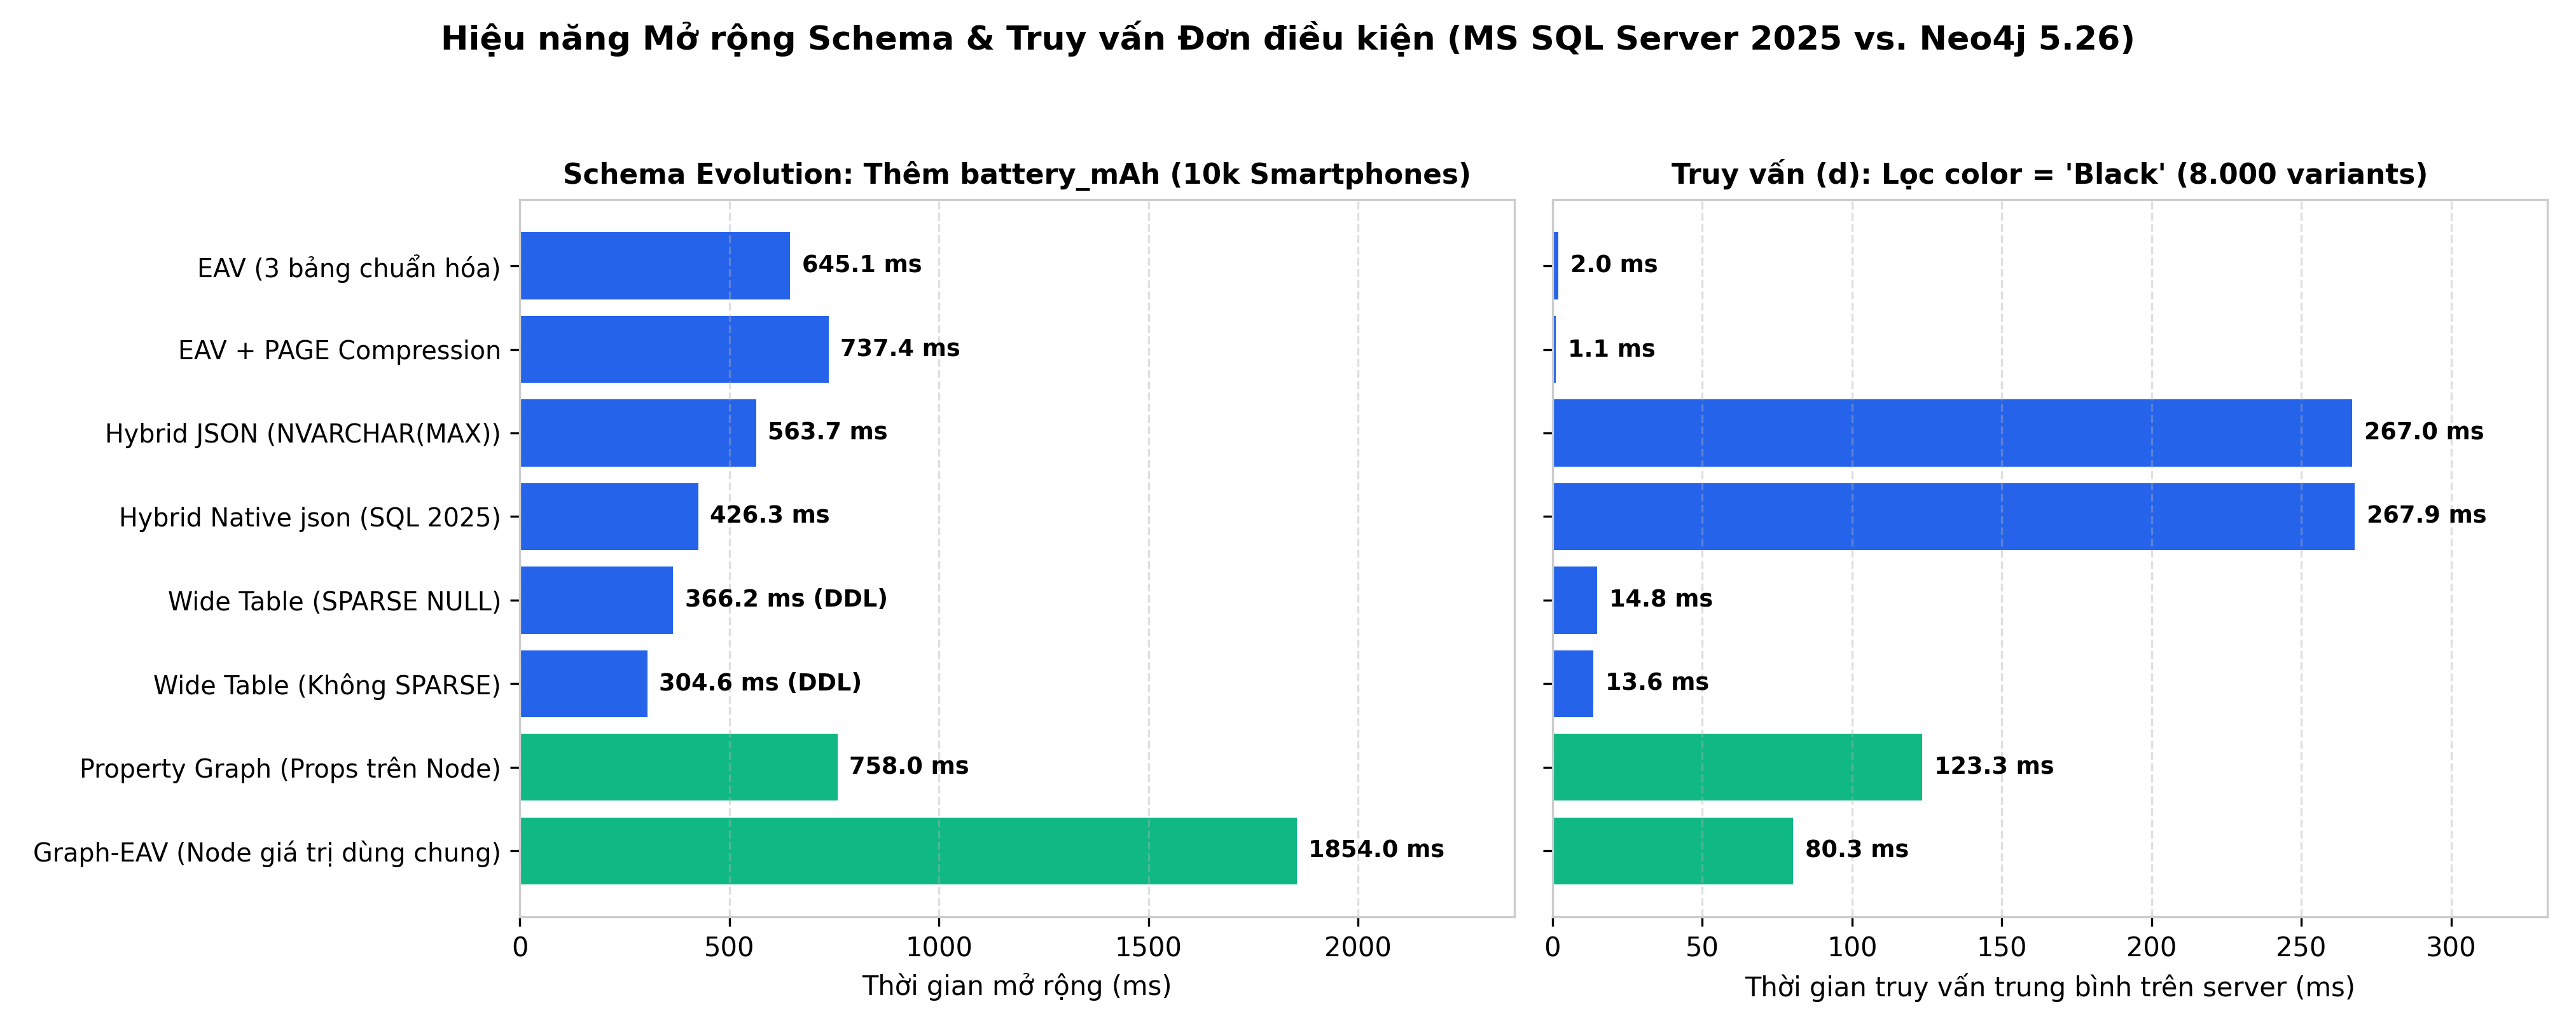
\includegraphics[width=\textwidth]{report/images/topic1_evolution_query.png}
  \caption{Hiệu năng mở rộng Schema và truy vấn đơn điều kiện (MS SQL Server 2025 vs. Neo4j 5.26)}
  \label{fig:t1_evo_query}
\end{figure}

Từ kết quả ở Bảng~\ref{tab:t1_evo_query} và Hình~\ref{fig:t1_evo_query}, có thể phân tích rõ các đánh đổi sau:
\begin{itemize}
  \item \textbf{Mở rộng Schema (\texttt{battery\_mAh}):} Hai bảng rộng \texttt{M3\_Sparse} (366,21 ms) và \texttt{Control\_WideNoSparse} (304,63 ms) phải dùng \texttt{ALTER TABLE} chiếm khóa \textbf{\texttt{Sch-M} (Schema Modification Lock)}, có nguy cơ chặn các giao dịch đồng thời trên hệ thống lớn. Ngược lại, \texttt{M2b\_JsonNative} hoàn tất mở rộng bằng DML \texttt{.modify()} trong \textbf{426,33 ms} (nhanh hơn 24,4\% so với \texttt{JSON\_MODIFY} của \texttt{M2a} ở mức 563,72 ms) mà không cần DDL. Trên Neo4j, \texttt{N1} mở rộng rất gọn bằng \texttt{SET} (758,00 ms), còn \texttt{N2} tốn 1.854,00 ms vì phải tạo mới 10.000 cạnh quan hệ trong \texttt{Relationship Store}.
  \item \textbf{Truy vấn (d) (\texttt{color = 'Black'}):} \texttt{M1\_EAV\_PageComp} đạt tốc độ nhanh nhất (\textbf{1,06 ms}, chỉ \textbf{13 logical reads}) nhờ chỉ mục bao phủ nén \texttt{PAGE}. Hai mô hình JSON chưa tạo chỉ mục computed column phải quét toàn bảng và phân tích JSON nên mất 267,00--267,87 ms. Trên Neo4j, \texttt{N2\_Neo4j\_GraphEAV} (\textbf{80,33 ms}, \textbf{16.004 db hits}) giảm được \textbf{84\% số lần truy cập CSDL} so với \texttt{N1} (\textbf{123,33 ms}, \textbf{100.001 db hits}) do \texttt{N1} phải quét toàn bộ 50.000 nút (\texttt{NodeByLabelScan}), còn \texttt{N2} định vị trực tiếp nút \texttt{:T1AttrValue} và đi theo 8.000 cạnh liền kề bằng \textit{Index-Free Adjacency}.
  \item \textbf{Truy vấn (a) Insert \& (c) Update (FR-07):} Khi thử chèn biến thể mới có thuộc tính lạ \texttt{waterproof\_ip = 'IP68'}, mô hình \texttt{M3\_Sparse} lập tức bị từ chối với lỗi \textbf{Msg 207} (\textit{Invalid column name 'waterproof\_ip'}), thể hiện tính khắt khe của \textit{Schema-on-Write}; trong khi \texttt{M2b\_JsonNative} chèn thành công trong \textbf{5,88 ms} và cập nhật giá + màu cục bộ bằng \texttt{.modify()} chỉ mất \textbf{3,00 ms}. Trên Neo4j, lệnh Cypher đơn lẻ tạo thuộc tính mới kèm dọn dẹp ghi nhận \textbf{669,00 ms} và lệnh cập nhật + khôi phục ghi nhận \textbf{307,00 ms} (do là lượt chạy đơn chưa làm nóng bộ đệm kế hoạch thực thi và bao gồm thao tác dọn dẹp trong cùng phiên \texttt{cypher-shell}).
\end{itemize}

\subsubsection{Đánh giá và quyết định}

Bảng~\ref{tab:t1_summary} tổng hợp các đặc tính cốt lõi về lưu trữ và quản trị dữ liệu giữa MS SQL Server 2025 và Neo4j 5.26:

\begin{table}[htbp]
  \centering
  \footnotesize
  \setlength{\tabcolsep}{4pt}
  \renewcommand{\arraystretch}{1.25}
  \setlength{\emergencystretch}{2em}
  \caption{So sánh tổng hợp cơ chế Data Storage \& Management giữa MS SQL Server và Neo4j}
  \label{tab:t1_summary}
  \begin{tabular}{|p{2.9cm}|p{5.0cm}|p{5.0cm}|}
    \hline
    \textbf{Tiêu chí} & \textbf{MS SQL Server (2025)} & \textbf{Neo4j (5.26 LTS)} \\
    \hline
    Mô hình dữ liệu & Relational Model & Labeled Property Graph \\ \hline
    Thiết kế Schema & Schema-on-Write (ép ràng buộc khi ghi) & Schema-Optional (linh hoạt thuộc tính) \\ \hline
    Tổ chức dữ liệu & Tables, Rows, Columns & Nodes, Relationships, Properties \\ \hline
    Đơn vị lưu trữ & Page 8 KB, Extent 64 KB & Record Store (Aligned) hoặc Block Store \\ \hline
    Cấu trúc lưu trữ & Heap, Clustered Index B+Tree & Node, Relationship, Property Store \\ \hline
    Truy xuất quan hệ & Foreign Key và JOIN & Index-Free Adjacency ($O(1)$/bước nhảy) \\ \hline
    Dữ liệu lớn / động & Row Overflow, LOB, Native \texttt{json}, Sparse & Inline Storage và Dynamic Storage \\ \hline
    Bộ nhớ đệm & Buffer Pool & Off-Heap Page Cache (tách JVM Heap) \\ \hline
    Cơ chế nén & Row Compression, Page Compression & Phụ thuộc Store Format \\ \hline
    Mở rộng thuộc tính & \texttt{ALTER TABLE} (\texttt{Sch-M}) hoặc EAV/JSON & \texttt{SET}/\texttt{CREATE} tức thì (0 DDL) \\ \hline
    Phục hồi dữ liệu & Transaction Log, Checkpoint, REDO/UNDO & Transaction Log, Checkpoint, Recovery \\ \hline
    Thu hồi không gian & Ghost Cleanup, REBUILD, REORGANIZE & Space Reuse và Defragmentation \\ \hline
  \end{tabular}
\end{table}

\paragraph{Quyết định lựa chọn cho hệ thống E-Commerce:} Từ phân tích lý thuyết và số liệu thực nghiệm trên, nhóm quyết định chọn \textbf{MS SQL Server} làm hệ quản trị cơ sở dữ liệu chính cho nền tảng thương mại điện tử đa gian hàng vì ba lý do then chốt:

\begin{enumerate}
  \item \textbf{Bảo toàn tính toàn vẹn bằng Schema-on-Write:} Hệ thống E-Commerce xoay quanh các thực thể giao dịch tài chính và tồn kho (\texttt{Users}, \texttt{Sellers}, \texttt{Products}, \texttt{Orders}, \texttt{Order\_Details}, \texttt{Vouchers}), đòi hỏi cơ chế kiểm tra kiểu dữ liệu, khóa ngoại và ràng buộc \texttt{CHECK} nghiêm ngặt ngay tại tầng Storage Engine (như đã chứng minh bằng lỗi 547 khi chặn giá âm).
  \item \textbf{Hiệu quả nén và lưu trữ đa dạng trên trang 8 KB:} Kiến trúc Page 8 KB kết hợp \texttt{DATA\_COMPRESSION = PAGE} (216,8 B/biến thể) và mô hình lai Native \texttt{json} (296,4 B/biến thể, 0 DDL khi mở rộng) giúp tối ưu dung lượng đĩa vượt trội so với Neo4j (397,3--483,5 B/biến thể), vừa giữ trọn lợi thế quan hệ vừa linh hoạt cho biến thể sản phẩm.
  \item \textbf{Khả năng kết hợp Polyglot Persistence trong tương lai:} Neo4j không phù hợp thay thế cho CSDL giao dịch chính do thiếu chuẩn hóa ràng buộc bảng, nhưng rất lý tưởng để vận hành song song cho các phân hệ phân tích đồ thị nhiều tầng như hệ thống gợi ý sản phẩm cá nhân hóa hoặc phát hiện gian lận liên kết giữa \texttt{Users} -- \texttt{Orders} -- \texttt{Sellers}.
\end{enumerate}


% ==============================================================================
% CÁC ĐOẠN CẦN BỔ SUNG VÀO CÁC VỊ TRÍ KHÁC TRONG main.tex (BỎ COMMENT KHI DÁN)
% ==============================================================================
%
% --- [1] Dòng bổ sung vào Bảng 1 (Danh sách thành viên & Phân công công việc) ---
% 2 & Trần Quốc Hiền & 2310992 &
%   - Nghiên cứu chủ đề Data Storage \& Schema Design (MS SQL Server vs Neo4j) \newline
%   - Thiết kế lược đồ ECommerceDB và hiện thực FR-02, FR-07, AuthModule & 100\% \\ \hline
%
% --- [2] Sửa lỗi tiêu đề "Tài liệu" bị cắt chữ ở cuối main.tex (nếu dùng babel vietnamese) ---
% Thêm dòng này trước \begin{document} trong main.tex:
% \addto\captionsvietnamese{\renewcommand{\refname}{Tài liệu tham khảo}}
%
% --- [3] 9 Tài liệu tham khảo nối tiếp sau [10] trong \begin{thebibliography} ---
% \bibitem{t1_date2004}
% C.~J. Date, \textit{An Introduction to Database Systems}, 8th~ed. Pearson, 2004.
%
% \bibitem{t1_silberschatz2019}
% A.~Silberschatz, H.~F. Korth, and S.~Sudarshan, \textit{Database System Concepts}, 7th~ed. McGraw-Hill, 2019.
%
% \bibitem{t1_delaney2012}
% K.~Delaney et~al., \textit{Microsoft SQL Server 2012 Internals}. Microsoft Press, 2012.
%
% \bibitem{t1_mspages}
% Microsoft Learn, \textit{Pages and Extents Architecture Guide -- SQL Server}. [Online]. Available: \url{https://learn.microsoft.com/en-us/sql/relational-databases/pages-and-extents-architecture-guide}
%
% \bibitem{t1_mssparse}
% Microsoft Learn, \textit{Use Sparse Columns -- SQL Server}. [Online]. Available: \url{https://learn.microsoft.com/en-us/sql/relational-databases/tables/use-sparse-columns}
%
% \bibitem{t1_mscomp}
% Microsoft Learn, \textit{Data Compression -- SQL Server}. [Online]. Available: \url{https://learn.microsoft.com/en-us/sql/relational-databases/data-compression/data-compression}
%
% \bibitem{t1_msnativejson}
% Microsoft Learn, \textit{JSON data type (SQL Server 2025)}. [Online]. Available: \url{https://learn.microsoft.com/en-us/sql/t-sql/data-types/json-data-type}
%
% \bibitem{t1_robinson2015}
% I.~Robinson, J.~Webber, and E.~Eifrem, \textit{Graph Databases: New Opportunities for Connected Data}, 2nd~ed. O'Reilly Media, 2015.
%
% \bibitem{t1_neo4jops}
% Neo4j Documentation, \textit{Operations Manual: Store Formats, Memory Configuration, Transaction Logs and Checkpointing}. [Online]. Available: \url{https://neo4j.com/docs/operations-manual/current/}

%      (hoặc copy-paste toàn bộ nội dung từ \subsubsection{...} đến trước phần
%      comment ở cuối file này).
%   3. Cập nhật Bảng 1 (Danh sách thành viên) và nối các \bibitem{t1_...} ở cuối
%      file này vào khối \begin{thebibliography} của main.tex.
% ==============================================================================

\subsubsection{Khái niệm chung về Data Storage và Data Management}

\textbf{Data Storage (Lưu trữ dữ liệu)} là quá trình tổ chức, cấu trúc hóa và duy trì dữ liệu dưới các định dạng nhị phân phù hợp trên thiết bị lưu trữ thứ cấp (SSD/HDD) nhằm bảo đảm độ bền lâu dài, hiệu quả truy xuất và khả năng mở rộng khi khối lượng dữ liệu gia tăng. Thành phần đảm nhiệm trực tiếp chức năng này bên trong một hệ quản trị cơ sở dữ liệu (DBMS) là \textbf{Storage Engine} -- lớp phần mềm cốt lõi chịu trách nhiệm cấp phát không gian đĩa, quản lý bộ nhớ đệm (\textit{Buffer Pool} hoặc \textit{Page Cache}) và duy trì nhật ký giao dịch (\textit{Transaction Log}) phục vụ khôi phục dữ liệu~\cite{t1_date2004,t1_silberschatz2019}.

\textbf{Data Management (Quản trị dữ liệu)} bao gồm tập hợp các cơ chế vận hành trên dữ liệu đã lưu trữ: kiểm soát toàn vẹn ngữ nghĩa và ràng buộc tham chiếu, thực thi truy vấn, xử lý giao dịch (\textit{Transaction}), điều khiển đồng thời, thu hồi không gian trống và bảo đảm tính bền vững sau sự cố. Kiến trúc lưu trữ ở tầng vật lý ảnh hưởng trực tiếp đến chi phí I/O, hiện tượng phân mảnh trang đĩa, dung lượng lưu trữ tiêu thụ cũng như mức độ linh hoạt khi nghiệp vụ thay đổi.

Trong bài toán thực tế của nhóm là nền tảng sàn thương mại điện tử đa gian hàng (\textit{Multi-Vendor E-Commerce Platform}, CSDL \texttt{ECommerceDB}), hệ thống vừa đòi hỏi tính nhất quán chặt chẽ ở các bảng giao dịch cốt lõi (\texttt{Users}, \texttt{Sellers}, \texttt{Orders}, \texttt{Order\_Details}, \texttt{Vouchers}), vừa phát sinh bài toán đặc trưng về \textbf{thuộc tính biến thể sản phẩm linh hoạt}: sản phẩm thuộc ngành hàng \textit{Smartphones} cần lưu \texttt{storage\_gb}, \texttt{ram\_gb}, \texttt{screen\_inch}, \texttt{chipset}; ngành hàng \textit{Laptops} cần \texttt{cpu\_model}, \texttt{gpu\_model}, \texttt{os\_name}; ngành hàng \textit{Fashion} cần \texttt{apparel\_size}, \texttt{material}, \texttt{fit\_style}; còn ngành hàng \textit{Books} lại cần \texttt{author\_name}, \texttt{publisher}, \texttt{page\_count} và \texttt{isbn\_note}. Cách tiếp cận bài toán này phản ánh rõ sự đối lập giữa hai triết lý thiết kế dữ liệu:

\begin{itemize}
  \item \textbf{MS SQL Server (Schema-on-Write):} Yêu cầu khai báo tường minh toàn bộ cấu trúc bảng, kiểu dữ liệu và các ràng buộc (\texttt{PRIMARY KEY}, \texttt{FOREIGN KEY}, \texttt{CHECK}, \texttt{NOT NULL}, \texttt{UNIQUE}) trước khi ghi dữ liệu. Mọi thao tác \texttt{INSERT} hoặc \texttt{UPDATE} đều được kiểm tra nghiêm ngặt ngay tại thời điểm ghi nhằm bảo đảm tính nhất quán cao.
  \item \textbf{Neo4j (Schema-Optional):} Lưu trữ theo mô hình đồ thị thuộc tính có nhãn (\textit{Labeled Property Graph}), cho phép các nút cùng nhãn mang tập thuộc tính khác nhau và bổ sung thuộc tính mới ngay trong quá trình ghi mà không cần chỉnh sửa lược đồ tĩnh, đồng thời vẫn hỗ trợ \textit{Indexes} và \textit{Constraints} để kiểm soát các khóa định danh quan trọng~\cite{t1_robinson2015,t1_neo4jops}.
\end{itemize}

\subsubsection{Đặc trưng cơ chế Data Storage và Data Management trong MS SQL Server}

\paragraph{Mô hình tổ chức và thiết kế dữ liệu cho thuộc tính động:}
MS SQL Server tổ chức dữ liệu logic dưới dạng bảng hai chiều (\textit{Tables, Rows, Columns}) và cung cấp hai cấu trúc lưu trữ vật lý nền tảng cho dữ liệu hàng (\textit{Rowstore})~\cite{t1_delaney2012,t1_mspages}:
\begin{itemize}
  \item \textbf{Heap:} Bảng không có \textit{Clustered Index}; các dòng dữ liệu được lưu tự do không theo thứ tự khóa và được định vị thông qua địa chỉ vật lý \textbf{RID} (\textit{FileID:PageID:SlotID}).
  \item \textbf{Clustered Index:} Tổ chức bảng dưới dạng cây cân bằng \textbf{B+Tree}, trong đó các nút lá chứa trực tiếp toàn bộ dữ liệu dòng được sắp xếp theo thứ tự khóa cụm (mặc định gắn với \texttt{PRIMARY KEY}).
\end{itemize}

Khi mô hình hóa tập thuộc tính biến thể đa dạng trên nền tảng chuẩn hóa quan hệ (1NF--3NF), các hệ thống dùng SQL Server thường áp dụng một trong ba hướng thiết kế sau:
\begin{itemize}
  \item \textbf{Mô hình Entity--Attribute--Value (EAV):} Tách danh mục thuộc tính sang bảng \texttt{Attributes} và lưu từng cặp thuộc tính--giá trị dưới dạng các dòng dọc trong bảng \texttt{Variant\_Attr\_Values}. EAV cho phép thêm thuộc tính mới bằng lệnh \texttt{INSERT} (không cần DDL), nhưng làm tăng mạnh số dòng dữ liệu, giảm an toàn kiểu dữ liệu (thường phải lưu chuỗi \texttt{NVARCHAR}) và phát sinh nhiều phép \texttt{JOIN} khi truy xuất nhiều thuộc tính cùng lúc.
  \item \textbf{Wide Table với Sparse Columns:} Khai báo tất cả thuộc tính của mọi ngành hàng thành các cột trên một bảng rộng kèm từ khóa \texttt{SPARSE NULL}~\cite{t1_mssparse}. Mỗi giá trị \texttt{NULL} trên cột Sparse tiêu thụ \textbf{0 byte} lưu trữ, nhưng mỗi giá trị khác \texttt{NULL} phát sinh thêm 2--4 byte chi phí quản lý trong cấu trúc \textit{Sparse Vector} (chỉ đạt hiệu quả nén khi tỷ lệ \texttt{NULL} cao, thường $\ge$ 20--40\% tùy kiểu dữ liệu) và vẫn phụ thuộc vào lệnh DDL \texttt{ALTER TABLE} khi cần thêm cột mới.
  \item \textbf{Mô hình Hybrid JSON (\texttt{NVARCHAR(MAX)} và kiểu \texttt{json} gốc trên SQL Server 2025):} Giữ các cột giao dịch cốt lõi (\texttt{variant\_id}, \texttt{product\_id}, \texttt{sku}, \texttt{price}, \texttt{stock\_qty}) dưới dạng quan hệ chuẩn định kiểu chặt chẽ, còn tập thuộc tính đặc thù theo ngành hàng được đóng gói vào cột bán cấu trúc. Trước đây, dữ liệu JSON được lưu dưới dạng chuỗi UTF-16 trong \texttt{NVARCHAR(MAX)} kèm ràng buộc \texttt{CHECK} \texttt{(ISJSON(col) = 1)} và cập nhật qua \texttt{JSON\_MODIFY()}. Từ phiên bản \textbf{MS SQL Server 2025}, hệ thống bổ sung kiểu dữ liệu \textbf{\texttt{json} gốc (Native \texttt{json} Data Type)} lưu ở định dạng nhị phân đã phân tích cú pháp sẵn (\textit{pre-parsed binary}) cùng phương thức \texttt{.modify()} trực tiếp, giúp tiết kiệm dung lượng đĩa và giảm chi phí phân tích cú pháp~\cite{t1_msnativejson}.
\end{itemize}

\paragraph{Kiến trúc tệp và trang lưu trữ (Page \& Extent):}
Ở tầng vật lý, mỗi CSDL SQL Server sử dụng ba loại tệp chính: \texttt{.mdf} (tệp dữ liệu chính), \texttt{.ndf} (tệp dữ liệu phụ) và \texttt{.ldf} (tệp nhật ký giao dịch)~\cite{t1_mspages}. Không gian bên trong tệp dữ liệu được chia nhỏ thành các đơn vị lưu trữ chuẩn hóa~\cite{t1_delaney2012,t1_mspages}:
\begin{itemize}
  \item \textbf{Page:} Đơn vị I/O cơ bản có kích thước cố định \textbf{8 KB (8.192 bytes)}, gồm ba vùng chính: (1) \textit{Page Header} (96 bytes đầu chứa mã trang \texttt{m\_pageId}, loại trang \texttt{m\_type}, số dòng \texttt{m\_slotCnt}, vùng trống \texttt{m\_freeCnt}, số bản ghi ma \texttt{m\_ghostRecCnt} và LSN gần nhất \texttt{m\_lsn}); (2) \textit{Data Area} (nơi lưu nối tiếp các dòng dữ liệu); và (3) \textit{Slot Array} ở cuối trang lưu offset trỏ về vị trí từng dòng theo thứ tự logic.
  \item \textbf{Extent:} Gồm \textbf{8 Page liên tiếp}, tương đương \textbf{64 KB}, gồm \textit{Uniform Extent} (cấp phát cho một đối tượng duy nhất) và \textit{Mixed Extent} (chia sẻ giữa tối đa 8 đối tượng nhỏ).
\end{itemize}

\paragraph{Lưu trữ dữ liệu lớn (Allocation Units) và cơ chế nén:}
SQL Server quản lý dữ liệu có kích thước thay đổi thông qua ba \textbf{Allocation Units}~\cite{t1_mspages}:
\begin{itemize}
  \item \textbf{\texttt{IN\_ROW\_DATA}:} Lưu các cột cố định và biến thiên trực tiếp trên trang dữ liệu chính với giới hạn dòng chuẩn tối đa \textbf{8.060 bytes}.
  \item \textbf{\texttt{ROW\_OVERFLOW\_DATA}:} Tự động đẩy các cột độ dài biến thiên (như \texttt{VARCHAR}, \texttt{NVARCHAR}) sang trang tràn dòng khi tổng kích thước dòng vượt quá 8.060 bytes, giữ lại con trỏ 24-byte trên trang gốc.
  \item \textbf{\texttt{LOB\_DATA}:} Lưu trữ các kiểu dữ liệu khối lớn như \texttt{VARCHAR(MAX)}, \texttt{NVARCHAR(MAX)}, \texttt{VARBINARY\allowbreak(MAX)} hoặc \texttt{json} vượt ngưỡng lưu nội dòng.
\end{itemize}

Để tối ưu dung lượng đĩa và I/O bộ nhớ đệm, SQL Server hỗ trợ hai cơ chế nén tích hợp (\texttt{DATA\_COMPRESSION})~\cite{t1_mscomp}: \textbf{Row Compression} chuyển kiểu dữ liệu cố định sang biểu diễn độ dài biến thiên theo giá trị thực và loại bỏ byte đệm trống; trong khi \textbf{Page Compression} kết hợp tuần tự \textit{Row Compression}, \textit{Prefix Compression} (trích xuất tiền tố chung của cột) và \textit{Dictionary Compression} (thay thế giá trị lặp lại toàn trang bằng từ điển nội trang).

\paragraph{Quản lý không gian, phân mảnh và Transaction Log:}
SQL Server theo dõi không gian cấp phát qua các trang bitmap chuyên biệt gồm \textbf{GAM/SGAM} (trạng thái cấp phát Extent), \textbf{PFS} (tỷ lệ chỗ trống của từng Page) và \textbf{IAM} (ánh xạ các Extent thuộc một Allocation Unit)~\cite{t1_mspages}. Khi thêm, sửa hoặc xóa dữ liệu liên tục, hệ thống có thể phát sinh \textbf{Page Split} (tách đôi trang lá B+Tree đã đầy khi chèn khóa mới), \textbf{Forwarded Record} (dòng trên bảng Heap phình to phải dời sang trang khác để lại con trỏ chuyển tiếp), và \textbf{Ghost Record} (đánh dấu logic bản ghi bị xóa hoặc hủy bỏ trên trang lá để tiến trình nền \textit{Ghost Cleanup} thu hồi sau). Quản trị viên bảo trì cấu trúc bằng \texttt{REORGANIZE}/\texttt{REBUILD} và thu hồi dung lượng tệp đĩa bằng \texttt{DBCC SHRINKFILE}. Toàn bộ biến động trên \textit{Buffer Pool} tuân thủ nguyên tắc \textbf{Write-Ahead Logging (WAL)}, kết hợp tiến trình \textbf{Checkpoint} và cơ chế \textbf{REDO/UNDO} từ Transaction Log để đảm bảo phục hồi bền vững~\cite{t1_delaney2012}.

\subsubsection{Đặc trưng cơ chế Data Storage và Data Management trong Neo4j}

\paragraph{Mô hình Labeled Property Graph:}
Neo4j lưu trữ dữ liệu trực tiếp theo mô hình \textbf{Labeled Property Graph (LPG)} gồm ba thành phần cốt lõi~\cite{t1_robinson2015,t1_neo4jops}:
\begin{itemize}
  \item \textbf{Nodes (Nút):} Đại diện cho thực thể (ví dụ \texttt{:User}, \texttt{:Product}, \texttt{:T1VariantProp}); mỗi nút có thể mang một hoặc nhiều nhãn (\textit{Labels}).
  \item \textbf{Relationships (Quan hệ):} Biểu diễn liên kết có hướng và có kiểu giữa nút nguồn và nút đích, ví dụ \texttt{(User)-[:PLACED]->(Order)} hay \texttt{(Product)-\allowbreak[:HAS\_VARIANT]->\allowbreak(Variant)}; mỗi cạnh cũng có thể mang thuộc tính riêng.
  \item \textbf{Properties (Thuộc tính):} Các cặp \textit{Key--Value} linh hoạt gắn trực tiếp lên Node hoặc Relationship.
\end{itemize}

\paragraph{Native Graph Storage và Index-Free Adjacency:}
Neo4j tổ chức dữ liệu đồ thị gốc thành các tệp store vật lý chuyên biệt có kích thước bản ghi cố định trong thư mục dữ liệu~\cite{t1_neo4jops}:
\begin{itemize}
  \item \textbf{Node Store (\texttt{neostore.nodestore.db}):} Lưu thông tin nút, nhãn và con trỏ trỏ tới quan hệ đầu tiên cùng chuỗi thuộc tính đầu tiên.
  \item \textbf{Relationship Store (\texttt{neostore.relationshipstore.db}):} Lưu nút nguồn, nút đích, loại quan hệ và chuỗi liên kết đôi đến các quan hệ kế tiếp của hai đầu nút.
  \item \textbf{Relationship Group Store (\texttt{neostore.\allowbreak relationshipgroupstore.db}):} Gom nhóm cạnh theo loại và chiều đối với các \textit{dense nodes} (nút có mật độ kết nối lớn).
  \item \textbf{Property Store (\texttt{neostore.propertystore.db}) \& Dynamic Store:} Lưu bản ghi thuộc tính cố định và tham chiếu đến vùng lưu trữ động.
\end{itemize}

Neo4j hỗ trợ nhiều \textbf{Store Format} khác nhau theo phiên bản và ấn bản: \textit{Aligned Format} là định dạng mặc định trên ấn bản Community Edition (tối ưu sắp thẳng biên trang với kích thước bản ghi nhẹ), trong khi \textit{Block Format} được sử dụng mặc định trên các phiên bản Enterprise Edition tương ứng~\cite{t1_neo4jops}. Nhờ lưu trực tiếp con trỏ cạnh ngay tại mỗi nút, Neo4j đạt được cơ chế \textbf{Index-Free Adjacency}: hệ thống duyệt qua các mối liên kết lân cận theo tham chiếu trực tiếp với chi phí $O(1)$ cho mỗi bước nhảy mà không cần tra cứu chỉ mục toàn cục như phép \texttt{JOIN} trong SQL Server~\cite{t1_robinson2015}. Tuy nhiên, nếu truy vấn lọc thuộc tính trên toàn bộ nút mà không qua cạnh hoặc chỉ mục, Neo4j vẫn phải quét nhãn (\texttt{NodeByLabelScan}).

\paragraph{Lưu trữ thuộc tính động, Page Cache và Transaction Log:}
Để cân bằng tốc độ truy cập và kích thước thuộc tính biến thiên, Neo4j kết hợp hai cơ chế lưu thuộc tính~\cite{t1_neo4jops}:
\begin{itemize}
  \item \textbf{Inline Storage:} Các giá trị nguyên thủy và chuỗi ngắn vừa kích thước khối thuộc tính được mã hóa và lưu trực tiếp trong \texttt{Property Store}, hạn chế đọc thêm tệp ngoài.
  \item \textbf{Dynamic Storage:} Các chuỗi dài hoặc mảng lớn vượt ngưỡng được tách sang tệp lưu trữ động (\texttt{.strings}, \texttt{.arrays}) và tham chiếu ngược từ bản ghi chính.
\end{itemize}

Về quản lý bộ nhớ và không gian đĩa, Neo4j sử dụng \textbf{Off-Heap Page Cache} (vùng nhớ Native Memory tách biệt khỏi JVM Heap) để lưu đệm các trang store và chỉ mục, qua đó tránh áp lực tạm dừng dọn rác (\textit{Garbage Collection pauses}). Khi dữ liệu bị xóa, các vị trí ID được giải phóng vào tệp \texttt{*.id} để tái sử dụng (\textbf{Space Reuse}) cho lần ghi mới; kích thước tệp vật lý trên đĩa không tự động thu gọn ngay sau khi xóa mà đòi hỏi công cụ bảo trì ngoại tuyến phù hợp theo phiên bản. Tương tự SQL Server, mọi giao dịch thay đổi đồ thị được ghi tuần tự vào \textbf{Transaction Log} và ép đồng bộ trước khi commit, kết hợp \textbf{Checkpoint} xả thay đổi từ Page Cache xuống Store Files nhằm bảo đảm tính bền vững và khả năng phục hồi sau sự cố~\cite{t1_neo4jops}.

\subsubsection{Kịch bản so sánh thực tế giữa MS SQL Server và Neo4j}

\paragraph{Thiết lập môi trường và bộ dữ liệu thực nghiệm:}
Phần thực nghiệm chuyên sâu Chủ đề 1 được triển khai trên \textbf{MS SQL Server 2025 (RTM 17.0.1000.7 -- Enterprise Developer Edition)} để kiểm chứng kiến trúc trang 8 KB trên CSDL \texttt{ECommerceDB} (song song với môi trường Docker MS SQL Server 2022 trình bày ở Mục 4.4 và 5.2) và đánh giá đầy đủ các mô hình lưu trữ biến thể (bao gồm kiểu \texttt{json} gốc mới của SQL Server 2025) trong CSDL cô lập \texttt{Topic1\_StorageLab}, đối chiếu trực tiếp với \textbf{Neo4j 5.26 Community LTS} (container \texttt{ecommerce\_neo4j}, Aligned Store Format, tách riêng nhãn \texttt{T1*} để bảo toàn nguyên vẹn đồ thị mẫu ban đầu).

Nhóm sinh tất định \textbf{10.000 sản phẩm $\times$ 5 biến thể = 50.000 biến thể} thuộc 5 ngành hàng (\textit{Smartphones}, \textit{Laptops}, \textit{Fashion}, \textit{Home\_Living}, \textit{Books}) với \textbf{21 thuộc tính} chuyên biệt (tỷ lệ \texttt{NULL} trên 20 thuộc tính đặc thù đạt 80\%; thuộc tính \texttt{color} có 8.000 biến thể mang giá trị \texttt{'Black'}) và triển khai trên \textbf{8 mô hình}:
\begin{enumerate}
  \item \texttt{M1\_EAV}: EAV 3 bảng chuẩn hóa (260.000 dòng thuộc tính + nonclustered index).
  \item \texttt{M1\_EAV\_PageComp}: Tương tự \texttt{M1\_EAV} nhưng bật \texttt{DATA\_COMPRESSION = PAGE}.
  \item \texttt{M2a\_JsonText}: Mô hình lai giữa bảng quan hệ và cột \texttt{attributes} kiểu \texttt{NVARCHAR(MAX)} có \texttt{CHECK (ISJSON = 1)}.
  \item \texttt{M2b\_JsonNative}: Hybrid Relational + kiểu \texttt{attributes json} gốc (SQL Server 2025).
  \item \texttt{M3\_Sparse}: Wide Table khai báo 20 cột đặc thù dạng \texttt{SPARSE NULL}.
  \item \texttt{Control\_WideNoSparse}: Wide Table đối chứng không có từ khóa \texttt{SPARSE}.
  \item \texttt{N1\_Neo4j\_Properties}: Lưu thuộc tính trực tiếp trên nút \texttt{:T1VariantProp} dưới dạng cặp khóa--giá trị (\textit{Key--Value}).
  \item \texttt{N2\_Neo4j\_GraphEAV}: Chuẩn hóa thành nút giá trị dùng chung \texttt{:T1AttrValue} nối với \texttt{:T1VariantGraph} qua 260.000 cạnh \texttt{[:T1\_HAS\_ATTR]}.
\end{enumerate}

\paragraph{Kịch bản 1: Kiểm chứng Schema-on-Write vs. Schema-Optional và kiến trúc lưu trữ vật lý:}
Kịch bản 1 kiểm chứng cơ chế ép ràng buộc ngay khi ghi trên \texttt{ECommerceDB}, đồng thời giải phẫu trang dữ liệu 8 KB và các tệp store vật lý của Neo4j. Trên MS SQL Server, tập lệnh \texttt{05\_page\_internals.sql} thực hiện chèn một sản phẩm có giá âm (\texttt{-5.00}) vào bảng \texttt{dbo.Products}, thống kê các Allocation Units và đọc trực tiếp cấu trúc trang bằng \texttt{DBCC IND} và \texttt{DBCC PAGE}:

\begin{lstlisting}[language=SQL, caption={Kiểm chứng Schema-on-Write và giải phẫu trang 8 KB trên ECommerceDB}, label={lst:t1_page_internals}]
USE [ECommerceDB];
GO
-- 1. Schema-on-Write: CK_Products_price rejects negative price
BEGIN TRY
    INSERT INTO dbo.Products (seller_id, category_id, name, price)
    VALUES (1, 2, N'Topic1 Schema-on-Write Test', -5.00);
END TRY
BEGIN CATCH
    SELECT ERROR_NUMBER() AS error_number, ERROR_SEVERITY() AS severity,
           ERROR_MESSAGE() AS error_message;
END CATCH;

-- 2. Inspect Allocation Units across 9 ECommerceDB tables (1 page = 8 KB)
SELECT t.name AS table_name,
       MAX(CASE WHEN i.index_id IN (0, 1) THEN p.rows ELSE 0 END) AS row_count,
       SUM(au.total_pages) AS total_pages_8kb,
       SUM(au.used_pages) AS used_pages_8kb,
       CAST(SUM(au.used_pages) * 8.0 AS DECIMAL(10, 2)) AS used_kb
FROM sys.tables t
JOIN sys.indexes i ON t.object_id = i.object_id
JOIN sys.partitions p ON i.object_id = p.object_id AND i.index_id = p.index_id
JOIN sys.allocation_units au ON p.partition_id = au.container_id
GROUP BY t.name ORDER BY used_pages_8kb DESC;

-- 3. Physical 8 KB Page Anatomy of dbo.Products
DBCC TRACEON(3604);
DBCC IND('ECommerceDB', 'dbo.Products', 1);
DBCC PAGE('ECommerceDB', 1, 472, 3);
DBCC TRACEOFF(3604);
\end{lstlisting}

\begin{lstlisting}[language={}, numbers=none, caption={Kết quả thực thi Schema-on-Write và DBCC PAGE (1:472) trên ECommerceDB}, label={lst:t1_page_out}, keywordstyle={}, commentstyle={}, stringstyle={}]
error_number|severity|error_message
547|16|The INSERT statement conflicted with the CHECK constraint "CK_Products_price".
       The conflict occurred in database "ECommerceDB", table "dbo.Products",
       column 'price'.

DBCC IND: Page (1:444) [PageType=10, IAM] | Page (1:472) [PageType=1, IndexLevel=0]
PAGE HEADER (1:472):
  m_pageId = (1:472)   m_type = 1    pminlen = 50    m_slotCnt = 25
  m_freeCnt = 620      m_freeData = 7778             m_lsn = (45:342:13)
  m_ghostRecCnt = 1    GAM (1:2) = ALLOCATED         PFS (1:1) = 0x48 ALLOCATED
Slot 0  Offset 0x60   Length 298 | Record Type = PRIMARY_RECORD
  product_id = 1 | name = iPhone 15 Pro Max 256GB Natural Titanium | price = 1199.00
Slot 24 Offset 0x1de2 Length 128 | Record Type = GHOST_DATA_RECORD
  product_id = 27 | name = Topic1 Schema-on-Write Test | price = -5.00
\end{lstlisting}

\begin{table}[htbp]
  \centering
  \footnotesize
  \setlength{\tabcolsep}{4pt}
  \renewcommand{\arraystretch}{1.25}
  \caption{Phân bổ trang 8 KB và Allocation Units trên 9 bảng của \texttt{ECommerceDB}}
  \label{tab:t1_ecommercedb_pages}
  \begin{tabular}{|p{3.0cm}|p{1.5cm}|p{2.1cm}|p{2.1cm}|p{2.1cm}|p{2.1cm}|}
    \hline
    \textbf{Tên bảng} & \textbf{Số dòng} & \textbf{Total Pages} & \textbf{Used Pages} & \textbf{In-Row Pages} & \textbf{Used (KB)} \\
    \hline
    \texttt{Order\_Details} & 22 & 36 & 8 & 8 & 64.00 \\ \hline
    \texttt{Orders}         & 16 & 36 & 8 & 8 & 64.00 \\ \hline
    \texttt{Products}       & 24 & 36 & 8 & 8 & 64.00 \\ \hline
    \texttt{Reviews}        & 16 & 36 & 8 & 8 & 64.00 \\ \hline
    \texttt{Sellers}        &  5 & 27 & 6 & 6 & 48.00 \\ \hline
    \texttt{Users}          & 14 & 27 & 6 & 6 & 48.00 \\ \hline
    \texttt{Cart\_Items}    & 12 & 18 & 4 & 4 & 32.00 \\ \hline
    \texttt{Categories}     &  8 & 18 & 4 & 4 & 32.00 \\ \hline
    \texttt{Vouchers}       &  6 &  9 & 2 & 2 & 16.00 \\ \hline
  \end{tabular}
\end{table}

Kết quả tại Listing~\ref{lst:t1_page_out} và Bảng~\ref{tab:t1_ecommercedb_pages} chứng minh rõ hai cơ chế lõi của SQL Server: (1) Ràng buộc \texttt{CK\_Products\_price} từ chối ngay bản ghi giá âm với mã lỗi \textbf{547}, đồng thời bản ghi bị hủy vẫn hiện diện ở \texttt{Slot 24} dưới dạng \texttt{GHOST\_DATA\_RECORD} (\texttt{m\_ghostRecCnt = 1}) minh họa trực tiếp cơ chế \textit{Ghost Record} chờ thu hồi nền; (2) Toàn bộ 24 sản phẩm hiện hữu của \texttt{dbo.Products} nằm gọn trong 8 trang \texttt{IN\_ROW\_DATA} (64.00 KB), cột \texttt{NVARCHAR(MAX)} (\texttt{description}, 144 bytes) được nhúng nội dòng (\textit{BLOB Inline Data}) và trạng thái cấp phát được quản lý qua \texttt{GAM (1:2)}, \texttt{PFS (1:1)} cùng trang \texttt{IAM (1:444)}.

Trên Neo4j 5.26 Community, nhóm kiểm chứng tính \textit{Schema-Optional} bằng cách tạo 3 nút cùng nhãn \texttt{:T1DemoItem} nhưng mang bộ thuộc tính hoàn toàn khác nhau, đồng thời thực hiện thí nghiệm \textit{Space Reuse} với 1.000 nút đệm \texttt{:T1DeleteDemo}:

\begin{lstlisting}[language={}, caption={Kiểm chứng Schema-Optional và thí nghiệm Space Reuse trên Neo4j 5}, label={lst:t1_neo_demo}, morekeywords={CREATE,UNWIND,range,toString,MATCH,DETACH,DELETE}, sensitive=false, morecomment={[l]{//}}, morestring={[b]'}]
// 1. Schema-Optional: 3 nodes with same label, heterogeneous property sets
CREATE
  (:T1DemoItem {name: 'iPhone 15 Pro Max', color: 'Natural Titanium',
                storage: '256GB'}),
  (:T1DemoItem {name: 'Men Oxford Shirt', size: 'L', color: 'Light Blue'}),
  (:T1DemoItem {name: 'Clean Code', author: 'Robert C. Martin', pages: 464});

// 2. Space Reuse: insert 1,000 nodes -> restart -> DETACH DELETE -> restart
UNWIND range(1, 1000) AS i
CREATE (:T1DeleteDemo {
  id: i, pad: 'SpaceReuseDemoPayload_0123456789_' + toString(i)
});
MATCH (d:T1DeleteDemo) DETACH DELETE d;
\end{lstlisting}

\begin{table}[htbp]
  \centering
  \footnotesize
  \setlength{\tabcolsep}{4pt}
  \renewcommand{\arraystretch}{1.25}
  \setlength{\emergencystretch}{2em}
  \caption{Phân bổ dung lượng tăng thêm theo từng Store File trên Neo4j 5.26 (N1 vs. N2)}
  \label{tab:t1_neo4j_stores}
  \begin{tabular}{|p{5.2cm}|p{1.9cm}|p{1.5cm}|p{1.9cm}|p{1.5cm}|}
    \hline
    \textbf{Nhóm tệp vật lý (Store Bucket)} & \textbf{N1 Delta (B)} & \textbf{N1 (MB)} & \textbf{N2 Delta (B)} & \textbf{N2 (MB)} \\
    \hline
    Node Store (\texttt{nodestore.db})               &    892.928 &  0,8516 &    909.312 &  0,8672 \\ \hline
    Relationship Store (\texttt{relationshipstore})  &  1.703.936 &  1,6250 & 10.584.064 & 10,0938 \\ \hline
    Rel. Group Store (\texttt{relationshipgroup})    &          0 &  0,0000 &      8.192 &  0,0078 \\ \hline
    Property Store Fixed (\texttt{propertystore.db}) & 11.124.736 & 10,6094 &  7.405.568 &  7,0625 \\ \hline
    Dynamic String Store (\texttt{.strings})         &  1.277.952 &  1,2188 &          0 &  0,0000 \\ \hline
    Schema \& Indexes (\texttt{schema/})             &  4.866.048 &  4,6406 &  5.267.456 &  5,0234 \\ \hline
    \textbf{Tổng cộng (50.000 variants)}             & \textbf{19.865.600} & \textbf{18,9453} & \textbf{24.174.592} & \textbf{23,0547} \\ \hline
  \end{tabular}
\end{table}

\begin{figure}[H]
  \centering
  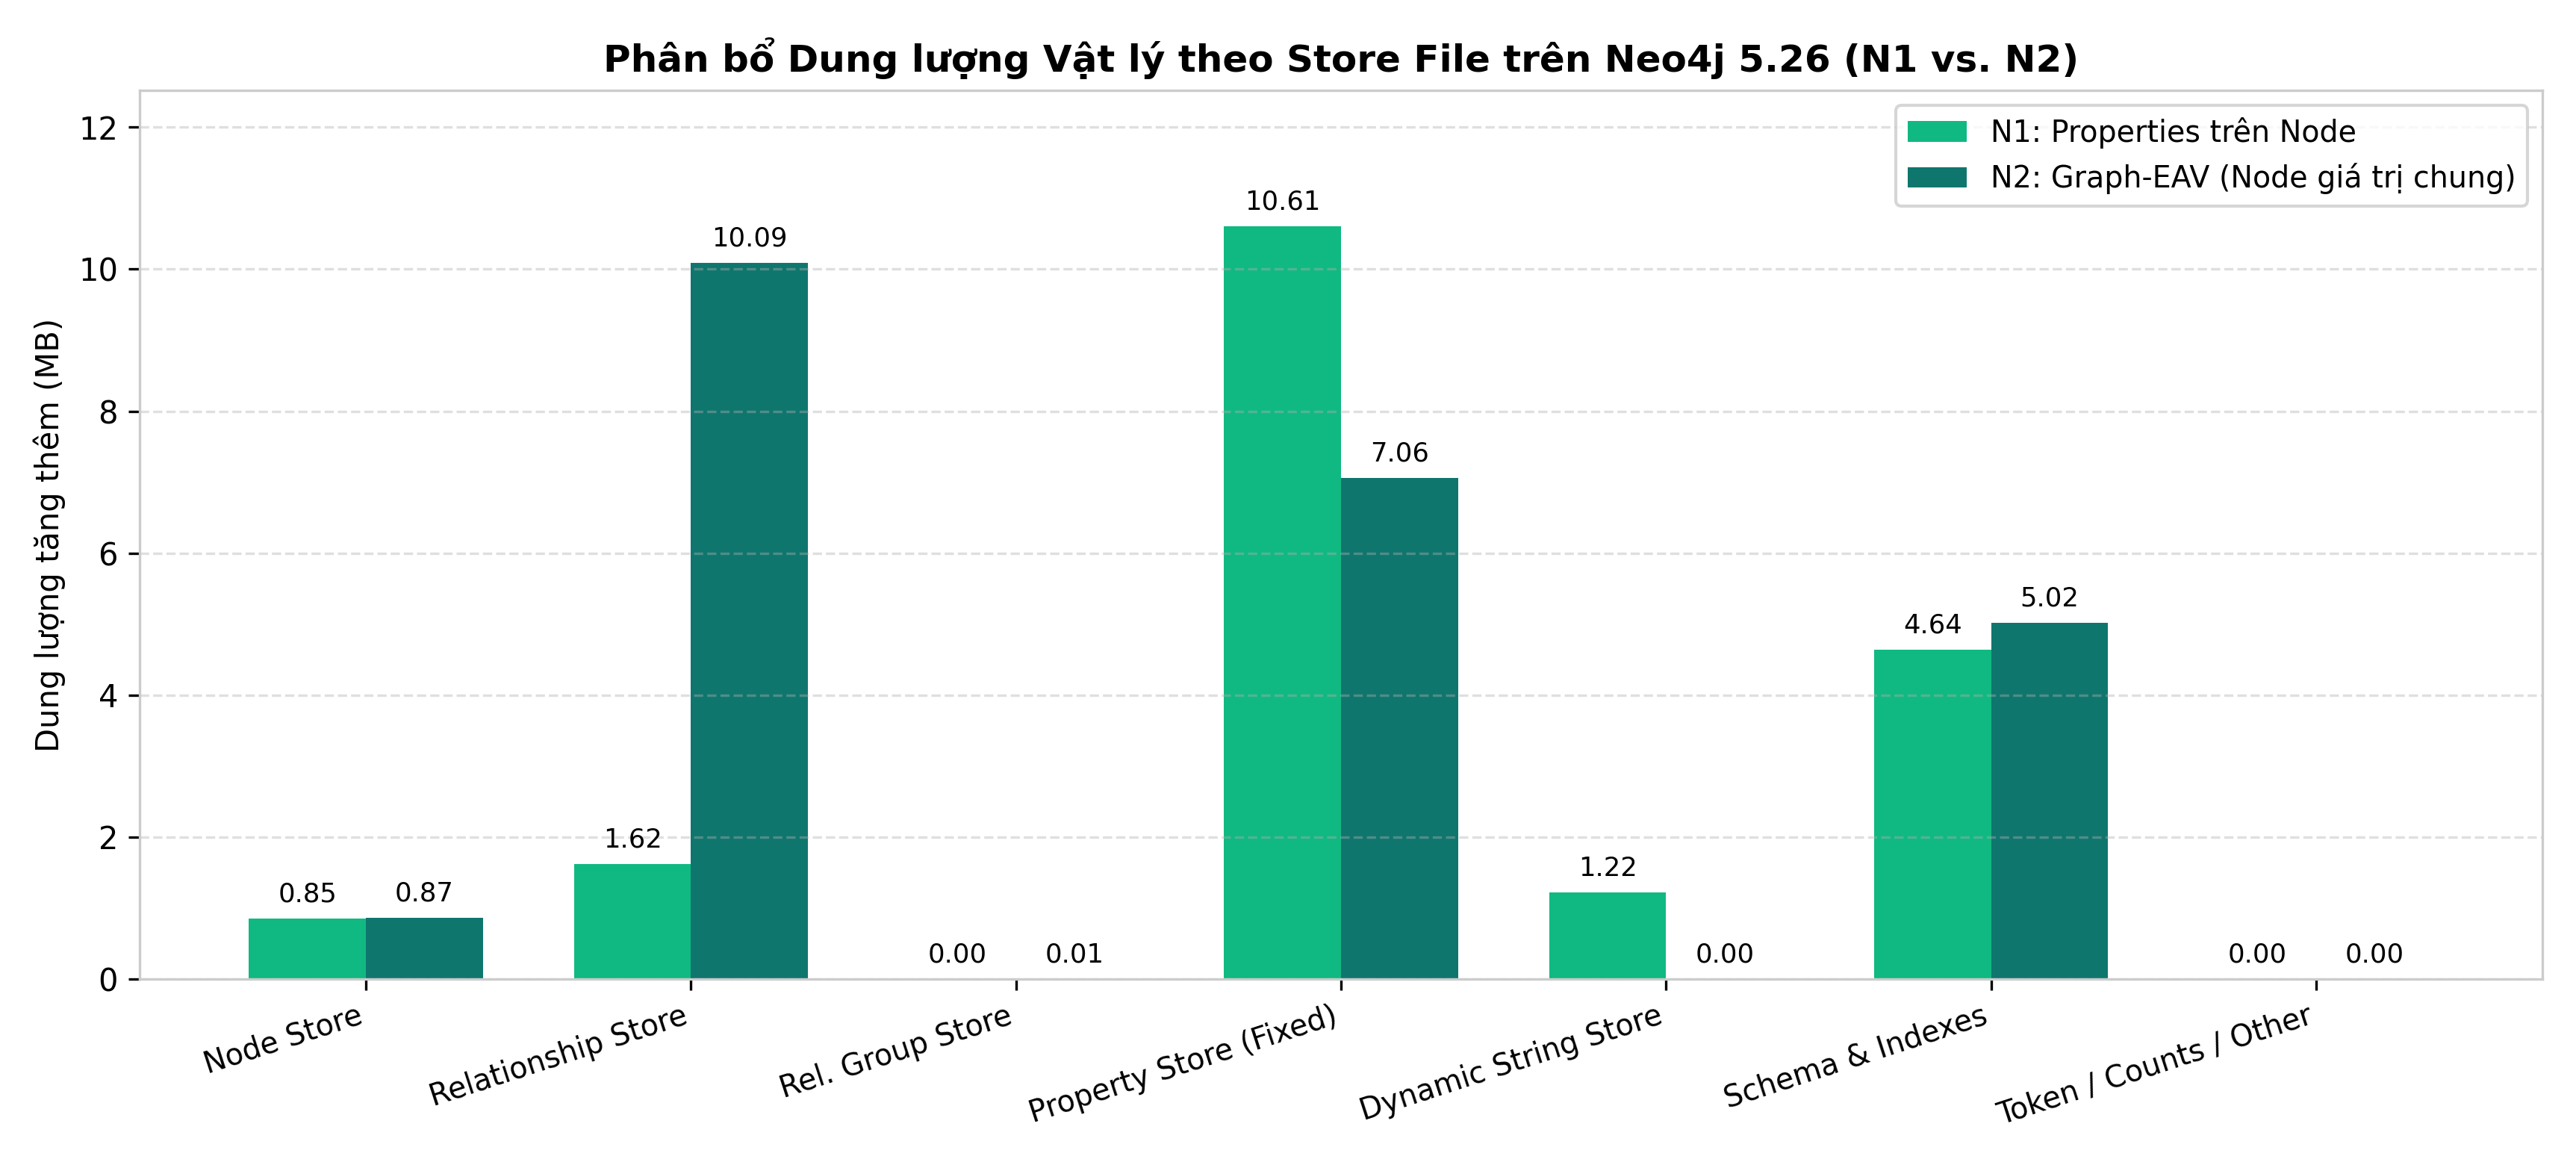
\includegraphics[width=0.95\textwidth]{report/images/topic1_neo4j_store_breakdown.png}
  \caption{Phân bổ dung lượng vật lý theo Store File trên Neo4j 5.26 (N1 vs. N2)}
  \label{fig:t1_neo4j_stores}
\end{figure}

Số liệu đo tại Bảng~\ref{tab:t1_neo4j_stores} và Hình~\ref{fig:t1_neo4j_stores} cho thấy rõ sự dịch chuyển dung lượng giữa các Store File: mô hình \texttt{N1} giữ thuộc tính trên nút làm \texttt{propertystore\_fixed} tăng \textbf{10,61 MB} và \texttt{propertystore\_strings} tăng \textbf{1,22 MB} (do lặp lại 10.000 chuỗi \texttt{isbn\_note}); ngược lại \texttt{N2} (Graph-EAV) triệt tiêu hoàn toàn phần tăng thêm của \texttt{propertystore\_strings} (\textbf{0,00 MB}) nhờ dùng chung nút giá trị, nhưng đẩy mạnh \texttt{relationshipstore} lên \textbf{10,09 MB} để lưu 260.000 cạnh \texttt{[:T1\_HAS\_ATTR]}. Đồng thời, thí nghiệm \textit{Space Reuse} trên 1.000 nút \texttt{:T1DeleteDemo} ghi nhận kích thước tổng trước khi chèn là \textbf{45.457.408 bytes} (\texttt{nodestore = 1.900.544 bytes}), sau khi chèn và checkpoint tăng lên \textbf{46.080.000 bytes} (\texttt{nodestore = 1.916.928 bytes}), và sau khi xóa bằng \texttt{DETACH DELETE} rồi checkpoint lại vẫn giữ mức \textbf{46.096.384 bytes} (\texttt{nodestore = 1.916.928 bytes}), xác nhận tệp vật lý không tự co lại ngay sau khi xóa dữ liệu.

\paragraph{Kịch bản 2: So sánh dung lượng lưu trữ vật lý trên 50.000 biến thể sản phẩm:}
Kịch bản 2 đối chiếu tổng không gian lưu trữ vật lý khi chứa cùng 50.000 biến thể đa ngành hàng giữa 6 mô hình SQL Server (đo từ \texttt{sys.partitions}, \texttt{sys.allocation\_units}, \texttt{sys.dm\_db\_index\_physical\_stats}) và 2 mô hình Neo4j:

\begin{lstlisting}[language=SQL, caption={Trích lược đồ EAV nén PAGE, Native JSON 2025 và SPARSE NULL}, label={lst:t1_sql_models}]
-- M1_EAV_PageComp: EAV value table + covering index with DATA_COMPRESSION = PAGE
CREATE TABLE dbo.T1_Variant_Attr_Values_PageComp (
    variant_id INT NOT NULL, attr_id INT NOT NULL, attr_value NVARCHAR(200) NOT NULL,
    CONSTRAINT PK_T1_EAV_PC PRIMARY KEY CLUSTERED (variant_id, attr_id)
        WITH (DATA_COMPRESSION = PAGE)
);
CREATE NONCLUSTERED INDEX IX_T1_EAV_PC_AttrVal
ON dbo.T1_Variant_Attr_Values_PageComp (attr_id, attr_value)
WITH (DATA_COMPRESSION = PAGE);

-- M2b_JsonNative: Hybrid Relational + Native `json` data type (SQL Server 2025)
CREATE TABLE dbo.T1_Variants_JsonNative (
    variant_id INT NOT NULL PRIMARY KEY CLUSTERED, product_id INT NOT NULL,
    category_name NVARCHAR(30) NOT NULL, sku NVARCHAR(40) NOT NULL,
    price DECIMAL(18,2) NOT NULL, stock_qty INT NOT NULL,
    attributes json NOT NULL
);

-- M3_Sparse: Wide Table with SPARSE NULL columns (0 bytes per NULL value)
CREATE TABLE dbo.T1_Variants_Sparse (
    variant_id INT NOT NULL PRIMARY KEY CLUSTERED, product_id INT NOT NULL,
    category_name NVARCHAR(30) NOT NULL, sku NVARCHAR(40) NOT NULL,
    price DECIMAL(18,2) NOT NULL, stock_qty INT NOT NULL,
    color NVARCHAR(20) NULL, storage_gb INT SPARSE NULL, ram_gb INT SPARSE NULL,
    cpu_model NVARCHAR(40) SPARSE NULL, apparel_size NVARCHAR(10) SPARSE NULL,
    isbn_note NVARCHAR(200) SPARSE NULL -- 20 sparse category columns in total
);
\end{lstlisting}

\begin{table}[htbp]
  \centering
  \scriptsize
  \setlength{\tabcolsep}{3.5pt}
  \renewcommand{\arraystretch}{1.25}
  \setlength{\emergencystretch}{2em}
  \caption{So sánh dung lượng lưu trữ vật lý trên 50.000 biến thể sản phẩm (8 mô hình)}
  \label{tab:t1_storage_50k}
  \begin{tabular}{|p{3.4cm}|p{2.35cm}|p{1.35cm}|p{1.4cm}|p{1.4cm}|p{1.0cm}|p{1.3cm}|}
    \hline
    \textbf{Mô hình lưu trữ} & \textbf{DBMS} & \textbf{Data (MB)} & \textbf{Index (MB)} & \textbf{Total (MB)} & \textbf{B/Var} & \textbf{In-Row Pages} \\
    \hline
    \texttt{M3\_Sparse} (SPARSE)       & SQL Server 2025 & 10,203 &  0,000 & \textbf{10,203} & 214,0 & 1.306 \\ \hline
    \texttt{M1\_EAV\_PageComp}         & SQL Server 2025 &  7,031 &  3,305 & \textbf{10,336} & 216,8 & 1.323 \\ \hline
    \texttt{Control\_WideNoSparse}     & SQL Server 2025 & 10,828 &  0,000 & \textbf{10,828} & 227,1 & 1.386 \\ \hline
    \texttt{M2b\_JsonNative}           & SQL Server 2025 & 14,133 &  0,000 & \textbf{14,133} & 296,4 & 1.809 \\ \hline
    \texttt{M2a\_JsonText}             & SQL Server 2025 & 16,648 &  0,000 & \textbf{16,648} & 349,1 & 2.131 \\ \hline
    \texttt{N1\_Neo4j\_Properties}     & Neo4j 5.26      & 14,305 &  4,641 & \textbf{18,945} & 397,3 & --    \\ \hline
    \texttt{N2\_Neo4j\_GraphEAV}       & Neo4j 5.26      & 18,031 &  5,023 & \textbf{23,055} & 483,5 & --    \\ \hline
    \texttt{M1\_EAV} (Không nén)       & SQL Server 2025 & 13,516 & 11,250 & \textbf{24,766} & 519,4 & 3.170 \\ \hline
  \end{tabular}
\end{table}

\begin{figure}[H]
  \centering
  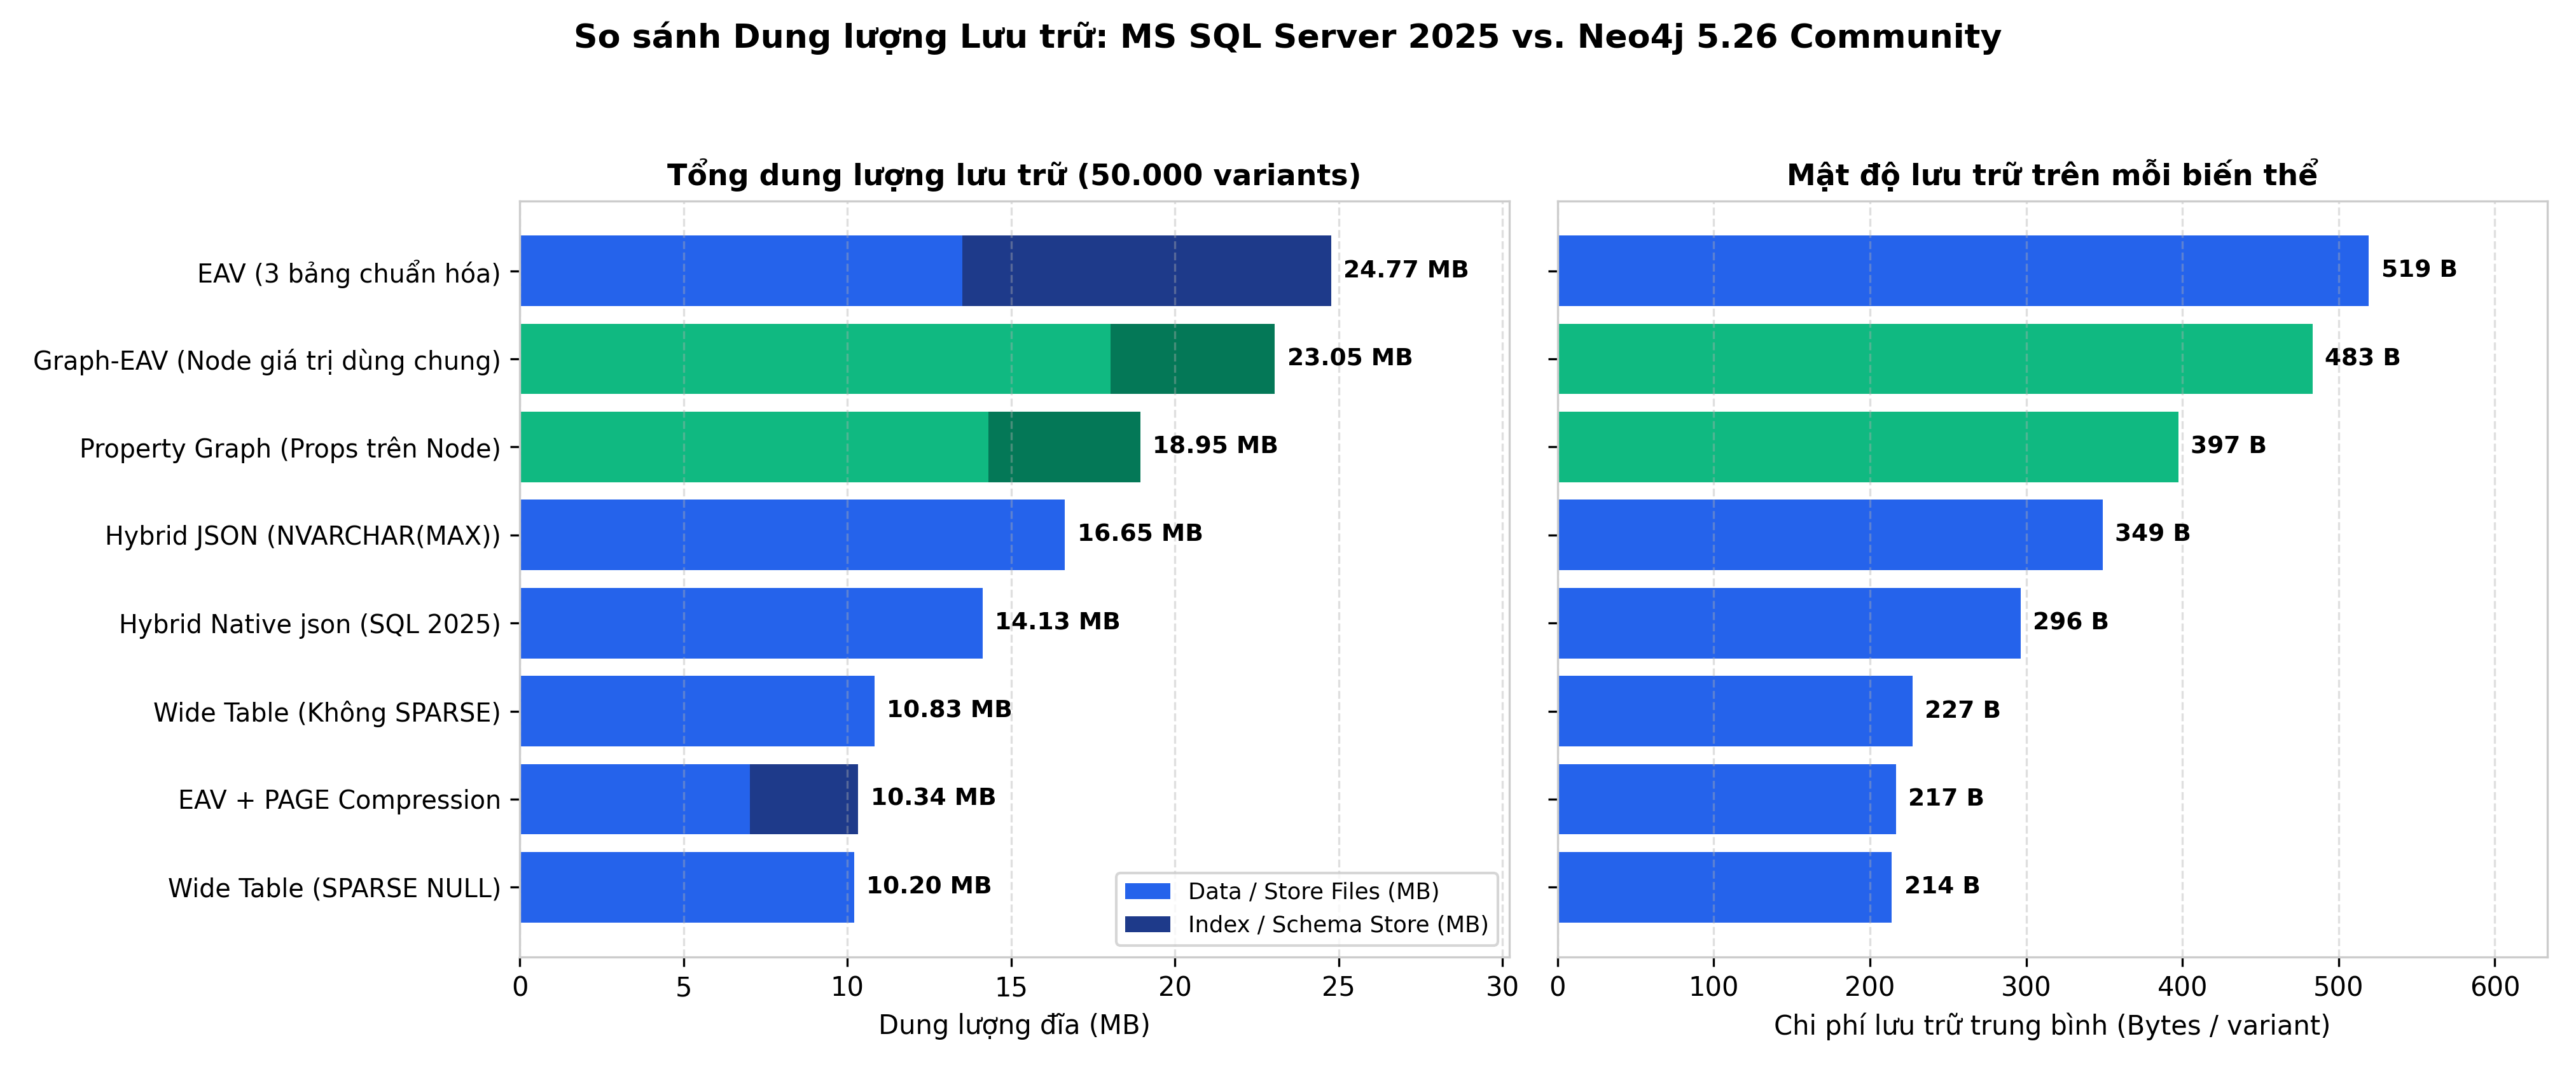
\includegraphics[width=\textwidth]{report/images/topic1_storage_comparison.png}
  \caption{So sánh tổng dung lượng đĩa và mật độ lưu trữ trên mỗi biến thể (50.000 variants)}
  \label{fig:t1_storage_comp}
\end{figure}

Kết quả tại Bảng~\ref{tab:t1_storage_50k} và Hình~\ref{fig:t1_storage_comp} (tất cả bảng SQL đều có 0 trang \texttt{ROW\_OVERFLOW\_DATA} và 0 trang \texttt{LOB\_DATA}) cho thấy bốn điểm nổi bật:
\begin{enumerate}
  \item \textbf{Tác động của nén \texttt{PAGE} lên EAV:} Khi không nén, \texttt{M1\_EAV} tốn nhiều dung lượng nhất (\textbf{24,77 MB}, 519,4 B/biến thể) do nhân thành 260.000 dòng dọc kèm chỉ mục phụ chiếm 11,25 MB. Khi bật \texttt{DATA\_COMPRESSION = PAGE}, nén từ điển và tiền tố nội trang kéo tổng dung lượng giảm \textbf{58,3\%} xuống còn \textbf{10,34 MB} (từ 3.170 xuống 1.323 trang 8 KB).
  \item \textbf{Ưu thế của kiểu \texttt{json} gốc trên SQL Server 2025:} Nhờ lưu nhị phân đã phân tích cú pháp sẵn, \texttt{M2b\_JsonNative} chỉ tiêu tốn \textbf{14,13 MB} (286,37 B/dòng), tiết kiệm trực tiếp \textbf{15,1\%} dung lượng so với \texttt{M2a\_JsonText} lưu văn bản UTF-16 (\textbf{16,65 MB}, 333,79 B/dòng).
  \item \textbf{Hiệu quả thực tế của \texttt{SPARSE NULL}:} Với tỷ lệ \texttt{NULL} 80\% trên 20 cột đặc thù, mô hình \texttt{M3\_Sparse} đạt dung lượng nhỏ nhất (\textbf{10,20 MB}), tiết kiệm \textbf{5,8\%} so với bảng đối chứng \texttt{Control\_WideNoSparse} (\textbf{10,83 MB}) do phần lớn cột chuỗi biến thiên \texttt{NVARCHAR} vốn đã nhỏ gọn khi \texttt{NULL} trong khi cột Sparse phải bù thêm chi phí \textit{Sparse Vector} cho các giá trị khác \texttt{NULL}.
  \item \textbf{Chi phí cấu trúc của Neo4j:} Cả \texttt{N1} (\textbf{18,95 MB}) và \texttt{N2} (\textbf{23,05 MB}) đều lớn hơn các mô hình lai JSON và Sparse của SQL Server vì phải lưu thêm các tệp con trỏ quan hệ hai chiều và chỉ mục nhãn (\texttt{schema\_indexes} chiếm 4,64--5,02 MB).
\end{enumerate}

\paragraph{Kịch bản 3: So sánh khả năng mở rộng Schema (Schema Evolution) và hiệu năng truy vấn (d), (a), (c):}
Kịch bản 3 kiểm tra tốc độ thích ứng khi nghiệp vụ thay đổi và hiệu năng trên nhóm truy vấn thuộc phạm vi Thành viên 1: (1) bổ sung thuộc tính mới \texttt{battery\_mAh = 5000} cho toàn bộ \textbf{10.000 biến thể Smartphones}; (2) chạy \textbf{Truy vấn (d)} điều kiện đơn lọc \texttt{color = 'Black'} (khớp chính xác \textbf{8.000 biến thể} ở cả 8 mô hình, đo trung bình 3 lần sau warmup kèm \texttt{logical reads} / \texttt{PROFILE db hits}); và (3) chạy \textbf{Truy vấn (a)} chèn thuộc tính lạ \texttt{waterproof\_ip = 'IP68'} cùng \textbf{Truy vấn (c)} cập nhật giá và màu cho \texttt{variant\_id = 1}:

\begin{lstlisting}[language=SQL, caption={Thực nghiệm Schema Evolution và truy vấn (d)/(a)/(c) trên MS SQL Server 2025}, label={lst:t1_sql_evo}]
-- 1. Schema Evolution: Wide/Sparse require DDL ALTER TABLE (Sch-M lock)
ALTER TABLE dbo.T1_Variants_Sparse ADD battery_mAh INT SPARSE NULL;
UPDATE dbo.T1_Variants_Sparse
SET battery_mAh = 5000 WHERE category_name = N'Smartphones';

--    Hybrid Native json adds attribute via DML .modify() with ZERO DDL
UPDATE dbo.T1_Variants_JsonNative
SET attributes.modify('$.battery_mAh', 5000)
WHERE category_name = N'Smartphones';

-- 2. Query (d) Single Condition: filter color = 'Black' (8,000 matches)
SELECT COUNT(*) FROM dbo.T1_Variant_Attr_Values_PageComp v
JOIN dbo.T1_Attributes a ON a.attr_id = v.attr_id
WHERE a.attr_name = N'color' AND v.attr_value = N'Black';

SELECT COUNT(*) FROM dbo.T1_Variants_JsonNative
WHERE JSON_VALUE(attributes, '$.color') = N'Black';

-- 3. Query (a) Insert novel attribute & Query (c) Point Update (FR-07)
INSERT INTO dbo.T1_Variants_JsonNative
VALUES (999999, 1, N'Smartphones', N'SKU-DEMO-IP68', 1199.00, 15,
        '{"color":"Black","waterproof_ip":"IP68"}');
UPDATE dbo.T1_Variants_JsonNative
SET price = price + 10.00, attributes.modify('$.color', N'Matte Black')
WHERE variant_id = 1;
\end{lstlisting}

\begin{lstlisting}[language={}, caption={Thực nghiệm Schema Evolution và truy vấn (d)/(a)/(c) trên Neo4j 5}, label={lst:t1_neo_evo}, morekeywords={MATCH,SET,RETURN,count,MERGE,WITH,PROFILE,WHERE,CREATE}, sensitive=false, morecomment={[l]{//}}, morestring={[b]'}]
// 1. Schema Evolution: N1 (SET property, 0 DDL) & N2 (Shared node + 10k edges)
MATCH (v:T1VariantProp {category: 'Smartphones'})
SET v.battery_mAh = 5000 RETURN count(v);

MERGE (a:T1AttrValue {name: 'battery_mAh', value: '5000'})
WITH a MATCH (v:T1VariantGraph {category: 'Smartphones'})
MERGE (v)-[:T1_HAS_ATTR]->(a) RETURN count(v);

// 2. Query (d) Single Condition: LabelScan (N1) vs Index-Free Adjacency (N2)
PROFILE MATCH (v:T1VariantProp) WHERE v.color = 'Black' RETURN count(v);
PROFILE MATCH (:T1AttrValue {name: 'color', value: 'Black'})
              <-[:T1_HAS_ATTR]-(v:T1VariantGraph)
RETURN count(v);

// 3. Query (a) Insert novel property & Query (c) Point Update
MATCH (p:T1Product {product_id: 1})
CREATE (p)-[:T1_HAS_VARIANT]->(:T1VariantProp {
  variant_id: 999999, sku: 'SKU-DEMO-IP68', price: 1199.0,
  color: 'Black', waterproof_ip: 'IP68'
});
MATCH (v:T1VariantProp {variant_id: 1})
SET v.price = v.price + 10.0, v.color = 'Matte Black';
\end{lstlisting}

\begin{table}[htbp]
  \centering
  \scriptsize
  \setlength{\tabcolsep}{3.5pt}
  \renewcommand{\arraystretch}{1.25}
  \setlength{\emergencystretch}{2em}
  \caption{Kết quả thực nghiệm Schema Evolution (10.000 Smartphones) và Truy vấn (d) (8.000 kết quả)}
  \label{tab:t1_evo_query}
  \begin{tabular}{|p{3.3cm}|p{1.2cm}|p{1.1cm}|p{1.9cm}|p{2.4cm}|p{2.1cm}|}
    \hline
    \textbf{Mô hình} & \textbf{Evo (ms)} & \textbf{Qd (ms)} & \textbf{Chi phí đọc} & \textbf{Linh hoạt Schema} & \textbf{An toàn kiểu} \\
    \hline
    \texttt{M1\_EAV}               &   645,12 &          2,03 &     32 \textit{reads} & Cao (Không DDL)         & Yếu (\texttt{NVARCHAR}) \\ \hline
    \texttt{M1\_EAV\_PageComp}     &   737,39 & \textbf{1,06} & \textbf{13 \textit{reads}} & Cao (Không DDL)    & Yếu (\texttt{NVARCHAR}) \\ \hline
    \texttt{M2a\_JsonText}         &   563,72 &        267,00 &  2.887 \textit{reads} & Cao (\texttt{JSON\_\allowbreak MODIFY}) & TB (\texttt{ISJSON}) \\ \hline
    \texttt{M2b\_JsonNative}       &   426,33 &        267,87 &  3.611 \textit{reads} & Cao (\texttt{.modify()}) & TB (Native JSON) \\ \hline
    \texttt{M3\_Sparse}            &   366,21 &         14,84 &  1.904 \textit{reads} & Thấp (DDL \texttt{Sch-M}) & Mạnh (Định kiểu) \\ \hline
    \texttt{Control\_WideNoSparse} &   304,63 &         13,61 &  1.474 \textit{reads} & Thấp (DDL \texttt{Sch-M}) & Mạnh (Định kiểu) \\ \hline
    \texttt{N1\_Neo4j\_Properties} &   758,00 &        123,33 & 100.001 \textit{hits} & Rất cao (0 DDL)         & Yếu (Community) \\ \hline
    \texttt{N2\_Neo4j\_GraphEAV}   & 1.854,00 &         80,33 & 16.004 \textit{hits}  & Rất cao (0 DDL)         & TB (\texttt{AttrValue}) \\ \hline
  \end{tabular}
\end{table}

\begin{figure}[H]
  \centering
  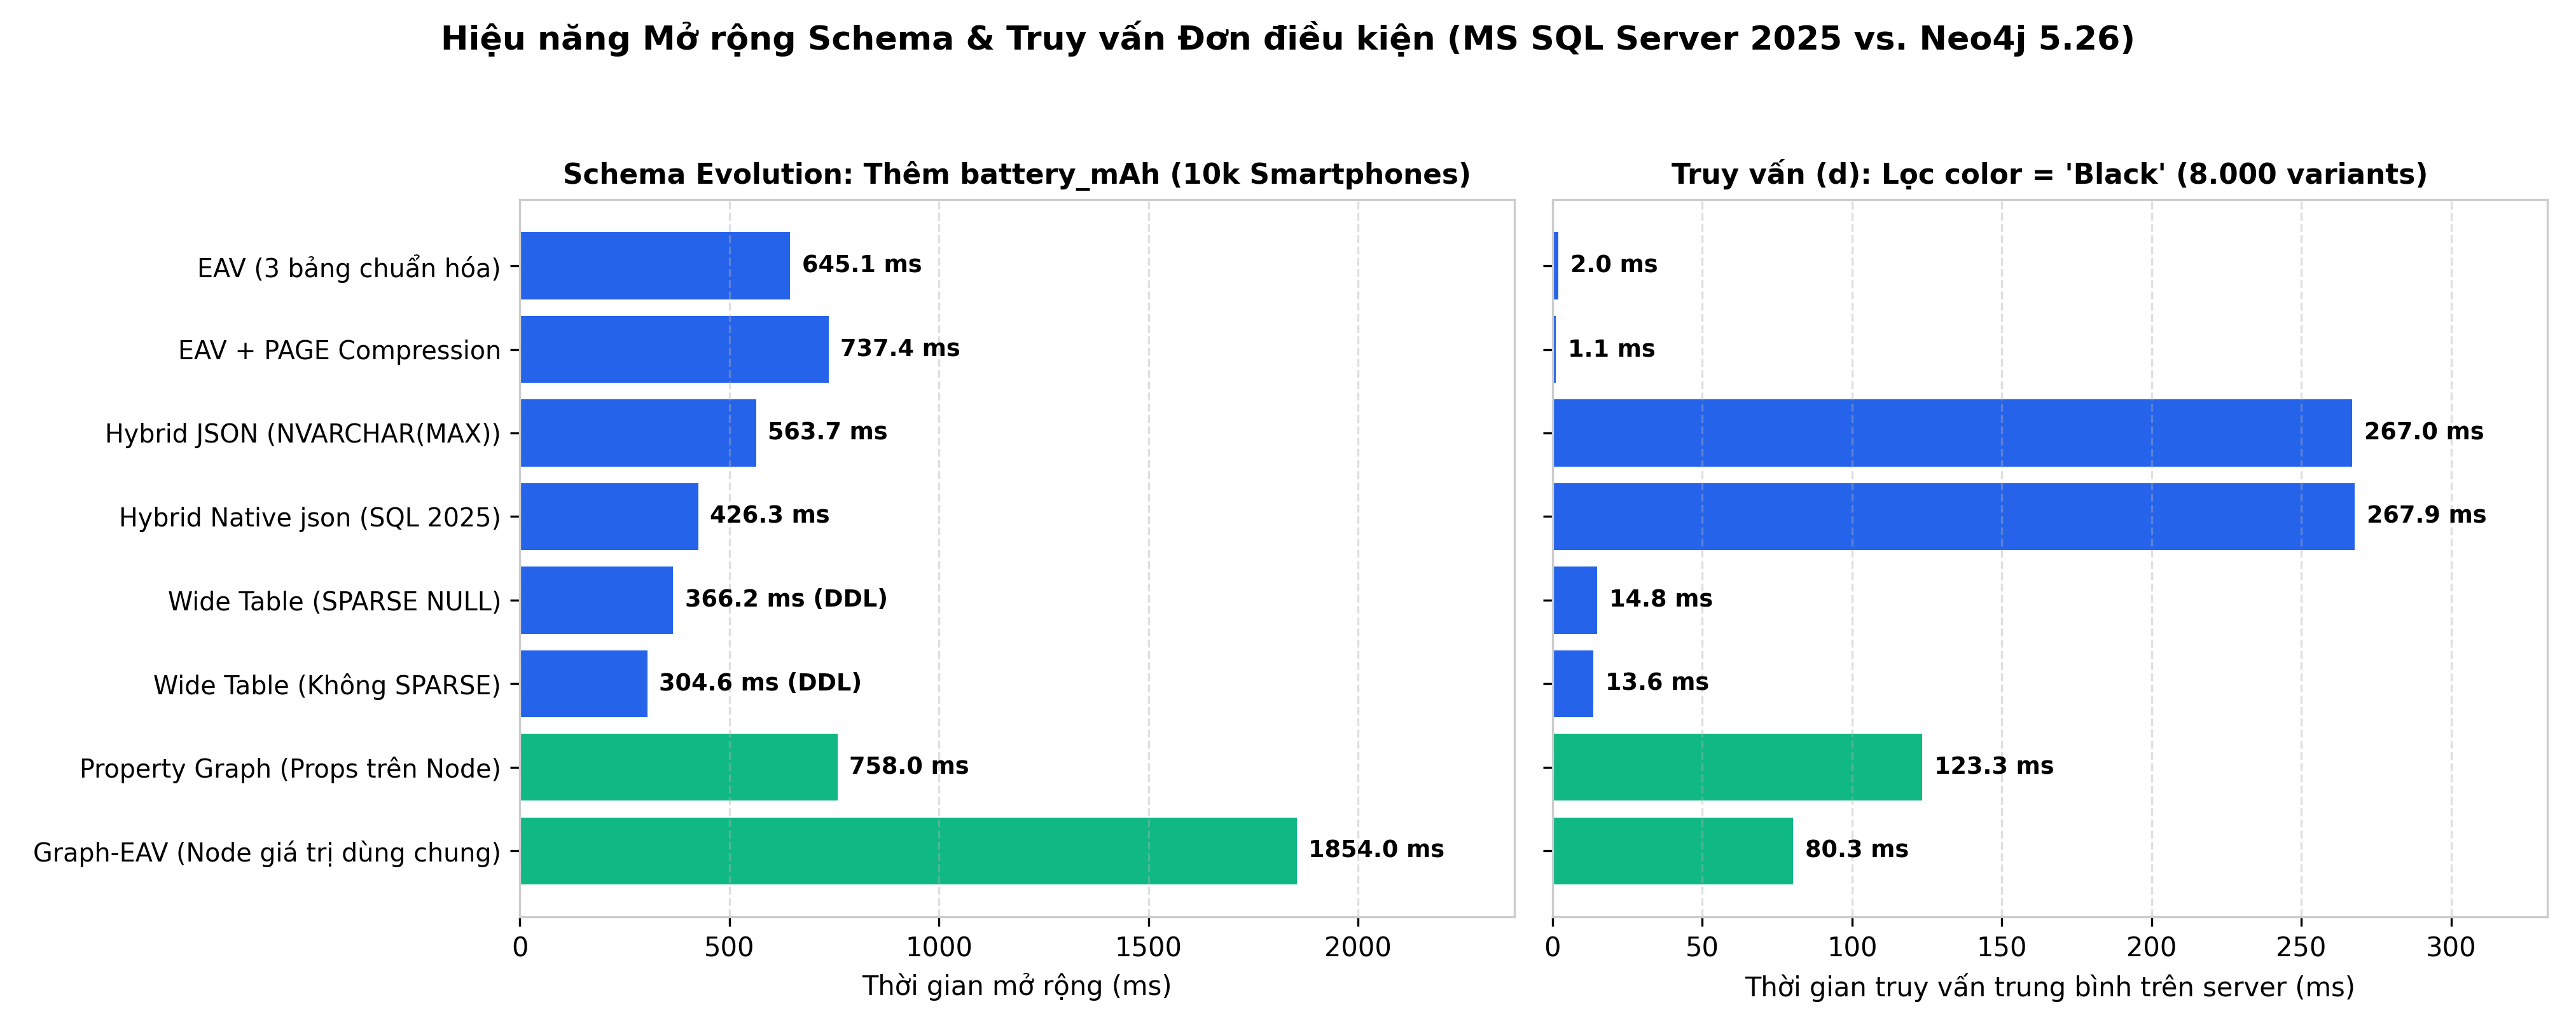
\includegraphics[width=\textwidth]{report/images/topic1_evolution_query.png}
  \caption{Hiệu năng mở rộng Schema và truy vấn đơn điều kiện (MS SQL Server 2025 vs. Neo4j 5.26)}
  \label{fig:t1_evo_query}
\end{figure}

Từ kết quả ở Bảng~\ref{tab:t1_evo_query} và Hình~\ref{fig:t1_evo_query}, có thể phân tích rõ các đánh đổi sau:
\begin{itemize}
  \item \textbf{Mở rộng Schema (\texttt{battery\_mAh}):} Hai bảng rộng \texttt{M3\_Sparse} (366,21 ms) và \texttt{Control\_WideNoSparse} (304,63 ms) phải dùng \texttt{ALTER TABLE} chiếm khóa \textbf{\texttt{Sch-M} (Schema Modification Lock)}, có nguy cơ chặn các giao dịch đồng thời trên hệ thống lớn. Ngược lại, \texttt{M2b\_JsonNative} hoàn tất mở rộng bằng DML \texttt{.modify()} trong \textbf{426,33 ms} (nhanh hơn 24,4\% so với \texttt{JSON\_MODIFY} của \texttt{M2a} ở mức 563,72 ms) mà không cần DDL. Trên Neo4j, \texttt{N1} mở rộng rất gọn bằng \texttt{SET} (758,00 ms), còn \texttt{N2} tốn 1.854,00 ms vì phải tạo mới 10.000 cạnh quan hệ trong \texttt{Relationship Store}.
  \item \textbf{Truy vấn (d) (\texttt{color = 'Black'}):} \texttt{M1\_EAV\_PageComp} đạt tốc độ nhanh nhất (\textbf{1,06 ms}, chỉ \textbf{13 logical reads}) nhờ chỉ mục bao phủ nén \texttt{PAGE}. Hai mô hình JSON chưa tạo chỉ mục computed column phải quét toàn bảng và phân tích JSON nên mất 267,00--267,87 ms. Trên Neo4j, \texttt{N2\_Neo4j\_GraphEAV} (\textbf{80,33 ms}, \textbf{16.004 db hits}) giảm được \textbf{84\% số lần truy cập CSDL} so với \texttt{N1} (\textbf{123,33 ms}, \textbf{100.001 db hits}) do \texttt{N1} phải quét toàn bộ 50.000 nút (\texttt{NodeByLabelScan}), còn \texttt{N2} định vị trực tiếp nút \texttt{:T1AttrValue} và đi theo 8.000 cạnh liền kề bằng \textit{Index-Free Adjacency}.
  \item \textbf{Truy vấn (a) Insert \& (c) Update (FR-07):} Khi thử chèn biến thể mới có thuộc tính lạ \texttt{waterproof\_ip = 'IP68'}, mô hình \texttt{M3\_Sparse} lập tức bị từ chối với lỗi \textbf{Msg 207} (\textit{Invalid column name 'waterproof\_ip'}), thể hiện tính khắt khe của \textit{Schema-on-Write}; trong khi \texttt{M2b\_JsonNative} chèn thành công trong \textbf{5,88 ms} và cập nhật giá + màu cục bộ bằng \texttt{.modify()} chỉ mất \textbf{3,00 ms}. Trên Neo4j, lệnh Cypher đơn lẻ tạo thuộc tính mới kèm dọn dẹp ghi nhận \textbf{669,00 ms} và lệnh cập nhật + khôi phục ghi nhận \textbf{307,00 ms} (do là lượt chạy đơn chưa làm nóng bộ đệm kế hoạch thực thi và bao gồm thao tác dọn dẹp trong cùng phiên \texttt{cypher-shell}).
\end{itemize}

\subsubsection{Đánh giá và quyết định}

Bảng~\ref{tab:t1_summary} tổng hợp các đặc tính cốt lõi về lưu trữ và quản trị dữ liệu giữa MS SQL Server 2025 và Neo4j 5.26:

\begin{table}[htbp]
  \centering
  \footnotesize
  \setlength{\tabcolsep}{4pt}
  \renewcommand{\arraystretch}{1.25}
  \setlength{\emergencystretch}{2em}
  \caption{So sánh tổng hợp cơ chế Data Storage \& Management giữa MS SQL Server và Neo4j}
  \label{tab:t1_summary}
  \begin{tabular}{|p{2.9cm}|p{5.0cm}|p{5.0cm}|}
    \hline
    \textbf{Tiêu chí} & \textbf{MS SQL Server (2025)} & \textbf{Neo4j (5.26 LTS)} \\
    \hline
    Mô hình dữ liệu & Relational Model & Labeled Property Graph \\ \hline
    Thiết kế Schema & Schema-on-Write (ép ràng buộc khi ghi) & Schema-Optional (linh hoạt thuộc tính) \\ \hline
    Tổ chức dữ liệu & Tables, Rows, Columns & Nodes, Relationships, Properties \\ \hline
    Đơn vị lưu trữ & Page 8 KB, Extent 64 KB & Record Store (Aligned) hoặc Block Store \\ \hline
    Cấu trúc lưu trữ & Heap, Clustered Index B+Tree & Node, Relationship, Property Store \\ \hline
    Truy xuất quan hệ & Foreign Key và JOIN & Index-Free Adjacency ($O(1)$/bước nhảy) \\ \hline
    Dữ liệu lớn / động & Row Overflow, LOB, Native \texttt{json}, Sparse & Inline Storage và Dynamic Storage \\ \hline
    Bộ nhớ đệm & Buffer Pool & Off-Heap Page Cache (tách JVM Heap) \\ \hline
    Cơ chế nén & Row Compression, Page Compression & Phụ thuộc Store Format \\ \hline
    Mở rộng thuộc tính & \texttt{ALTER TABLE} (\texttt{Sch-M}) hoặc EAV/JSON & \texttt{SET}/\texttt{CREATE} tức thì (0 DDL) \\ \hline
    Phục hồi dữ liệu & Transaction Log, Checkpoint, REDO/UNDO & Transaction Log, Checkpoint, Recovery \\ \hline
    Thu hồi không gian & Ghost Cleanup, REBUILD, REORGANIZE & Space Reuse và Defragmentation \\ \hline
  \end{tabular}
\end{table}

\paragraph{Quyết định lựa chọn cho hệ thống E-Commerce:} Từ phân tích lý thuyết và số liệu thực nghiệm trên, nhóm quyết định chọn \textbf{MS SQL Server} làm hệ quản trị cơ sở dữ liệu chính cho nền tảng thương mại điện tử đa gian hàng vì ba lý do then chốt:

\begin{enumerate}
  \item \textbf{Bảo toàn tính toàn vẹn bằng Schema-on-Write:} Hệ thống E-Commerce xoay quanh các thực thể giao dịch tài chính và tồn kho (\texttt{Users}, \texttt{Sellers}, \texttt{Products}, \texttt{Orders}, \texttt{Order\_Details}, \texttt{Vouchers}), đòi hỏi cơ chế kiểm tra kiểu dữ liệu, khóa ngoại và ràng buộc \texttt{CHECK} nghiêm ngặt ngay tại tầng Storage Engine (như đã chứng minh bằng lỗi 547 khi chặn giá âm).
  \item \textbf{Hiệu quả nén và lưu trữ đa dạng trên trang 8 KB:} Kiến trúc Page 8 KB kết hợp \texttt{DATA\_COMPRESSION = PAGE} (216,8 B/biến thể) và mô hình lai Native \texttt{json} (296,4 B/biến thể, 0 DDL khi mở rộng) giúp tối ưu dung lượng đĩa vượt trội so với Neo4j (397,3--483,5 B/biến thể), vừa giữ trọn lợi thế quan hệ vừa linh hoạt cho biến thể sản phẩm.
  \item \textbf{Khả năng kết hợp Polyglot Persistence trong tương lai:} Neo4j không phù hợp thay thế cho CSDL giao dịch chính do thiếu chuẩn hóa ràng buộc bảng, nhưng rất lý tưởng để vận hành song song cho các phân hệ phân tích đồ thị nhiều tầng như hệ thống gợi ý sản phẩm cá nhân hóa hoặc phát hiện gian lận liên kết giữa \texttt{Users} -- \texttt{Orders} -- \texttt{Sellers}.
\end{enumerate}


% ==============================================================================
% CÁC ĐOẠN CẦN BỔ SUNG VÀO CÁC VỊ TRÍ KHÁC TRONG main.tex (BỎ COMMENT KHI DÁN)
% ==============================================================================
%
% --- [1] Dòng bổ sung vào Bảng 1 (Danh sách thành viên & Phân công công việc) ---
% 2 & Trần Quốc Hiền & 2310992 &
%   - Nghiên cứu chủ đề Data Storage \& Schema Design (MS SQL Server vs Neo4j) \newline
%   - Thiết kế lược đồ ECommerceDB và hiện thực FR-02, FR-07, AuthModule & 100\% \\ \hline
%
% --- [2] Sửa lỗi tiêu đề "Tài liệu" bị cắt chữ ở cuối main.tex (nếu dùng babel vietnamese) ---
% Thêm dòng này trước \begin{document} trong main.tex:
% \addto\captionsvietnamese{\renewcommand{\refname}{Tài liệu tham khảo}}
%
% --- [3] 9 Tài liệu tham khảo nối tiếp sau [10] trong \begin{thebibliography} ---
% \bibitem{t1_date2004}
% C.~J. Date, \textit{An Introduction to Database Systems}, 8th~ed. Pearson, 2004.
%
% \bibitem{t1_silberschatz2019}
% A.~Silberschatz, H.~F. Korth, and S.~Sudarshan, \textit{Database System Concepts}, 7th~ed. McGraw-Hill, 2019.
%
% \bibitem{t1_delaney2012}
% K.~Delaney et~al., \textit{Microsoft SQL Server 2012 Internals}. Microsoft Press, 2012.
%
% \bibitem{t1_mspages}
% Microsoft Learn, \textit{Pages and Extents Architecture Guide -- SQL Server}. [Online]. Available: \url{https://learn.microsoft.com/en-us/sql/relational-databases/pages-and-extents-architecture-guide}
%
% \bibitem{t1_mssparse}
% Microsoft Learn, \textit{Use Sparse Columns -- SQL Server}. [Online]. Available: \url{https://learn.microsoft.com/en-us/sql/relational-databases/tables/use-sparse-columns}
%
% \bibitem{t1_mscomp}
% Microsoft Learn, \textit{Data Compression -- SQL Server}. [Online]. Available: \url{https://learn.microsoft.com/en-us/sql/relational-databases/data-compression/data-compression}
%
% \bibitem{t1_msnativejson}
% Microsoft Learn, \textit{JSON data type (SQL Server 2025)}. [Online]. Available: \url{https://learn.microsoft.com/en-us/sql/t-sql/data-types/json-data-type}
%
% \bibitem{t1_robinson2015}
% I.~Robinson, J.~Webber, and E.~Eifrem, \textit{Graph Databases: New Opportunities for Connected Data}, 2nd~ed. O'Reilly Media, 2015.
%
% \bibitem{t1_neo4jops}
% Neo4j Documentation, \textit{Operations Manual: Store Formats, Memory Configuration, Transaction Logs and Checkpointing}. [Online]. Available: \url{https://neo4j.com/docs/operations-manual/current/}

%      (hoặc copy-paste toàn bộ nội dung từ \subsubsection{...} đến trước phần
%      comment ở cuối file này).
%   3. Cập nhật Bảng 1 (Danh sách thành viên) và nối các \bibitem{t1_...} ở cuối
%      file này vào khối \begin{thebibliography} của main.tex.
% ==============================================================================

\subsubsection{Khái niệm chung về Data Storage và Data Management}

\textbf{Data Storage (Lưu trữ dữ liệu)} là quá trình tổ chức, cấu trúc hóa và duy trì dữ liệu dưới các định dạng nhị phân phù hợp trên thiết bị lưu trữ thứ cấp (SSD/HDD) nhằm bảo đảm độ bền lâu dài, hiệu quả truy xuất và khả năng mở rộng khi khối lượng dữ liệu gia tăng. Thành phần đảm nhiệm trực tiếp chức năng này bên trong một hệ quản trị cơ sở dữ liệu (DBMS) là \textbf{Storage Engine} -- lớp phần mềm cốt lõi chịu trách nhiệm cấp phát không gian đĩa, quản lý bộ nhớ đệm (\textit{Buffer Pool} hoặc \textit{Page Cache}) và duy trì nhật ký giao dịch (\textit{Transaction Log}) phục vụ khôi phục dữ liệu~\cite{t1_date2004,t1_silberschatz2019}.

\textbf{Data Management (Quản trị dữ liệu)} bao gồm tập hợp các cơ chế vận hành trên dữ liệu đã lưu trữ: kiểm soát toàn vẹn ngữ nghĩa và ràng buộc tham chiếu, thực thi truy vấn, xử lý giao dịch (\textit{Transaction}), điều khiển đồng thời, thu hồi không gian trống và bảo đảm tính bền vững sau sự cố. Kiến trúc lưu trữ ở tầng vật lý ảnh hưởng trực tiếp đến chi phí I/O, hiện tượng phân mảnh trang đĩa, dung lượng lưu trữ tiêu thụ cũng như mức độ linh hoạt khi nghiệp vụ thay đổi.

Trong bài toán thực tế của nhóm là nền tảng sàn thương mại điện tử đa gian hàng (\textit{Multi-Vendor E-Commerce Platform}, CSDL \texttt{ECommerceDB}), hệ thống vừa đòi hỏi tính nhất quán chặt chẽ ở các bảng giao dịch cốt lõi (\texttt{Users}, \texttt{Sellers}, \texttt{Orders}, \texttt{Order\_Details}, \texttt{Vouchers}), vừa phát sinh bài toán đặc trưng về \textbf{thuộc tính biến thể sản phẩm linh hoạt}: sản phẩm thuộc ngành hàng \textit{Smartphones} cần lưu \texttt{storage\_gb}, \texttt{ram\_gb}, \texttt{screen\_inch}, \texttt{chipset}; ngành hàng \textit{Laptops} cần \texttt{cpu\_model}, \texttt{gpu\_model}, \texttt{os\_name}; ngành hàng \textit{Fashion} cần \texttt{apparel\_size}, \texttt{material}, \texttt{fit\_style}; còn ngành hàng \textit{Books} lại cần \texttt{author\_name}, \texttt{publisher}, \texttt{page\_count} và \texttt{isbn\_note}. Cách tiếp cận bài toán này phản ánh rõ sự đối lập giữa hai triết lý thiết kế dữ liệu:

\begin{itemize}
  \item \textbf{MS SQL Server (Schema-on-Write):} Yêu cầu khai báo tường minh toàn bộ cấu trúc bảng, kiểu dữ liệu và các ràng buộc (\texttt{PRIMARY KEY}, \texttt{FOREIGN KEY}, \texttt{CHECK}, \texttt{NOT NULL}, \texttt{UNIQUE}) trước khi ghi dữ liệu. Mọi thao tác \texttt{INSERT} hoặc \texttt{UPDATE} đều được kiểm tra nghiêm ngặt ngay tại thời điểm ghi nhằm bảo đảm tính nhất quán cao.
  \item \textbf{Neo4j (Schema-Optional):} Lưu trữ theo mô hình đồ thị thuộc tính có nhãn (\textit{Labeled Property Graph}), cho phép các nút cùng nhãn mang tập thuộc tính khác nhau và bổ sung thuộc tính mới ngay trong quá trình ghi mà không cần chỉnh sửa lược đồ tĩnh, đồng thời vẫn hỗ trợ \textit{Indexes} và \textit{Constraints} để kiểm soát các khóa định danh quan trọng~\cite{t1_robinson2015,t1_neo4jops}.
\end{itemize}

\subsubsection{Đặc trưng cơ chế Data Storage và Data Management trong MS SQL Server}

\paragraph{Mô hình tổ chức và thiết kế dữ liệu cho thuộc tính động:}
MS SQL Server tổ chức dữ liệu logic dưới dạng bảng hai chiều (\textit{Tables, Rows, Columns}) và cung cấp hai cấu trúc lưu trữ vật lý nền tảng cho dữ liệu hàng (\textit{Rowstore})~\cite{t1_delaney2012,t1_mspages}:
\begin{itemize}
  \item \textbf{Heap:} Bảng không có \textit{Clustered Index}; các dòng dữ liệu được lưu tự do không theo thứ tự khóa và được định vị thông qua địa chỉ vật lý \textbf{RID} (\textit{FileID:PageID:SlotID}).
  \item \textbf{Clustered Index:} Tổ chức bảng dưới dạng cây cân bằng \textbf{B+Tree}, trong đó các nút lá chứa trực tiếp toàn bộ dữ liệu dòng được sắp xếp theo thứ tự khóa cụm (mặc định gắn với \texttt{PRIMARY KEY}).
\end{itemize}

Khi mô hình hóa tập thuộc tính biến thể đa dạng trên nền tảng chuẩn hóa quan hệ (1NF--3NF), các hệ thống dùng SQL Server thường áp dụng một trong ba hướng thiết kế sau:
\begin{itemize}
  \item \textbf{Mô hình Entity--Attribute--Value (EAV):} Tách danh mục thuộc tính sang bảng \texttt{Attributes} và lưu từng cặp thuộc tính--giá trị dưới dạng các dòng dọc trong bảng \texttt{Variant\_Attr\_Values}. EAV cho phép thêm thuộc tính mới bằng lệnh \texttt{INSERT} (không cần DDL), nhưng làm tăng mạnh số dòng dữ liệu, giảm an toàn kiểu dữ liệu (thường phải lưu chuỗi \texttt{NVARCHAR}) và phát sinh nhiều phép \texttt{JOIN} khi truy xuất nhiều thuộc tính cùng lúc.
  \item \textbf{Wide Table với Sparse Columns:} Khai báo tất cả thuộc tính của mọi ngành hàng thành các cột trên một bảng rộng kèm từ khóa \texttt{SPARSE NULL}~\cite{t1_mssparse}. Mỗi giá trị \texttt{NULL} trên cột Sparse tiêu thụ \textbf{0 byte} lưu trữ, nhưng mỗi giá trị khác \texttt{NULL} phát sinh thêm 2--4 byte chi phí quản lý trong cấu trúc \textit{Sparse Vector} (chỉ đạt hiệu quả nén khi tỷ lệ \texttt{NULL} cao, thường $\ge$ 20--40\% tùy kiểu dữ liệu) và vẫn phụ thuộc vào lệnh DDL \texttt{ALTER TABLE} khi cần thêm cột mới.
  \item \textbf{Mô hình Hybrid JSON (\texttt{NVARCHAR(MAX)} và kiểu \texttt{json} gốc trên SQL Server 2025):} Giữ các cột giao dịch cốt lõi (\texttt{variant\_id}, \texttt{product\_id}, \texttt{sku}, \texttt{price}, \texttt{stock\_qty}) dưới dạng quan hệ chuẩn định kiểu chặt chẽ, còn tập thuộc tính đặc thù theo ngành hàng được đóng gói vào cột bán cấu trúc. Trước đây, dữ liệu JSON được lưu dưới dạng chuỗi UTF-16 trong \texttt{NVARCHAR(MAX)} kèm ràng buộc \texttt{CHECK} \texttt{(ISJSON(col) = 1)} và cập nhật qua \texttt{JSON\_MODIFY()}. Từ phiên bản \textbf{MS SQL Server 2025}, hệ thống bổ sung kiểu dữ liệu \textbf{\texttt{json} gốc (Native \texttt{json} Data Type)} lưu ở định dạng nhị phân đã phân tích cú pháp sẵn (\textit{pre-parsed binary}) cùng phương thức \texttt{.modify()} trực tiếp, giúp tiết kiệm dung lượng đĩa và giảm chi phí phân tích cú pháp~\cite{t1_msnativejson}.
\end{itemize}

\paragraph{Kiến trúc tệp và trang lưu trữ (Page \& Extent):}
Ở tầng vật lý, mỗi CSDL SQL Server sử dụng ba loại tệp chính: \texttt{.mdf} (tệp dữ liệu chính), \texttt{.ndf} (tệp dữ liệu phụ) và \texttt{.ldf} (tệp nhật ký giao dịch)~\cite{t1_mspages}. Không gian bên trong tệp dữ liệu được chia nhỏ thành các đơn vị lưu trữ chuẩn hóa~\cite{t1_delaney2012,t1_mspages}:
\begin{itemize}
  \item \textbf{Page:} Đơn vị I/O cơ bản có kích thước cố định \textbf{8 KB (8.192 bytes)}, gồm ba vùng chính: (1) \textit{Page Header} (96 bytes đầu chứa mã trang \texttt{m\_pageId}, loại trang \texttt{m\_type}, số dòng \texttt{m\_slotCnt}, vùng trống \texttt{m\_freeCnt}, số bản ghi ma \texttt{m\_ghostRecCnt} và LSN gần nhất \texttt{m\_lsn}); (2) \textit{Data Area} (nơi lưu nối tiếp các dòng dữ liệu); và (3) \textit{Slot Array} ở cuối trang lưu offset trỏ về vị trí từng dòng theo thứ tự logic.
  \item \textbf{Extent:} Gồm \textbf{8 Page liên tiếp}, tương đương \textbf{64 KB}, gồm \textit{Uniform Extent} (cấp phát cho một đối tượng duy nhất) và \textit{Mixed Extent} (chia sẻ giữa tối đa 8 đối tượng nhỏ).
\end{itemize}

\paragraph{Lưu trữ dữ liệu lớn (Allocation Units) và cơ chế nén:}
SQL Server quản lý dữ liệu có kích thước thay đổi thông qua ba \textbf{Allocation Units}~\cite{t1_mspages}:
\begin{itemize}
  \item \textbf{\texttt{IN\_ROW\_DATA}:} Lưu các cột cố định và biến thiên trực tiếp trên trang dữ liệu chính với giới hạn dòng chuẩn tối đa \textbf{8.060 bytes}.
  \item \textbf{\texttt{ROW\_OVERFLOW\_DATA}:} Tự động đẩy các cột độ dài biến thiên (như \texttt{VARCHAR}, \texttt{NVARCHAR}) sang trang tràn dòng khi tổng kích thước dòng vượt quá 8.060 bytes, giữ lại con trỏ 24-byte trên trang gốc.
  \item \textbf{\texttt{LOB\_DATA}:} Lưu trữ các kiểu dữ liệu khối lớn như \texttt{VARCHAR(MAX)}, \texttt{NVARCHAR(MAX)}, \texttt{VARBINARY\allowbreak(MAX)} hoặc \texttt{json} vượt ngưỡng lưu nội dòng.
\end{itemize}

Để tối ưu dung lượng đĩa và I/O bộ nhớ đệm, SQL Server hỗ trợ hai cơ chế nén tích hợp (\texttt{DATA\_COMPRESSION})~\cite{t1_mscomp}: \textbf{Row Compression} chuyển kiểu dữ liệu cố định sang biểu diễn độ dài biến thiên theo giá trị thực và loại bỏ byte đệm trống; trong khi \textbf{Page Compression} kết hợp tuần tự \textit{Row Compression}, \textit{Prefix Compression} (trích xuất tiền tố chung của cột) và \textit{Dictionary Compression} (thay thế giá trị lặp lại toàn trang bằng từ điển nội trang).

\paragraph{Quản lý không gian, phân mảnh và Transaction Log:}
SQL Server theo dõi không gian cấp phát qua các trang bitmap chuyên biệt gồm \textbf{GAM/SGAM} (trạng thái cấp phát Extent), \textbf{PFS} (tỷ lệ chỗ trống của từng Page) và \textbf{IAM} (ánh xạ các Extent thuộc một Allocation Unit)~\cite{t1_mspages}. Khi thêm, sửa hoặc xóa dữ liệu liên tục, hệ thống có thể phát sinh \textbf{Page Split} (tách đôi trang lá B+Tree đã đầy khi chèn khóa mới), \textbf{Forwarded Record} (dòng trên bảng Heap phình to phải dời sang trang khác để lại con trỏ chuyển tiếp), và \textbf{Ghost Record} (đánh dấu logic bản ghi bị xóa hoặc hủy bỏ trên trang lá để tiến trình nền \textit{Ghost Cleanup} thu hồi sau). Quản trị viên bảo trì cấu trúc bằng \texttt{REORGANIZE}/\texttt{REBUILD} và thu hồi dung lượng tệp đĩa bằng \texttt{DBCC SHRINKFILE}. Toàn bộ biến động trên \textit{Buffer Pool} tuân thủ nguyên tắc \textbf{Write-Ahead Logging (WAL)}, kết hợp tiến trình \textbf{Checkpoint} và cơ chế \textbf{REDO/UNDO} từ Transaction Log để đảm bảo phục hồi bền vững~\cite{t1_delaney2012}.

\subsubsection{Đặc trưng cơ chế Data Storage và Data Management trong Neo4j}

\paragraph{Mô hình Labeled Property Graph:}
Neo4j lưu trữ dữ liệu trực tiếp theo mô hình \textbf{Labeled Property Graph (LPG)} gồm ba thành phần cốt lõi~\cite{t1_robinson2015,t1_neo4jops}:
\begin{itemize}
  \item \textbf{Nodes (Nút):} Đại diện cho thực thể (ví dụ \texttt{:User}, \texttt{:Product}, \texttt{:T1VariantProp}); mỗi nút có thể mang một hoặc nhiều nhãn (\textit{Labels}).
  \item \textbf{Relationships (Quan hệ):} Biểu diễn liên kết có hướng và có kiểu giữa nút nguồn và nút đích, ví dụ \texttt{(User)-[:PLACED]->(Order)} hay \texttt{(Product)-\allowbreak[:HAS\_VARIANT]->\allowbreak(Variant)}; mỗi cạnh cũng có thể mang thuộc tính riêng.
  \item \textbf{Properties (Thuộc tính):} Các cặp \textit{Key--Value} linh hoạt gắn trực tiếp lên Node hoặc Relationship.
\end{itemize}

\paragraph{Native Graph Storage và Index-Free Adjacency:}
Neo4j tổ chức dữ liệu đồ thị gốc thành các tệp store vật lý chuyên biệt có kích thước bản ghi cố định trong thư mục dữ liệu~\cite{t1_neo4jops}:
\begin{itemize}
  \item \textbf{Node Store (\texttt{neostore.nodestore.db}):} Lưu thông tin nút, nhãn và con trỏ trỏ tới quan hệ đầu tiên cùng chuỗi thuộc tính đầu tiên.
  \item \textbf{Relationship Store (\texttt{neostore.relationshipstore.db}):} Lưu nút nguồn, nút đích, loại quan hệ và chuỗi liên kết đôi đến các quan hệ kế tiếp của hai đầu nút.
  \item \textbf{Relationship Group Store (\texttt{neostore.\allowbreak relationshipgroupstore.db}):} Gom nhóm cạnh theo loại và chiều đối với các \textit{dense nodes} (nút có mật độ kết nối lớn).
  \item \textbf{Property Store (\texttt{neostore.propertystore.db}) \& Dynamic Store:} Lưu bản ghi thuộc tính cố định và tham chiếu đến vùng lưu trữ động.
\end{itemize}

Neo4j hỗ trợ nhiều \textbf{Store Format} khác nhau theo phiên bản và ấn bản: \textit{Aligned Format} là định dạng mặc định trên ấn bản Community Edition (tối ưu sắp thẳng biên trang với kích thước bản ghi nhẹ), trong khi \textit{Block Format} được sử dụng mặc định trên các phiên bản Enterprise Edition tương ứng~\cite{t1_neo4jops}. Nhờ lưu trực tiếp con trỏ cạnh ngay tại mỗi nút, Neo4j đạt được cơ chế \textbf{Index-Free Adjacency}: hệ thống duyệt qua các mối liên kết lân cận theo tham chiếu trực tiếp với chi phí $O(1)$ cho mỗi bước nhảy mà không cần tra cứu chỉ mục toàn cục như phép \texttt{JOIN} trong SQL Server~\cite{t1_robinson2015}. Tuy nhiên, nếu truy vấn lọc thuộc tính trên toàn bộ nút mà không qua cạnh hoặc chỉ mục, Neo4j vẫn phải quét nhãn (\texttt{NodeByLabelScan}).

\paragraph{Lưu trữ thuộc tính động, Page Cache và Transaction Log:}
Để cân bằng tốc độ truy cập và kích thước thuộc tính biến thiên, Neo4j kết hợp hai cơ chế lưu thuộc tính~\cite{t1_neo4jops}:
\begin{itemize}
  \item \textbf{Inline Storage:} Các giá trị nguyên thủy và chuỗi ngắn vừa kích thước khối thuộc tính được mã hóa và lưu trực tiếp trong \texttt{Property Store}, hạn chế đọc thêm tệp ngoài.
  \item \textbf{Dynamic Storage:} Các chuỗi dài hoặc mảng lớn vượt ngưỡng được tách sang tệp lưu trữ động (\texttt{.strings}, \texttt{.arrays}) và tham chiếu ngược từ bản ghi chính.
\end{itemize}

Về quản lý bộ nhớ và không gian đĩa, Neo4j sử dụng \textbf{Off-Heap Page Cache} (vùng nhớ Native Memory tách biệt khỏi JVM Heap) để lưu đệm các trang store và chỉ mục, qua đó tránh áp lực tạm dừng dọn rác (\textit{Garbage Collection pauses}). Khi dữ liệu bị xóa, các vị trí ID được giải phóng vào tệp \texttt{*.id} để tái sử dụng (\textbf{Space Reuse}) cho lần ghi mới; kích thước tệp vật lý trên đĩa không tự động thu gọn ngay sau khi xóa mà đòi hỏi công cụ bảo trì ngoại tuyến phù hợp theo phiên bản. Tương tự SQL Server, mọi giao dịch thay đổi đồ thị được ghi tuần tự vào \textbf{Transaction Log} và ép đồng bộ trước khi commit, kết hợp \textbf{Checkpoint} xả thay đổi từ Page Cache xuống Store Files nhằm bảo đảm tính bền vững và khả năng phục hồi sau sự cố~\cite{t1_neo4jops}.

\subsubsection{Kịch bản so sánh thực tế giữa MS SQL Server và Neo4j}

\paragraph{Thiết lập môi trường và bộ dữ liệu thực nghiệm:}
Phần thực nghiệm chuyên sâu Chủ đề 1 được triển khai trên \textbf{MS SQL Server 2025 (RTM 17.0.1000.7 -- Enterprise Developer Edition)} để kiểm chứng kiến trúc trang 8 KB trên CSDL \texttt{ECommerceDB} (song song với môi trường Docker MS SQL Server 2022 trình bày ở Mục 4.4 và 5.2) và đánh giá đầy đủ các mô hình lưu trữ biến thể (bao gồm kiểu \texttt{json} gốc mới của SQL Server 2025) trong CSDL cô lập \texttt{Topic1\_StorageLab}, đối chiếu trực tiếp với \textbf{Neo4j 5.26 Community LTS} (container \texttt{ecommerce\_neo4j}, Aligned Store Format, tách riêng nhãn \texttt{T1*} để bảo toàn nguyên vẹn đồ thị mẫu ban đầu).

Nhóm sinh tất định \textbf{10.000 sản phẩm $\times$ 5 biến thể = 50.000 biến thể} thuộc 5 ngành hàng (\textit{Smartphones}, \textit{Laptops}, \textit{Fashion}, \textit{Home\_Living}, \textit{Books}) với \textbf{21 thuộc tính} chuyên biệt (tỷ lệ \texttt{NULL} trên 20 thuộc tính đặc thù đạt 80\%; thuộc tính \texttt{color} có 8.000 biến thể mang giá trị \texttt{'Black'}) và triển khai trên \textbf{8 mô hình}:
\begin{enumerate}
  \item \texttt{M1\_EAV}: EAV 3 bảng chuẩn hóa (260.000 dòng thuộc tính + nonclustered index).
  \item \texttt{M1\_EAV\_PageComp}: Tương tự \texttt{M1\_EAV} nhưng bật \texttt{DATA\_COMPRESSION = PAGE}.
  \item \texttt{M2a\_JsonText}: Mô hình lai giữa bảng quan hệ và cột \texttt{attributes} kiểu \texttt{NVARCHAR(MAX)} có \texttt{CHECK (ISJSON = 1)}.
  \item \texttt{M2b\_JsonNative}: Hybrid Relational + kiểu \texttt{attributes json} gốc (SQL Server 2025).
  \item \texttt{M3\_Sparse}: Wide Table khai báo 20 cột đặc thù dạng \texttt{SPARSE NULL}.
  \item \texttt{Control\_WideNoSparse}: Wide Table đối chứng không có từ khóa \texttt{SPARSE}.
  \item \texttt{N1\_Neo4j\_Properties}: Lưu thuộc tính trực tiếp trên nút \texttt{:T1VariantProp} dưới dạng cặp khóa--giá trị (\textit{Key--Value}).
  \item \texttt{N2\_Neo4j\_GraphEAV}: Chuẩn hóa thành nút giá trị dùng chung \texttt{:T1AttrValue} nối với \texttt{:T1VariantGraph} qua 260.000 cạnh \texttt{[:T1\_HAS\_ATTR]}.
\end{enumerate}

\paragraph{Kịch bản 1: Kiểm chứng Schema-on-Write vs. Schema-Optional và kiến trúc lưu trữ vật lý:}
Kịch bản 1 kiểm chứng cơ chế ép ràng buộc ngay khi ghi trên \texttt{ECommerceDB}, đồng thời giải phẫu trang dữ liệu 8 KB và các tệp store vật lý của Neo4j. Trên MS SQL Server, tập lệnh \texttt{05\_page\_internals.sql} thực hiện chèn một sản phẩm có giá âm (\texttt{-5.00}) vào bảng \texttt{dbo.Products}, thống kê các Allocation Units và đọc trực tiếp cấu trúc trang bằng \texttt{DBCC IND} và \texttt{DBCC PAGE}:

\begin{lstlisting}[language=SQL, caption={Kiểm chứng Schema-on-Write và giải phẫu trang 8 KB trên ECommerceDB}, label={lst:t1_page_internals}]
USE [ECommerceDB];
GO
-- 1. Schema-on-Write: CK_Products_price rejects negative price
BEGIN TRY
    INSERT INTO dbo.Products (seller_id, category_id, name, price)
    VALUES (1, 2, N'Topic1 Schema-on-Write Test', -5.00);
END TRY
BEGIN CATCH
    SELECT ERROR_NUMBER() AS error_number, ERROR_SEVERITY() AS severity,
           ERROR_MESSAGE() AS error_message;
END CATCH;

-- 2. Inspect Allocation Units across 9 ECommerceDB tables (1 page = 8 KB)
SELECT t.name AS table_name,
       MAX(CASE WHEN i.index_id IN (0, 1) THEN p.rows ELSE 0 END) AS row_count,
       SUM(au.total_pages) AS total_pages_8kb,
       SUM(au.used_pages) AS used_pages_8kb,
       CAST(SUM(au.used_pages) * 8.0 AS DECIMAL(10, 2)) AS used_kb
FROM sys.tables t
JOIN sys.indexes i ON t.object_id = i.object_id
JOIN sys.partitions p ON i.object_id = p.object_id AND i.index_id = p.index_id
JOIN sys.allocation_units au ON p.partition_id = au.container_id
GROUP BY t.name ORDER BY used_pages_8kb DESC;

-- 3. Physical 8 KB Page Anatomy of dbo.Products
DBCC TRACEON(3604);
DBCC IND('ECommerceDB', 'dbo.Products', 1);
DBCC PAGE('ECommerceDB', 1, 472, 3);
DBCC TRACEOFF(3604);
\end{lstlisting}

\begin{lstlisting}[language={}, numbers=none, caption={Kết quả thực thi Schema-on-Write và DBCC PAGE (1:472) trên ECommerceDB}, label={lst:t1_page_out}, keywordstyle={}, commentstyle={}, stringstyle={}]
error_number|severity|error_message
547|16|The INSERT statement conflicted with the CHECK constraint "CK_Products_price".
       The conflict occurred in database "ECommerceDB", table "dbo.Products",
       column 'price'.

DBCC IND: Page (1:444) [PageType=10, IAM] | Page (1:472) [PageType=1, IndexLevel=0]
PAGE HEADER (1:472):
  m_pageId = (1:472)   m_type = 1    pminlen = 50    m_slotCnt = 25
  m_freeCnt = 620      m_freeData = 7778             m_lsn = (45:342:13)
  m_ghostRecCnt = 1    GAM (1:2) = ALLOCATED         PFS (1:1) = 0x48 ALLOCATED
Slot 0  Offset 0x60   Length 298 | Record Type = PRIMARY_RECORD
  product_id = 1 | name = iPhone 15 Pro Max 256GB Natural Titanium | price = 1199.00
Slot 24 Offset 0x1de2 Length 128 | Record Type = GHOST_DATA_RECORD
  product_id = 27 | name = Topic1 Schema-on-Write Test | price = -5.00
\end{lstlisting}

\begin{table}[htbp]
  \centering
  \footnotesize
  \setlength{\tabcolsep}{4pt}
  \renewcommand{\arraystretch}{1.25}
  \caption{Phân bổ trang 8 KB và Allocation Units trên 9 bảng của \texttt{ECommerceDB}}
  \label{tab:t1_ecommercedb_pages}
  \begin{tabular}{|p{3.0cm}|p{1.5cm}|p{2.1cm}|p{2.1cm}|p{2.1cm}|p{2.1cm}|}
    \hline
    \textbf{Tên bảng} & \textbf{Số dòng} & \textbf{Total Pages} & \textbf{Used Pages} & \textbf{In-Row Pages} & \textbf{Used (KB)} \\
    \hline
    \texttt{Order\_Details} & 22 & 36 & 8 & 8 & 64.00 \\ \hline
    \texttt{Orders}         & 16 & 36 & 8 & 8 & 64.00 \\ \hline
    \texttt{Products}       & 24 & 36 & 8 & 8 & 64.00 \\ \hline
    \texttt{Reviews}        & 16 & 36 & 8 & 8 & 64.00 \\ \hline
    \texttt{Sellers}        &  5 & 27 & 6 & 6 & 48.00 \\ \hline
    \texttt{Users}          & 14 & 27 & 6 & 6 & 48.00 \\ \hline
    \texttt{Cart\_Items}    & 12 & 18 & 4 & 4 & 32.00 \\ \hline
    \texttt{Categories}     &  8 & 18 & 4 & 4 & 32.00 \\ \hline
    \texttt{Vouchers}       &  6 &  9 & 2 & 2 & 16.00 \\ \hline
  \end{tabular}
\end{table}

Kết quả tại Listing~\ref{lst:t1_page_out} và Bảng~\ref{tab:t1_ecommercedb_pages} chứng minh rõ hai cơ chế lõi của SQL Server: (1) Ràng buộc \texttt{CK\_Products\_price} từ chối ngay bản ghi giá âm với mã lỗi \textbf{547}, đồng thời bản ghi bị hủy vẫn hiện diện ở \texttt{Slot 24} dưới dạng \texttt{GHOST\_DATA\_RECORD} (\texttt{m\_ghostRecCnt = 1}) minh họa trực tiếp cơ chế \textit{Ghost Record} chờ thu hồi nền; (2) Toàn bộ 24 sản phẩm hiện hữu của \texttt{dbo.Products} nằm gọn trong 8 trang \texttt{IN\_ROW\_DATA} (64.00 KB), cột \texttt{NVARCHAR(MAX)} (\texttt{description}, 144 bytes) được nhúng nội dòng (\textit{BLOB Inline Data}) và trạng thái cấp phát được quản lý qua \texttt{GAM (1:2)}, \texttt{PFS (1:1)} cùng trang \texttt{IAM (1:444)}.

Trên Neo4j 5.26 Community, nhóm kiểm chứng tính \textit{Schema-Optional} bằng cách tạo 3 nút cùng nhãn \texttt{:T1DemoItem} nhưng mang bộ thuộc tính hoàn toàn khác nhau, đồng thời thực hiện thí nghiệm \textit{Space Reuse} với 1.000 nút đệm \texttt{:T1DeleteDemo}:

\begin{lstlisting}[language={}, caption={Kiểm chứng Schema-Optional và thí nghiệm Space Reuse trên Neo4j 5}, label={lst:t1_neo_demo}, morekeywords={CREATE,UNWIND,range,toString,MATCH,DETACH,DELETE}, sensitive=false, morecomment={[l]{//}}, morestring={[b]'}]
// 1. Schema-Optional: 3 nodes with same label, heterogeneous property sets
CREATE
  (:T1DemoItem {name: 'iPhone 15 Pro Max', color: 'Natural Titanium',
                storage: '256GB'}),
  (:T1DemoItem {name: 'Men Oxford Shirt', size: 'L', color: 'Light Blue'}),
  (:T1DemoItem {name: 'Clean Code', author: 'Robert C. Martin', pages: 464});

// 2. Space Reuse: insert 1,000 nodes -> restart -> DETACH DELETE -> restart
UNWIND range(1, 1000) AS i
CREATE (:T1DeleteDemo {
  id: i, pad: 'SpaceReuseDemoPayload_0123456789_' + toString(i)
});
MATCH (d:T1DeleteDemo) DETACH DELETE d;
\end{lstlisting}

\begin{table}[htbp]
  \centering
  \footnotesize
  \setlength{\tabcolsep}{4pt}
  \renewcommand{\arraystretch}{1.25}
  \setlength{\emergencystretch}{2em}
  \caption{Phân bổ dung lượng tăng thêm theo từng Store File trên Neo4j 5.26 (N1 vs. N2)}
  \label{tab:t1_neo4j_stores}
  \begin{tabular}{|p{5.2cm}|p{1.9cm}|p{1.5cm}|p{1.9cm}|p{1.5cm}|}
    \hline
    \textbf{Nhóm tệp vật lý (Store Bucket)} & \textbf{N1 Delta (B)} & \textbf{N1 (MB)} & \textbf{N2 Delta (B)} & \textbf{N2 (MB)} \\
    \hline
    Node Store (\texttt{nodestore.db})               &    892.928 &  0,8516 &    909.312 &  0,8672 \\ \hline
    Relationship Store (\texttt{relationshipstore})  &  1.703.936 &  1,6250 & 10.584.064 & 10,0938 \\ \hline
    Rel. Group Store (\texttt{relationshipgroup})    &          0 &  0,0000 &      8.192 &  0,0078 \\ \hline
    Property Store Fixed (\texttt{propertystore.db}) & 11.124.736 & 10,6094 &  7.405.568 &  7,0625 \\ \hline
    Dynamic String Store (\texttt{.strings})         &  1.277.952 &  1,2188 &          0 &  0,0000 \\ \hline
    Schema \& Indexes (\texttt{schema/})             &  4.866.048 &  4,6406 &  5.267.456 &  5,0234 \\ \hline
    \textbf{Tổng cộng (50.000 variants)}             & \textbf{19.865.600} & \textbf{18,9453} & \textbf{24.174.592} & \textbf{23,0547} \\ \hline
  \end{tabular}
\end{table}

\begin{figure}[H]
  \centering
  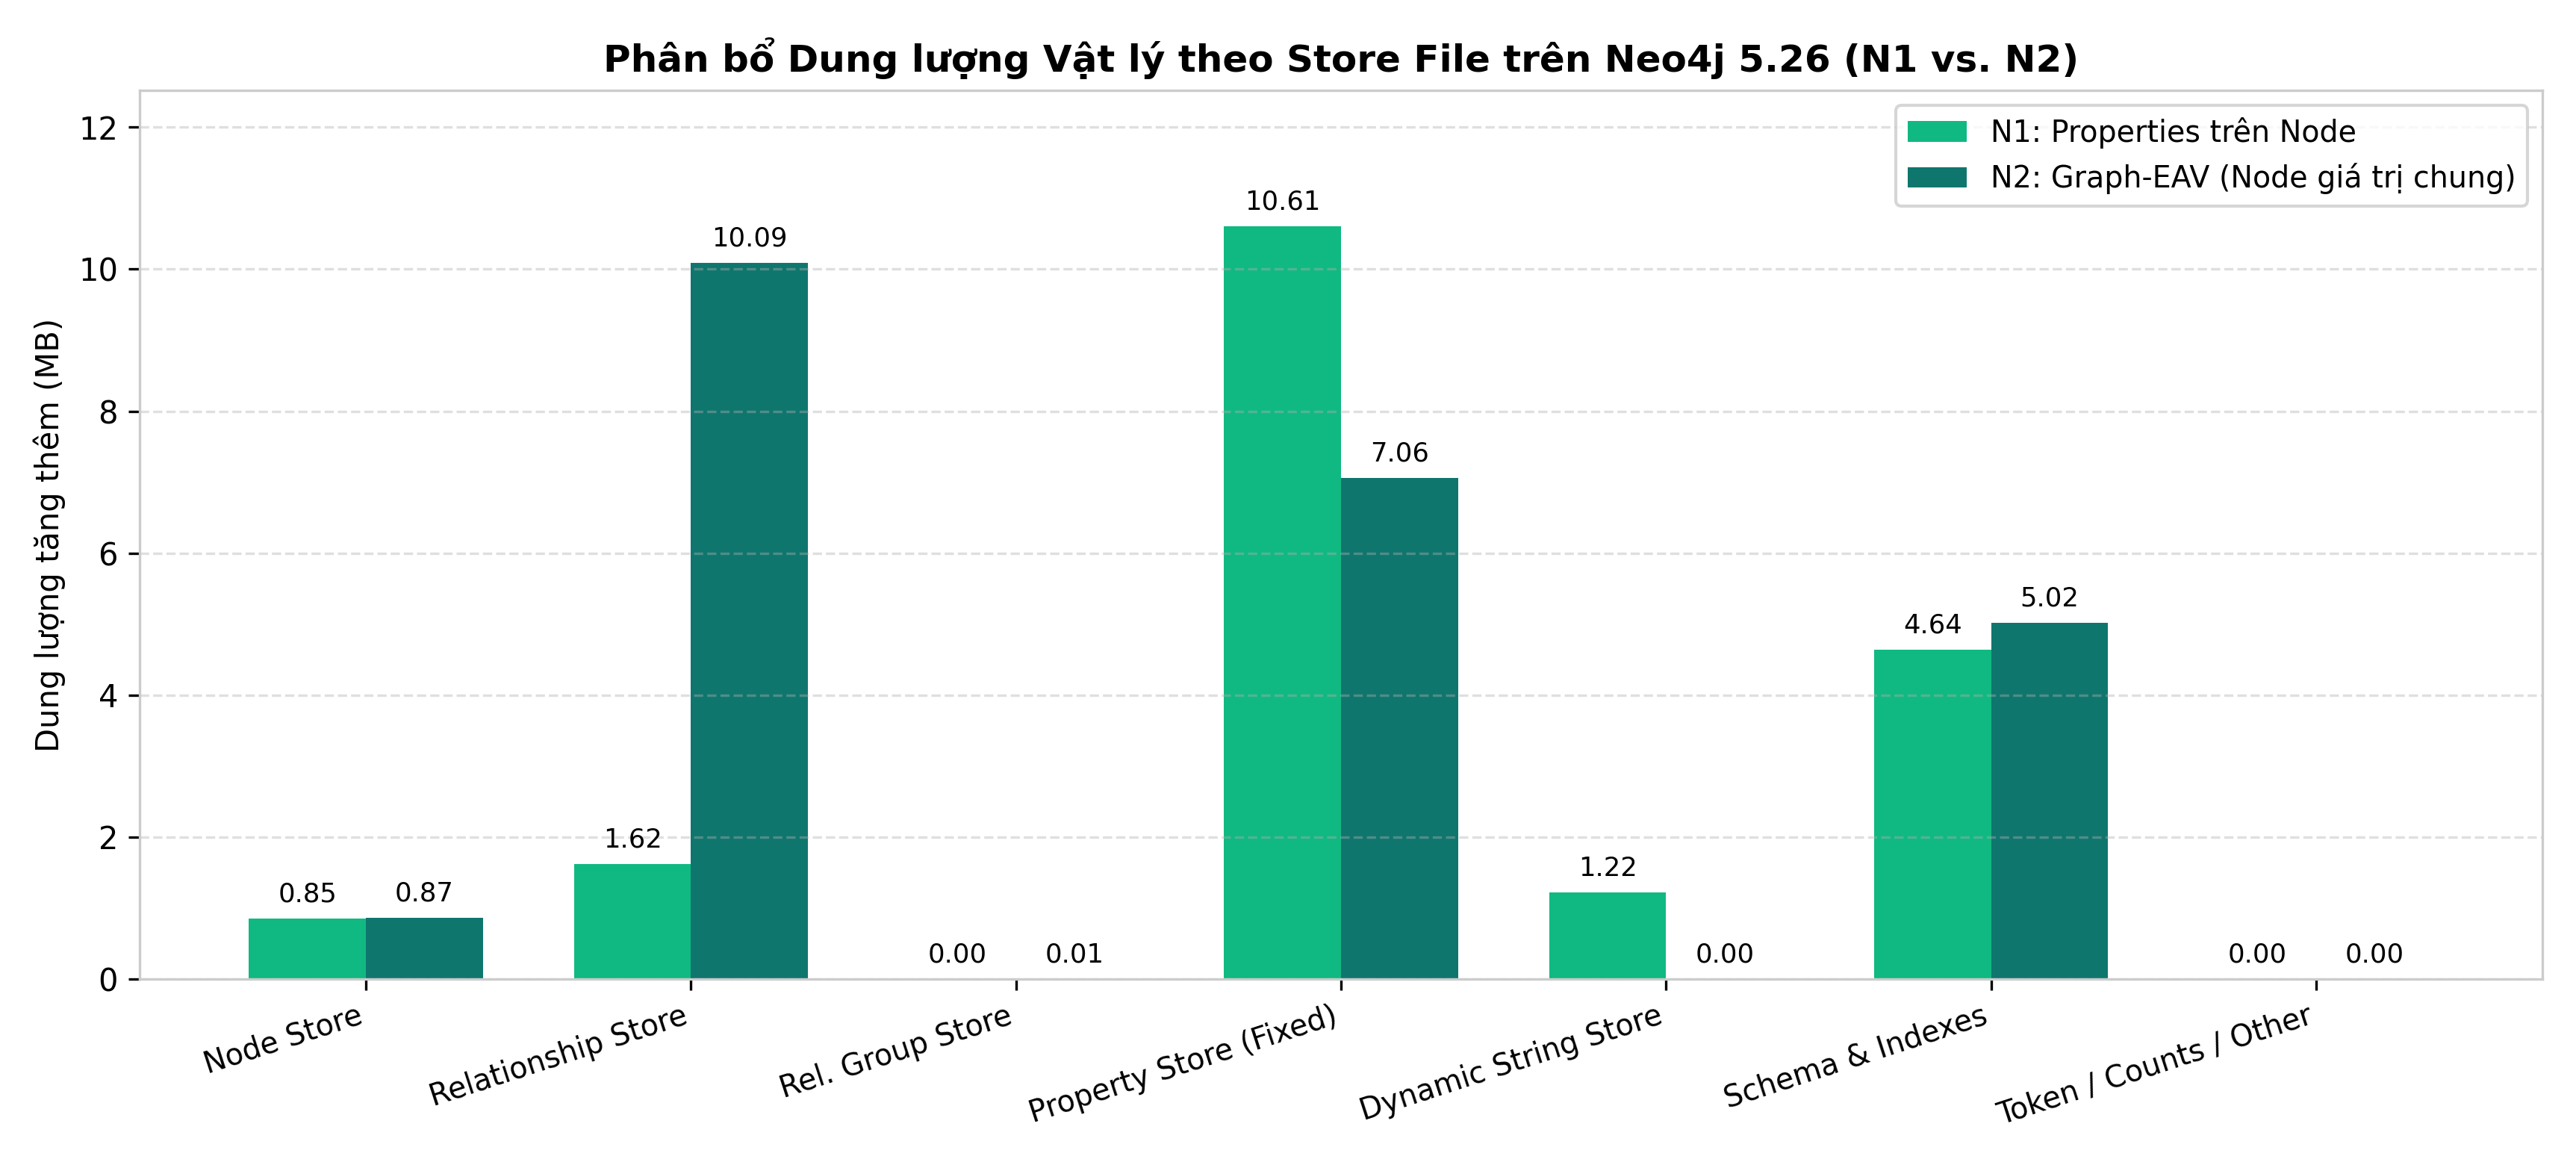
\includegraphics[width=0.95\textwidth]{report/images/topic1_neo4j_store_breakdown.png}
  \caption{Phân bổ dung lượng vật lý theo Store File trên Neo4j 5.26 (N1 vs. N2)}
  \label{fig:t1_neo4j_stores}
\end{figure}

Số liệu đo tại Bảng~\ref{tab:t1_neo4j_stores} và Hình~\ref{fig:t1_neo4j_stores} cho thấy rõ sự dịch chuyển dung lượng giữa các Store File: mô hình \texttt{N1} giữ thuộc tính trên nút làm \texttt{propertystore\_fixed} tăng \textbf{10,61 MB} và \texttt{propertystore\_strings} tăng \textbf{1,22 MB} (do lặp lại 10.000 chuỗi \texttt{isbn\_note}); ngược lại \texttt{N2} (Graph-EAV) triệt tiêu hoàn toàn phần tăng thêm của \texttt{propertystore\_strings} (\textbf{0,00 MB}) nhờ dùng chung nút giá trị, nhưng đẩy mạnh \texttt{relationshipstore} lên \textbf{10,09 MB} để lưu 260.000 cạnh \texttt{[:T1\_HAS\_ATTR]}. Đồng thời, thí nghiệm \textit{Space Reuse} trên 1.000 nút \texttt{:T1DeleteDemo} ghi nhận kích thước tổng trước khi chèn là \textbf{45.457.408 bytes} (\texttt{nodestore = 1.900.544 bytes}), sau khi chèn và checkpoint tăng lên \textbf{46.080.000 bytes} (\texttt{nodestore = 1.916.928 bytes}), và sau khi xóa bằng \texttt{DETACH DELETE} rồi checkpoint lại vẫn giữ mức \textbf{46.096.384 bytes} (\texttt{nodestore = 1.916.928 bytes}), xác nhận tệp vật lý không tự co lại ngay sau khi xóa dữ liệu.

\paragraph{Kịch bản 2: So sánh dung lượng lưu trữ vật lý trên 50.000 biến thể sản phẩm:}
Kịch bản 2 đối chiếu tổng không gian lưu trữ vật lý khi chứa cùng 50.000 biến thể đa ngành hàng giữa 6 mô hình SQL Server (đo từ \texttt{sys.partitions}, \texttt{sys.allocation\_units}, \texttt{sys.dm\_db\_index\_physical\_stats}) và 2 mô hình Neo4j:

\begin{lstlisting}[language=SQL, caption={Trích lược đồ EAV nén PAGE, Native JSON 2025 và SPARSE NULL}, label={lst:t1_sql_models}]
-- M1_EAV_PageComp: EAV value table + covering index with DATA_COMPRESSION = PAGE
CREATE TABLE dbo.T1_Variant_Attr_Values_PageComp (
    variant_id INT NOT NULL, attr_id INT NOT NULL, attr_value NVARCHAR(200) NOT NULL,
    CONSTRAINT PK_T1_EAV_PC PRIMARY KEY CLUSTERED (variant_id, attr_id)
        WITH (DATA_COMPRESSION = PAGE)
);
CREATE NONCLUSTERED INDEX IX_T1_EAV_PC_AttrVal
ON dbo.T1_Variant_Attr_Values_PageComp (attr_id, attr_value)
WITH (DATA_COMPRESSION = PAGE);

-- M2b_JsonNative: Hybrid Relational + Native `json` data type (SQL Server 2025)
CREATE TABLE dbo.T1_Variants_JsonNative (
    variant_id INT NOT NULL PRIMARY KEY CLUSTERED, product_id INT NOT NULL,
    category_name NVARCHAR(30) NOT NULL, sku NVARCHAR(40) NOT NULL,
    price DECIMAL(18,2) NOT NULL, stock_qty INT NOT NULL,
    attributes json NOT NULL
);

-- M3_Sparse: Wide Table with SPARSE NULL columns (0 bytes per NULL value)
CREATE TABLE dbo.T1_Variants_Sparse (
    variant_id INT NOT NULL PRIMARY KEY CLUSTERED, product_id INT NOT NULL,
    category_name NVARCHAR(30) NOT NULL, sku NVARCHAR(40) NOT NULL,
    price DECIMAL(18,2) NOT NULL, stock_qty INT NOT NULL,
    color NVARCHAR(20) NULL, storage_gb INT SPARSE NULL, ram_gb INT SPARSE NULL,
    cpu_model NVARCHAR(40) SPARSE NULL, apparel_size NVARCHAR(10) SPARSE NULL,
    isbn_note NVARCHAR(200) SPARSE NULL -- 20 sparse category columns in total
);
\end{lstlisting}

\begin{table}[htbp]
  \centering
  \scriptsize
  \setlength{\tabcolsep}{3.5pt}
  \renewcommand{\arraystretch}{1.25}
  \setlength{\emergencystretch}{2em}
  \caption{So sánh dung lượng lưu trữ vật lý trên 50.000 biến thể sản phẩm (8 mô hình)}
  \label{tab:t1_storage_50k}
  \begin{tabular}{|p{3.4cm}|p{2.35cm}|p{1.35cm}|p{1.4cm}|p{1.4cm}|p{1.0cm}|p{1.3cm}|}
    \hline
    \textbf{Mô hình lưu trữ} & \textbf{DBMS} & \textbf{Data (MB)} & \textbf{Index (MB)} & \textbf{Total (MB)} & \textbf{B/Var} & \textbf{In-Row Pages} \\
    \hline
    \texttt{M3\_Sparse} (SPARSE)       & SQL Server 2025 & 10,203 &  0,000 & \textbf{10,203} & 214,0 & 1.306 \\ \hline
    \texttt{M1\_EAV\_PageComp}         & SQL Server 2025 &  7,031 &  3,305 & \textbf{10,336} & 216,8 & 1.323 \\ \hline
    \texttt{Control\_WideNoSparse}     & SQL Server 2025 & 10,828 &  0,000 & \textbf{10,828} & 227,1 & 1.386 \\ \hline
    \texttt{M2b\_JsonNative}           & SQL Server 2025 & 14,133 &  0,000 & \textbf{14,133} & 296,4 & 1.809 \\ \hline
    \texttt{M2a\_JsonText}             & SQL Server 2025 & 16,648 &  0,000 & \textbf{16,648} & 349,1 & 2.131 \\ \hline
    \texttt{N1\_Neo4j\_Properties}     & Neo4j 5.26      & 14,305 &  4,641 & \textbf{18,945} & 397,3 & --    \\ \hline
    \texttt{N2\_Neo4j\_GraphEAV}       & Neo4j 5.26      & 18,031 &  5,023 & \textbf{23,055} & 483,5 & --    \\ \hline
    \texttt{M1\_EAV} (Không nén)       & SQL Server 2025 & 13,516 & 11,250 & \textbf{24,766} & 519,4 & 3.170 \\ \hline
  \end{tabular}
\end{table}

\begin{figure}[H]
  \centering
  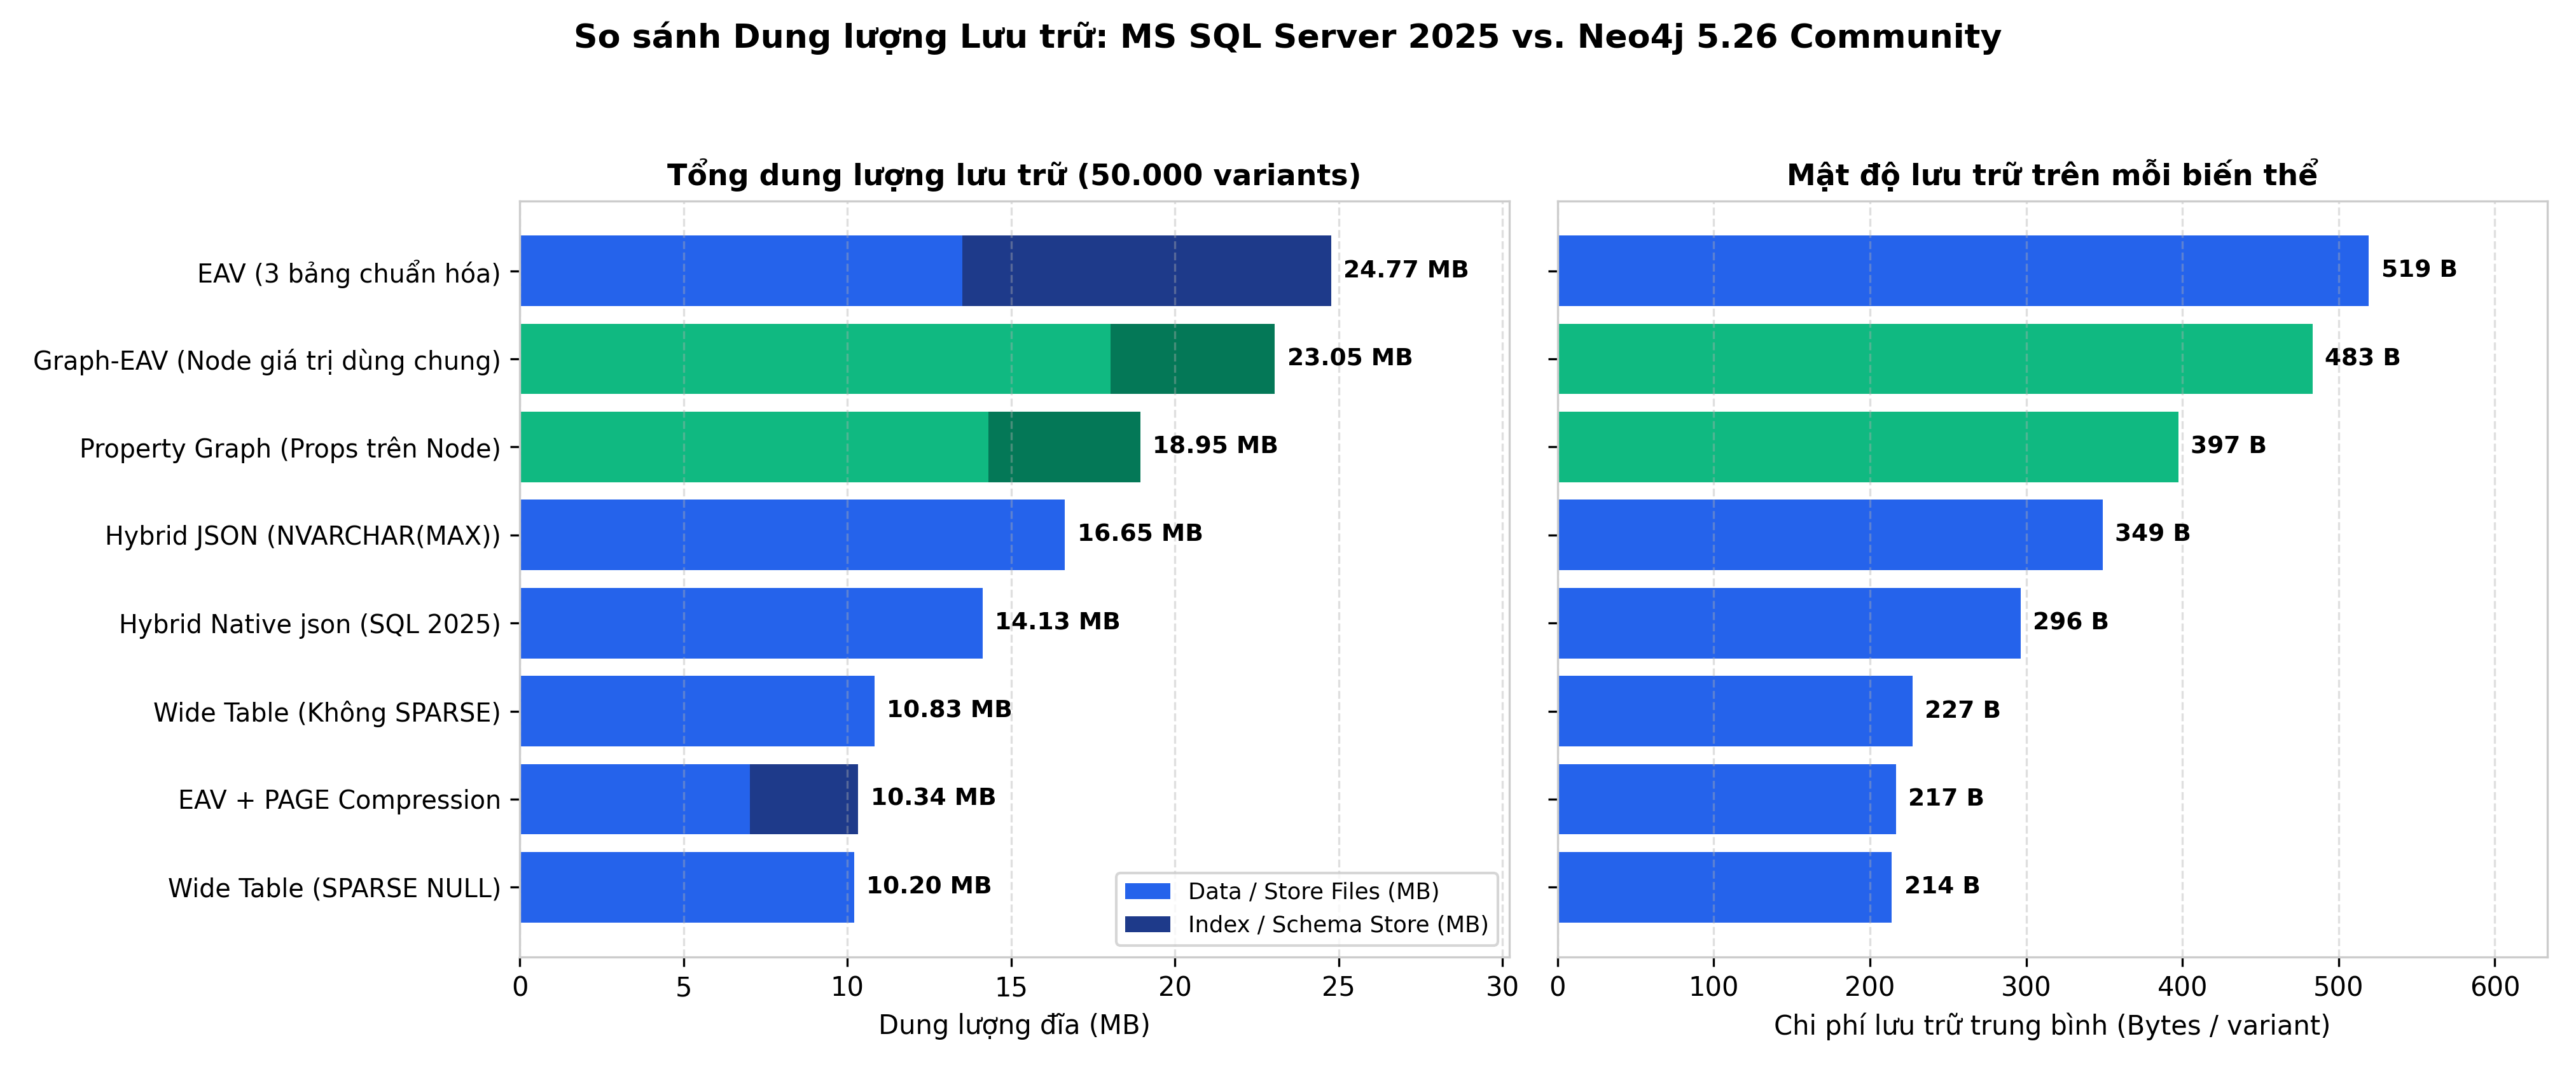
\includegraphics[width=\textwidth]{report/images/topic1_storage_comparison.png}
  \caption{So sánh tổng dung lượng đĩa và mật độ lưu trữ trên mỗi biến thể (50.000 variants)}
  \label{fig:t1_storage_comp}
\end{figure}

Kết quả tại Bảng~\ref{tab:t1_storage_50k} và Hình~\ref{fig:t1_storage_comp} (tất cả bảng SQL đều có 0 trang \texttt{ROW\_OVERFLOW\_DATA} và 0 trang \texttt{LOB\_DATA}) cho thấy bốn điểm nổi bật:
\begin{enumerate}
  \item \textbf{Tác động của nén \texttt{PAGE} lên EAV:} Khi không nén, \texttt{M1\_EAV} tốn nhiều dung lượng nhất (\textbf{24,77 MB}, 519,4 B/biến thể) do nhân thành 260.000 dòng dọc kèm chỉ mục phụ chiếm 11,25 MB. Khi bật \texttt{DATA\_COMPRESSION = PAGE}, nén từ điển và tiền tố nội trang kéo tổng dung lượng giảm \textbf{58,3\%} xuống còn \textbf{10,34 MB} (từ 3.170 xuống 1.323 trang 8 KB).
  \item \textbf{Ưu thế của kiểu \texttt{json} gốc trên SQL Server 2025:} Nhờ lưu nhị phân đã phân tích cú pháp sẵn, \texttt{M2b\_JsonNative} chỉ tiêu tốn \textbf{14,13 MB} (286,37 B/dòng), tiết kiệm trực tiếp \textbf{15,1\%} dung lượng so với \texttt{M2a\_JsonText} lưu văn bản UTF-16 (\textbf{16,65 MB}, 333,79 B/dòng).
  \item \textbf{Hiệu quả thực tế của \texttt{SPARSE NULL}:} Với tỷ lệ \texttt{NULL} 80\% trên 20 cột đặc thù, mô hình \texttt{M3\_Sparse} đạt dung lượng nhỏ nhất (\textbf{10,20 MB}), tiết kiệm \textbf{5,8\%} so với bảng đối chứng \texttt{Control\_WideNoSparse} (\textbf{10,83 MB}) do phần lớn cột chuỗi biến thiên \texttt{NVARCHAR} vốn đã nhỏ gọn khi \texttt{NULL} trong khi cột Sparse phải bù thêm chi phí \textit{Sparse Vector} cho các giá trị khác \texttt{NULL}.
  \item \textbf{Chi phí cấu trúc của Neo4j:} Cả \texttt{N1} (\textbf{18,95 MB}) và \texttt{N2} (\textbf{23,05 MB}) đều lớn hơn các mô hình lai JSON và Sparse của SQL Server vì phải lưu thêm các tệp con trỏ quan hệ hai chiều và chỉ mục nhãn (\texttt{schema\_indexes} chiếm 4,64--5,02 MB).
\end{enumerate}

\paragraph{Kịch bản 3: So sánh khả năng mở rộng Schema (Schema Evolution) và hiệu năng truy vấn (d), (a), (c):}
Kịch bản 3 kiểm tra tốc độ thích ứng khi nghiệp vụ thay đổi và hiệu năng trên nhóm truy vấn thuộc phạm vi Thành viên 1: (1) bổ sung thuộc tính mới \texttt{battery\_mAh = 5000} cho toàn bộ \textbf{10.000 biến thể Smartphones}; (2) chạy \textbf{Truy vấn (d)} điều kiện đơn lọc \texttt{color = 'Black'} (khớp chính xác \textbf{8.000 biến thể} ở cả 8 mô hình, đo trung bình 3 lần sau warmup kèm \texttt{logical reads} / \texttt{PROFILE db hits}); và (3) chạy \textbf{Truy vấn (a)} chèn thuộc tính lạ \texttt{waterproof\_ip = 'IP68'} cùng \textbf{Truy vấn (c)} cập nhật giá và màu cho \texttt{variant\_id = 1}:

\begin{lstlisting}[language=SQL, caption={Thực nghiệm Schema Evolution và truy vấn (d)/(a)/(c) trên MS SQL Server 2025}, label={lst:t1_sql_evo}]
-- 1. Schema Evolution: Wide/Sparse require DDL ALTER TABLE (Sch-M lock)
ALTER TABLE dbo.T1_Variants_Sparse ADD battery_mAh INT SPARSE NULL;
UPDATE dbo.T1_Variants_Sparse
SET battery_mAh = 5000 WHERE category_name = N'Smartphones';

--    Hybrid Native json adds attribute via DML .modify() with ZERO DDL
UPDATE dbo.T1_Variants_JsonNative
SET attributes.modify('$.battery_mAh', 5000)
WHERE category_name = N'Smartphones';

-- 2. Query (d) Single Condition: filter color = 'Black' (8,000 matches)
SELECT COUNT(*) FROM dbo.T1_Variant_Attr_Values_PageComp v
JOIN dbo.T1_Attributes a ON a.attr_id = v.attr_id
WHERE a.attr_name = N'color' AND v.attr_value = N'Black';

SELECT COUNT(*) FROM dbo.T1_Variants_JsonNative
WHERE JSON_VALUE(attributes, '$.color') = N'Black';

-- 3. Query (a) Insert novel attribute & Query (c) Point Update (FR-07)
INSERT INTO dbo.T1_Variants_JsonNative
VALUES (999999, 1, N'Smartphones', N'SKU-DEMO-IP68', 1199.00, 15,
        '{"color":"Black","waterproof_ip":"IP68"}');
UPDATE dbo.T1_Variants_JsonNative
SET price = price + 10.00, attributes.modify('$.color', N'Matte Black')
WHERE variant_id = 1;
\end{lstlisting}

\begin{lstlisting}[language={}, caption={Thực nghiệm Schema Evolution và truy vấn (d)/(a)/(c) trên Neo4j 5}, label={lst:t1_neo_evo}, morekeywords={MATCH,SET,RETURN,count,MERGE,WITH,PROFILE,WHERE,CREATE}, sensitive=false, morecomment={[l]{//}}, morestring={[b]'}]
// 1. Schema Evolution: N1 (SET property, 0 DDL) & N2 (Shared node + 10k edges)
MATCH (v:T1VariantProp {category: 'Smartphones'})
SET v.battery_mAh = 5000 RETURN count(v);

MERGE (a:T1AttrValue {name: 'battery_mAh', value: '5000'})
WITH a MATCH (v:T1VariantGraph {category: 'Smartphones'})
MERGE (v)-[:T1_HAS_ATTR]->(a) RETURN count(v);

// 2. Query (d) Single Condition: LabelScan (N1) vs Index-Free Adjacency (N2)
PROFILE MATCH (v:T1VariantProp) WHERE v.color = 'Black' RETURN count(v);
PROFILE MATCH (:T1AttrValue {name: 'color', value: 'Black'})
              <-[:T1_HAS_ATTR]-(v:T1VariantGraph)
RETURN count(v);

// 3. Query (a) Insert novel property & Query (c) Point Update
MATCH (p:T1Product {product_id: 1})
CREATE (p)-[:T1_HAS_VARIANT]->(:T1VariantProp {
  variant_id: 999999, sku: 'SKU-DEMO-IP68', price: 1199.0,
  color: 'Black', waterproof_ip: 'IP68'
});
MATCH (v:T1VariantProp {variant_id: 1})
SET v.price = v.price + 10.0, v.color = 'Matte Black';
\end{lstlisting}

\begin{table}[htbp]
  \centering
  \scriptsize
  \setlength{\tabcolsep}{3.5pt}
  \renewcommand{\arraystretch}{1.25}
  \setlength{\emergencystretch}{2em}
  \caption{Kết quả thực nghiệm Schema Evolution (10.000 Smartphones) và Truy vấn (d) (8.000 kết quả)}
  \label{tab:t1_evo_query}
  \begin{tabular}{|p{3.3cm}|p{1.2cm}|p{1.1cm}|p{1.9cm}|p{2.4cm}|p{2.1cm}|}
    \hline
    \textbf{Mô hình} & \textbf{Evo (ms)} & \textbf{Qd (ms)} & \textbf{Chi phí đọc} & \textbf{Linh hoạt Schema} & \textbf{An toàn kiểu} \\
    \hline
    \texttt{M1\_EAV}               &   645,12 &          2,03 &     32 \textit{reads} & Cao (Không DDL)         & Yếu (\texttt{NVARCHAR}) \\ \hline
    \texttt{M1\_EAV\_PageComp}     &   737,39 & \textbf{1,06} & \textbf{13 \textit{reads}} & Cao (Không DDL)    & Yếu (\texttt{NVARCHAR}) \\ \hline
    \texttt{M2a\_JsonText}         &   563,72 &        267,00 &  2.887 \textit{reads} & Cao (\texttt{JSON\_\allowbreak MODIFY}) & TB (\texttt{ISJSON}) \\ \hline
    \texttt{M2b\_JsonNative}       &   426,33 &        267,87 &  3.611 \textit{reads} & Cao (\texttt{.modify()}) & TB (Native JSON) \\ \hline
    \texttt{M3\_Sparse}            &   366,21 &         14,84 &  1.904 \textit{reads} & Thấp (DDL \texttt{Sch-M}) & Mạnh (Định kiểu) \\ \hline
    \texttt{Control\_WideNoSparse} &   304,63 &         13,61 &  1.474 \textit{reads} & Thấp (DDL \texttt{Sch-M}) & Mạnh (Định kiểu) \\ \hline
    \texttt{N1\_Neo4j\_Properties} &   758,00 &        123,33 & 100.001 \textit{hits} & Rất cao (0 DDL)         & Yếu (Community) \\ \hline
    \texttt{N2\_Neo4j\_GraphEAV}   & 1.854,00 &         80,33 & 16.004 \textit{hits}  & Rất cao (0 DDL)         & TB (\texttt{AttrValue}) \\ \hline
  \end{tabular}
\end{table}

\begin{figure}[H]
  \centering
  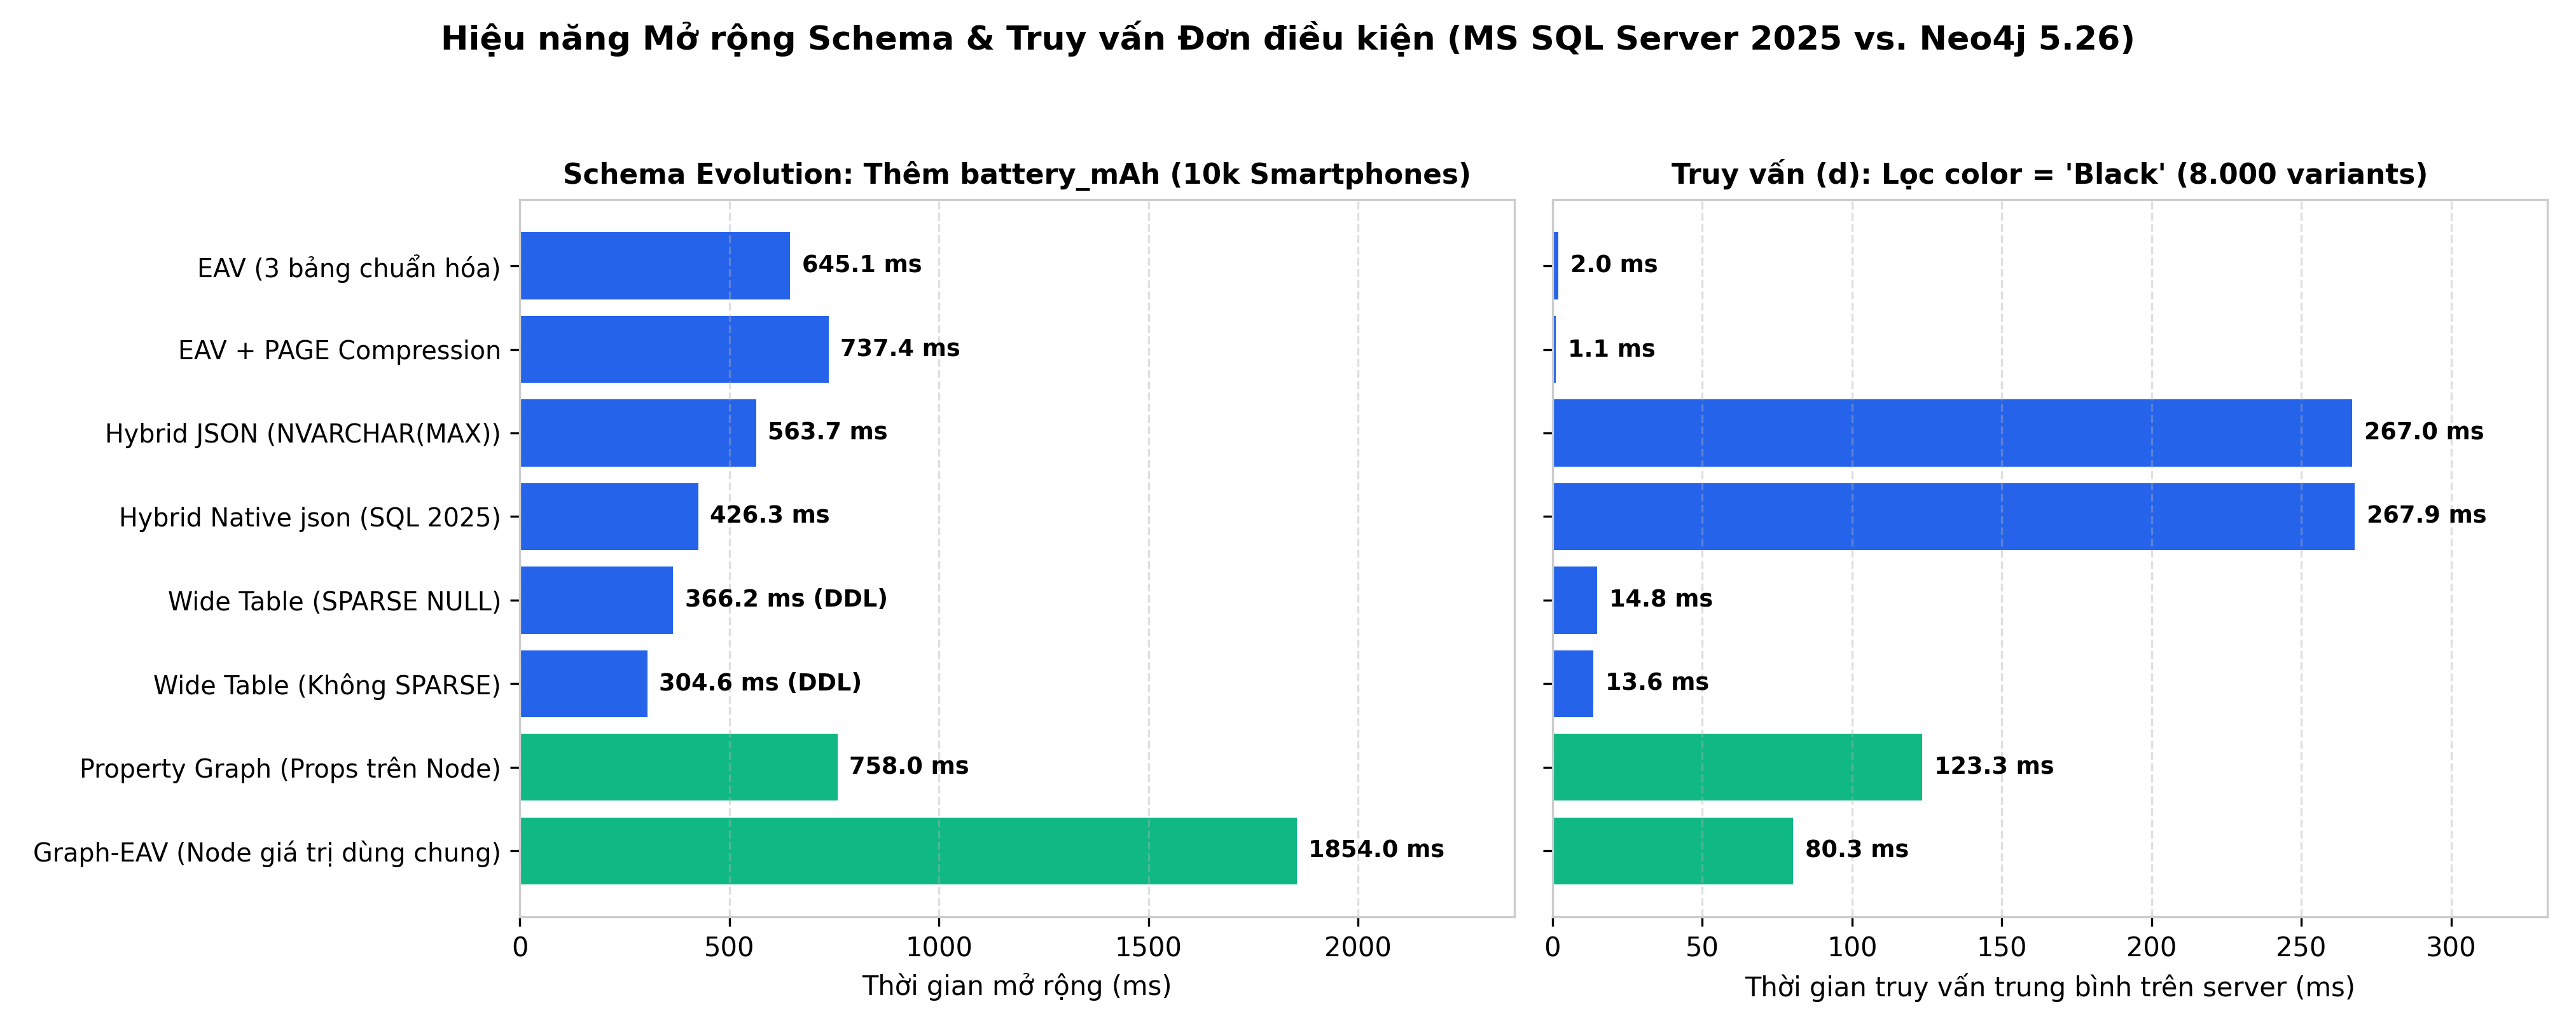
\includegraphics[width=\textwidth]{report/images/topic1_evolution_query.png}
  \caption{Hiệu năng mở rộng Schema và truy vấn đơn điều kiện (MS SQL Server 2025 vs. Neo4j 5.26)}
  \label{fig:t1_evo_query}
\end{figure}

Từ kết quả ở Bảng~\ref{tab:t1_evo_query} và Hình~\ref{fig:t1_evo_query}, có thể phân tích rõ các đánh đổi sau:
\begin{itemize}
  \item \textbf{Mở rộng Schema (\texttt{battery\_mAh}):} Hai bảng rộng \texttt{M3\_Sparse} (366,21 ms) và \texttt{Control\_WideNoSparse} (304,63 ms) phải dùng \texttt{ALTER TABLE} chiếm khóa \textbf{\texttt{Sch-M} (Schema Modification Lock)}, có nguy cơ chặn các giao dịch đồng thời trên hệ thống lớn. Ngược lại, \texttt{M2b\_JsonNative} hoàn tất mở rộng bằng DML \texttt{.modify()} trong \textbf{426,33 ms} (nhanh hơn 24,4\% so với \texttt{JSON\_MODIFY} của \texttt{M2a} ở mức 563,72 ms) mà không cần DDL. Trên Neo4j, \texttt{N1} mở rộng rất gọn bằng \texttt{SET} (758,00 ms), còn \texttt{N2} tốn 1.854,00 ms vì phải tạo mới 10.000 cạnh quan hệ trong \texttt{Relationship Store}.
  \item \textbf{Truy vấn (d) (\texttt{color = 'Black'}):} \texttt{M1\_EAV\_PageComp} đạt tốc độ nhanh nhất (\textbf{1,06 ms}, chỉ \textbf{13 logical reads}) nhờ chỉ mục bao phủ nén \texttt{PAGE}. Hai mô hình JSON chưa tạo chỉ mục computed column phải quét toàn bảng và phân tích JSON nên mất 267,00--267,87 ms. Trên Neo4j, \texttt{N2\_Neo4j\_GraphEAV} (\textbf{80,33 ms}, \textbf{16.004 db hits}) giảm được \textbf{84\% số lần truy cập CSDL} so với \texttt{N1} (\textbf{123,33 ms}, \textbf{100.001 db hits}) do \texttt{N1} phải quét toàn bộ 50.000 nút (\texttt{NodeByLabelScan}), còn \texttt{N2} định vị trực tiếp nút \texttt{:T1AttrValue} và đi theo 8.000 cạnh liền kề bằng \textit{Index-Free Adjacency}.
  \item \textbf{Truy vấn (a) Insert \& (c) Update (FR-07):} Khi thử chèn biến thể mới có thuộc tính lạ \texttt{waterproof\_ip = 'IP68'}, mô hình \texttt{M3\_Sparse} lập tức bị từ chối với lỗi \textbf{Msg 207} (\textit{Invalid column name 'waterproof\_ip'}), thể hiện tính khắt khe của \textit{Schema-on-Write}; trong khi \texttt{M2b\_JsonNative} chèn thành công trong \textbf{5,88 ms} và cập nhật giá + màu cục bộ bằng \texttt{.modify()} chỉ mất \textbf{3,00 ms}. Trên Neo4j, lệnh Cypher đơn lẻ tạo thuộc tính mới kèm dọn dẹp ghi nhận \textbf{669,00 ms} và lệnh cập nhật + khôi phục ghi nhận \textbf{307,00 ms} (do là lượt chạy đơn chưa làm nóng bộ đệm kế hoạch thực thi và bao gồm thao tác dọn dẹp trong cùng phiên \texttt{cypher-shell}).
\end{itemize}

\subsubsection{Đánh giá và quyết định}

Bảng~\ref{tab:t1_summary} tổng hợp các đặc tính cốt lõi về lưu trữ và quản trị dữ liệu giữa MS SQL Server 2025 và Neo4j 5.26:

\begin{table}[htbp]
  \centering
  \footnotesize
  \setlength{\tabcolsep}{4pt}
  \renewcommand{\arraystretch}{1.25}
  \setlength{\emergencystretch}{2em}
  \caption{So sánh tổng hợp cơ chế Data Storage \& Management giữa MS SQL Server và Neo4j}
  \label{tab:t1_summary}
  \begin{tabular}{|p{2.9cm}|p{5.0cm}|p{5.0cm}|}
    \hline
    \textbf{Tiêu chí} & \textbf{MS SQL Server (2025)} & \textbf{Neo4j (5.26 LTS)} \\
    \hline
    Mô hình dữ liệu & Relational Model & Labeled Property Graph \\ \hline
    Thiết kế Schema & Schema-on-Write (ép ràng buộc khi ghi) & Schema-Optional (linh hoạt thuộc tính) \\ \hline
    Tổ chức dữ liệu & Tables, Rows, Columns & Nodes, Relationships, Properties \\ \hline
    Đơn vị lưu trữ & Page 8 KB, Extent 64 KB & Record Store (Aligned) hoặc Block Store \\ \hline
    Cấu trúc lưu trữ & Heap, Clustered Index B+Tree & Node, Relationship, Property Store \\ \hline
    Truy xuất quan hệ & Foreign Key và JOIN & Index-Free Adjacency ($O(1)$/bước nhảy) \\ \hline
    Dữ liệu lớn / động & Row Overflow, LOB, Native \texttt{json}, Sparse & Inline Storage và Dynamic Storage \\ \hline
    Bộ nhớ đệm & Buffer Pool & Off-Heap Page Cache (tách JVM Heap) \\ \hline
    Cơ chế nén & Row Compression, Page Compression & Phụ thuộc Store Format \\ \hline
    Mở rộng thuộc tính & \texttt{ALTER TABLE} (\texttt{Sch-M}) hoặc EAV/JSON & \texttt{SET}/\texttt{CREATE} tức thì (0 DDL) \\ \hline
    Phục hồi dữ liệu & Transaction Log, Checkpoint, REDO/UNDO & Transaction Log, Checkpoint, Recovery \\ \hline
    Thu hồi không gian & Ghost Cleanup, REBUILD, REORGANIZE & Space Reuse và Defragmentation \\ \hline
  \end{tabular}
\end{table}

\paragraph{Quyết định lựa chọn cho hệ thống E-Commerce:} Từ phân tích lý thuyết và số liệu thực nghiệm trên, nhóm quyết định chọn \textbf{MS SQL Server} làm hệ quản trị cơ sở dữ liệu chính cho nền tảng thương mại điện tử đa gian hàng vì ba lý do then chốt:

\begin{enumerate}
  \item \textbf{Bảo toàn tính toàn vẹn bằng Schema-on-Write:} Hệ thống E-Commerce xoay quanh các thực thể giao dịch tài chính và tồn kho (\texttt{Users}, \texttt{Sellers}, \texttt{Products}, \texttt{Orders}, \texttt{Order\_Details}, \texttt{Vouchers}), đòi hỏi cơ chế kiểm tra kiểu dữ liệu, khóa ngoại và ràng buộc \texttt{CHECK} nghiêm ngặt ngay tại tầng Storage Engine (như đã chứng minh bằng lỗi 547 khi chặn giá âm).
  \item \textbf{Hiệu quả nén và lưu trữ đa dạng trên trang 8 KB:} Kiến trúc Page 8 KB kết hợp \texttt{DATA\_COMPRESSION = PAGE} (216,8 B/biến thể) và mô hình lai Native \texttt{json} (296,4 B/biến thể, 0 DDL khi mở rộng) giúp tối ưu dung lượng đĩa vượt trội so với Neo4j (397,3--483,5 B/biến thể), vừa giữ trọn lợi thế quan hệ vừa linh hoạt cho biến thể sản phẩm.
  \item \textbf{Khả năng kết hợp Polyglot Persistence trong tương lai:} Neo4j không phù hợp thay thế cho CSDL giao dịch chính do thiếu chuẩn hóa ràng buộc bảng, nhưng rất lý tưởng để vận hành song song cho các phân hệ phân tích đồ thị nhiều tầng như hệ thống gợi ý sản phẩm cá nhân hóa hoặc phát hiện gian lận liên kết giữa \texttt{Users} -- \texttt{Orders} -- \texttt{Sellers}.
\end{enumerate}


% ==============================================================================
% CÁC ĐOẠN CẦN BỔ SUNG VÀO CÁC VỊ TRÍ KHÁC TRONG main.tex (BỎ COMMENT KHI DÁN)
% ==============================================================================
%
% --- [1] Dòng bổ sung vào Bảng 1 (Danh sách thành viên & Phân công công việc) ---
% 2 & Trần Quốc Hiền & 2310992 &
%   - Nghiên cứu chủ đề Data Storage \& Schema Design (MS SQL Server vs Neo4j) \newline
%   - Thiết kế lược đồ ECommerceDB và hiện thực FR-02, FR-07, AuthModule & 100\% \\ \hline
%
% --- [2] Sửa lỗi tiêu đề "Tài liệu" bị cắt chữ ở cuối main.tex (nếu dùng babel vietnamese) ---
% Thêm dòng này trước \begin{document} trong main.tex:
% \addto\captionsvietnamese{\renewcommand{\refname}{Tài liệu tham khảo}}
%
% --- [3] 9 Tài liệu tham khảo nối tiếp sau [10] trong \begin{thebibliography} ---
% \bibitem{t1_date2004}
% C.~J. Date, \textit{An Introduction to Database Systems}, 8th~ed. Pearson, 2004.
%
% \bibitem{t1_silberschatz2019}
% A.~Silberschatz, H.~F. Korth, and S.~Sudarshan, \textit{Database System Concepts}, 7th~ed. McGraw-Hill, 2019.
%
% \bibitem{t1_delaney2012}
% K.~Delaney et~al., \textit{Microsoft SQL Server 2012 Internals}. Microsoft Press, 2012.
%
% \bibitem{t1_mspages}
% Microsoft Learn, \textit{Pages and Extents Architecture Guide -- SQL Server}. [Online]. Available: \url{https://learn.microsoft.com/en-us/sql/relational-databases/pages-and-extents-architecture-guide}
%
% \bibitem{t1_mssparse}
% Microsoft Learn, \textit{Use Sparse Columns -- SQL Server}. [Online]. Available: \url{https://learn.microsoft.com/en-us/sql/relational-databases/tables/use-sparse-columns}
%
% \bibitem{t1_mscomp}
% Microsoft Learn, \textit{Data Compression -- SQL Server}. [Online]. Available: \url{https://learn.microsoft.com/en-us/sql/relational-databases/data-compression/data-compression}
%
% \bibitem{t1_msnativejson}
% Microsoft Learn, \textit{JSON data type (SQL Server 2025)}. [Online]. Available: \url{https://learn.microsoft.com/en-us/sql/t-sql/data-types/json-data-type}
%
% \bibitem{t1_robinson2015}
% I.~Robinson, J.~Webber, and E.~Eifrem, \textit{Graph Databases: New Opportunities for Connected Data}, 2nd~ed. O'Reilly Media, 2015.
%
% \bibitem{t1_neo4jops}
% Neo4j Documentation, \textit{Operations Manual: Store Formats, Memory Configuration, Transaction Logs and Checkpointing}. [Online]. Available: \url{https://neo4j.com/docs/operations-manual/current/}
